\documentclass[a5paper, 10pt, openany]{book} % A5 paper size

% \usepackage[paperwidth=148mm, paperheight=210mm, top=1.27cm, bottom=1.27cm, inner=1.9cm, outer=1.27cm, headsep=1.5cm, footskip=1.75cm]{geometry} % Custom dimensions and margins
% Adjusted margins to ensure space for page numbers
\usepackage[paperwidth=148mm, paperheight=210mm, 
         top=1.27cm, bottom=2.5cm, inner=2.2cm, outer=1.27cm, 
         headsep=1.5cm, footskip=1.5cm]{geometry}


\usepackage[utf8]{inputenc}
\usepackage{ctex}

\usepackage{fancyhdr}
\pagestyle{fancy}
\fancyhf{} % Clear all header and footer fields
% \fancyfoot[C]{\thepage} % Center the page number at the bottom
% Define left and right page numbering
\fancyfoot[LE]{\thepage} % Left side for even pages
\fancyfoot[RO]{\thepage} % Right side for odd pages
% Ensure the chapter pages (plain style) also have this layout
\makeatletter
\let\ps@plain\ps@fancy
\makeatother


% *-----------------------------------------------------------------------*
% | Fonts and typography                                                  |
% *-----------------------------------------------------------------------*

% Set CJK main font (for Chinese/Japanese/Korean characters)

% \setmainfont{Times New Roman}
\setCJKmainfont{BabelStone Han}
% doesn't work
% \setCJKmainfont{JyutcitziWithSourceHanSerifTCRegular}[
% Renderer=Basic,
% UprightFont = * ,
% FallbackFonts={BabelStone Han}
% ]



% You can also use \newfontfamily for custom non-CJK fonts if needed
% \setCJKmainfont{JyutcitziWithPMingLiURegular}[Path = ./, Extension = .ttf]
% \setCJKmainfont{JyutcitziWithSourceHanSerifTCRegular}[Path = ./, Extension = .ttf]



\newfontfamily{\jczPMingLiU}{JyutcitziWithPMingLiURegular}[Path = ../fonts/, Extension = .ttf]
% This has the best rendition for latin characters 
\newfontfamily{\jcz}{JyutcitziWithSourceHanSerifTCRegular}[Path = ../fonts/, Extension = .ttf]
\newfontfamily{\batang}{batang}[Path = ../fonts/, Extension = .ttf]
\newCJKfontfamily\koreanfont{Batang}[Path = ../fonts/, Extension = .ttf]




% *-----------------------------------------------------------------------*
% | Formatting     |
% *-----------------------------------------------------------------------*
% Set global paragraph indentation and spacing
\setlength{\parindent}{2em} % Adjust this value for the desired indentation
\setlength{\parskip}{0pt}   % No space between paragraphs

% for quotes
\usepackage{epigraph} 


\makeatletter
\renewcommand{\@makefntext}[1]{\jcz{\@thefnmark.} #1}
\makeatother
% to control itemise spacing
\usepackage{enumitem}



% *-----------------------------------------------------------------------*
% | Math & Equations     |
% *-----------------------------------------------------------------------*
\usepackage{amsmath} % For advanced math formatting
\usepackage{amssymb} % For mathematical symbols
% \usepackage{tikz} % For drawing logic decision trees


% *-----------------------------------------------------------------------*
% | Table Management                                                      |
% *-----------------------------------------------------------------------*


\usepackage{graphicx}
\usepackage{array}
\usepackage{tabularx}
\usepackage{tabularray}
\usepackage{longtable}

\usepackage{float}      % Add the float package


\usepackage[table,xcdraw]{xcolor}
% 

% Load ruby package for furigana (Ruby text)
\usepackage{ruby}
% \renewcommand{\ruby}[2]{%
%   \ruby{\jcz{#1}}{\jcz{#2}}%
% }


% *-----------------------------------------------------------------------*
% | Chinese and Soochow Numerals               |
% *-----------------------------------------------------------------------*

% Define Chinese numerals for numbers 1-99
% 〇〡〢 〣 〤 〥 〦 〧 〨 〩 十 〹 〺 卅
% Include the numerals file
\input{styles/numerals.tex}

% *-----------------------------------------------------------------------*
% | Table of contents & Chapter for chapter management |
% *-----------------------------------------------------------------------*

\renewcommand{\figurename}{圗} % So figures would be labeled with 圗 instead of "figure"

% * * * Now for the table of contents
\renewcommand{\contentsname}{目錄} % Traditional Chinese characters for "Contents"
\setcounter{secnumdepth}{0} % no numbering for sections 
% Increase chapter title size in TOC
\usepackage{tocloft} % For customizing table of contents
\renewcommand{\cftchapfont}{\Large\bfseries} % Large and bold chapter titles
\renewcommand{\cftchappagefont}{\Large\bfseries} % Large and bold page numbers
\renewcommand{\cftchapnumwidth}{3em} % Adjust the width for chapter numbers (increase the space)

% Custom chapter numbering in the TOC with Soochow numerals
\renewcommand{\cftchapleader}{\cftdotfill{\cftsecdotsep}} % Dotted line between chapter and page number
\renewcommand{\cftchapaftersnum}{\quad} % Space between Soochow numeral and chapter title

% Redefine how chapter numbers are displayed in the TOC using Soochow numerals
\makeatletter
\renewcommand{\cftchapleader}{\cftdotfill{\cftsecdotsep}} % Dotted line between chapter and page number
\renewcommand{\cftchapaftersnum}{\quad} % Space between Soochow numeral and chapter title
% comment this out if you don't want to use the soochow numerlas
\renewcommand{\numberline}[1]{\soochowNumeral{#1}\hspace{1em}} % Use Soochow numerals for TOC chapter numbers
\makeatother


% create index - run \makeindex in the document
\usepackage{makeidx}
\makeindex



% % Custom chapter title formatting with Chinese numeral chapter numbers
\usepackage{titlesec}

% Custom chapter title formatting with Chinese numeral chapter numbers
\titleformat{\chapter}[block] % 'block' means the title appears on a new line
  {\Large\bfseries} % Font size and bold formatting for the title
  {\soochowNumeral{\thechapter}} % Chinese character for chapter number
  {1em} % Space between the number and the title
  {\Large} % Custom style for the chapter title itself (can modify)

% Remove the default LaTeX behavior of forcing new chapters to start on a new page
\makeatletter
\renewcommand\chapter{\if@openright\cleardoublepage\else\clearpage\fi
  \thispagestyle{plain}%
  \global\@topnum\z@
  \@afterindentfalse
  \secdef\@chapter\@schapter}
\makeatother




\usepackage{listings}
\usepackage{xcolor} % Optional, for colors in code
\lstset{
    language=Python,
    basicstyle=\ttfamily\small,
    keywordstyle=\color{blue},
    commentstyle=\color{green},
    stringstyle=\color{red},
    breaklines=true,
    numbers=left,
    numberstyle=\tiny,
    stepnumber=1,
    frame=single,
    captionpos=b
}

\usepackage[all]{genealogytree}

% for vertical Chinese boxes
\usepackage{graphicx} % for \rotatebox

\newfontlanguage{Chinese}{CHN}

\setCJKfamilyfont{BabelStoneVert}[RawFeature={vertical;+vert},Script=CJK,Language=Chinese,Vertical=RotatedGlyphs]{BabelStone Han}

\newcommand*\CJKmovesymbol[1]{\raise.35em\hbox{#1}}
\newcommand*\CJKmove{\punctstyle{plain}% do not modify the spacing between punctuations
  \let\CJKsymbol\CJKmovesymbol
  \let\CJKpunctsymbol\CJKsymbol}

% Define a new environment for vertical text
\newcommand{\VertCell}[1]{\rotatebox{-90}{\CJKfamily{BabelStoneVert}\CJKmove #1}}


% IDC - ideographic description characters
% https://en.wikipedia.org/wiki/Chinese_character_description_languages#Ideographic_Description_Sequences

\newcommand{\superimpose}[2]{{%
  \ooalign{%
    \hfil$\m@th\text{#1}\@firstoftwo\text{#2}$\hfil\cr
    \hfil$\m@th\text{#1}\@secondoftwo\text{#2}$\hfil\cr
  }%
}}


% Define the \tb command

\newcommand{\tb}[2]{%
\scalebox{2}[1]{
\ooalign{%
    \hfil\raisebox{0.25em}{\text{\scalebox{0.33}{#1}}}\hfil\cr % Top text, squished and raised
    \hfil\raisebox{-0.25em}{\text{\scalebox{0.33}{#2}}}\hfil\cr % Bottom text, squished and lowered
  }%
  }
}

% The \lr command - can be combined with \tb
\newcommand{\lr}[2]{
  \scalebox{0.5}[1.0]{#1}\scalebox{0.5}[1.0]{#2}\!\!
}

% Define the \ul command for upper left positioning - for characters like 疒
\newcommand{\ul}[2]{%
  \ooalign{%
    \hfil#1\hfil\cr  % Top text (unscaled)
    \hfil\hspace{0.3em}\scalebox{0.8}{#2}\cr % Bottom text (scaled and raised)
    % \hfil\raisebox{0.2em}{\scalebox{0.5}{#2}}\hfil\cr % Bottom text (scaled and raised)
  }%
}

% Define the \tone command for upper right positioning of a diacritic
\newcommand{\tone}[2]{%
  \ifnum#2=1 \toneone{#1}%
  \else\ifnum#2=2 \tonetwo{#1}%
  \else\ifnum#2=3 \tonethree{#1}%
  \else\ifnum#2=4 \tonefour{#1}%
  \else\ifnum#2=5 \tonefive{#1}%
  \else\ifnum#2=6 \tonesix{#1}%
  \else\ifnum#2=7 \tonedouble{#1}%
  \else
    % Fallback: treat #2 as literal diacritic mark
    \ooalign{%
      \hfil#1\hfil\cr  % Main text (unscaled)
      \hfil\hspace{0.9em}\raisebox{0.3em}{\scalebox{0.8}{#2}}\hfil\cr % Tone mark (scaled and raised)
    }%
  \fi\fi\fi\fi\fi\fi\fi
}

% Define Cantonese tone commands (1-6)
\newcommand{\toneone}[1]{%
  \ooalign{%
    \hfil#1\hfil\cr  % Main text (unscaled)
    \hfil\hspace{0.9em}\raisebox{0.3em}{\scalebox{0.8}{'}}\hfil\cr % Tone mark (scaled and raised)
  }%
}
\newcommand{\tonetwo}[1]{%
  \ooalign{%
    \hfil#1\hfil\cr  % Main text (unscaled)
    \hfil\hspace{0.9em}\raisebox{0.3em}{\scalebox{0.8}{ˊ}}\hfil\cr % Tone mark (scaled and raised)
  }%
}
\newcommand{\tonethree}[1]{%
  \ooalign{%
    \hfil#1\hfil\cr  % Main text (unscaled)
    \hfil\hspace{0.9em}\raisebox{0.3em}{\scalebox{0.8}{ˋ}}\hfil\cr % Tone mark (scaled and raised)
  }%
}
\newcommand{\tonefour}[1]{%
  \ooalign{%
    \hfil#1\hfil\cr  % Main text (unscaled)
    \hfil\hspace{0.9em}\raisebox{0.3em}{\scalebox{0.8}{"}}\hfil\cr % Tone mark (scaled and raised)
  }%
}
\newcommand{\tonefive}[1]{%
  \ooalign{%
    \hfil#1\hfil\cr  % Main text (unscaled)
    \hfil\hspace{1.3em}\raisebox{0.2em}{\scalebox{1}{\rotatebox{70}{゛}}}\hfil\cr % Tone mark (scaled and raised)
  }%
}
\newcommand{\tonesix}[1]{%
  \ooalign{%
    \hfil#1\hfil\cr  % Main text (unscaled)
    \hfil\hspace{0.9em}\raisebox{0.3em}{\scalebox{1}{゛}}\hfil\cr % Tone mark (scaled and raised)
  }%
}
\newcommand{\tonedouble}[1]{%
  \ooalign{%
    \hfil#1\hfil\cr  % Main text (unscaled)
    \hfil\hspace{0.9em}\raisebox{0.3em}{\scalebox{0.8}{、、}}\hfil\cr % Tone mark (scaled and raised)
  }%
}
% ゛




\usepackage{stackengine}

% for laddering
\usepackage{calc} % Needed for arithmetic in lengths
% *-----------------------------------------------------------------------*
% | Separators and formatting                                              |
% *-----------------------------------------------------------------------*

% Command for centered asterisk separators
\newcommand{\separator}{\begin{center}* * *\end{center}}


% *-----------------------------------------------------------------------*
\begin{document}
% to avoid overfull hbox
\sloppy
% % \jcz{} must be run so the document can process jyutcitzi 
\jcz{}







% % \jczSourceHan{}

\tableofcontents

% 

\chapter{粵切字 Sample |  }

聲母

\begin{table}[H]
  \centering
  \begin{tabular}{|>{\centering\arraybackslash}m{2cm}|>{\centering\arraybackslash}m{2cm}|>{\centering\arraybackslash}m{2cm}|>{\centering\arraybackslash}m{2cm}|}
    \hline
    \begin{tabular}[c]{@{}c@{}}b 比\\ ⿱\end{tabular}  & \begin{tabular}[c]{@{}c@{}}p 并\\ ⿰\end{tabular}  & \begin{tabular}[c]{@{}c@{}}m 文\\ ⿱\end{tabular} & \begin{tabular}[c]{@{}c@{}}f 夫\\ ⿰\end{tabular}                                             \\
    \hline
    \begin{tabular}[c]{@{}c@{}}d 大\\ ⿱\end{tabular}  & \begin{tabular}[c]{@{}c@{}}t 天\\ ⿱\end{tabular}  & \begin{tabular}[c]{@{}c@{}}n 乃\\ ⿰\end{tabular} & \begin{tabular}[c]{@{}c@{}}l 力\\ ⿰\end{tabular}                                             \\
    \hline
    \begin{tabular}[c]{@{}c@{}}z 止\\ ⿰\end{tabular}  & \begin{tabular}[c]{@{}c@{}}c 此\\ ⿱\end{tabular}  & \begin{tabular}[c]{@{}c@{}}s 厶\\ ⿱\end{tabular} & \begin{tabular}[c]{@{}c@{}}j 央\\ ⿱\end{tabular}                                             \\
    \hline
    \begin{tabular}[c]{@{}c@{}}g 丩\\ ⿰\end{tabular}  & \begin{tabular}[c]{@{}c@{}}k 臼\\ ⿱\end{tabular}  & \begin{tabular}[c]{@{}c@{}}h 亾\\ ⿰\end{tabular} & \begin{tabular}[c]{@{}c@{}}ng \scalebox{0.5}[1.0]{乂}\scalebox{0.5}[1.0]{乂}\\ ⿱\end{tabular} \\
    \hline
    \begin{tabular}[c]{@{}c@{}}gw 古\\ ⿰\end{tabular} & \begin{tabular}[c]{@{}c@{}}kw 夸\\ ⿰\end{tabular} & \begin{tabular}[c]{@{}c@{}}w 禾\\ ⿱\end{tabular} & \begin{tabular}[c]{@{}c@{}}m/ng 𫝀\\ \ \end{tabular}                                         \\
    \hline
  \end{tabular}
\end{table}
% 韻母

韻母

\begin{table}[H]
  \centering
  \resizebox{\textwidth}{!}{ % Adjust the width to fit within the page
    \begin{tblr}{
      colspec={|X[c]|X[c]|X[c]|X[c]|X[c]|X[c]|X[c]|X[c]|X[c]|X[c]|}, % Column alignment
      hlines, % Horizontal lines
      vlines  % Vertical lines
      }
           & \empty          & -i               & -u               & -m               & -n               & -ng               & -p               & -t                            & -k               \\
      /aa/ & aa \linebreak 乍 & aai \linebreak 介 & aau \linebreak 丂 & aam \linebreak 彡 & aan \linebreak 万 & aang \linebreak 生 & aap \linebreak 甲 & aat \linebreak 压              & aak \linebreak 百 \\
      /a/  &                 & ai \linebreak 兮  & au \linebreak 久  & am \linebreak 今  & an \linebreak 云  & ang \linebreak 亙  & ap \linebreak 十  & at \linebreak 乜               & ak \linebreak 仄  \\
      /e/  & e \linebreak 旡  & ei \linebreak 丌  & eu \linebreak 了  & em \linebreak 壬  & en \linebreak 円  & eng \linebreak 正  & ep \linebreak 夾  & et \linebreak 叐               & ek \linebreak 尺  \\
      /i/  & i \linebreak 子  &                  & iu \linebreak 么  & im \linebreak 欠  & in \linebreak 千  & ing \linebreak 丁  & ip \linebreak 頁  & it \linebreak 必               & ik \linebreak 夕  \\
      /o/  & o \linebreak 个  & oi \linebreak 丐  & ou \linebreak 冇  &                  & on \linebreak 干  & ong \linebreak 王  &                  & ot \linebreak 匃               & ok \linebreak 乇  \\
      /u/  & u \linebreak 乎  & ui \linebreak 会  &                  &                  & un \linebreak 本  & ung \linebreak 工  &                  & ut \linebreak 末               & uk \linebreak 玉  \\
      /oe/ & oe \linebreak 居 &                  &                  &                  &                  & oeng \linebreak 丈 &                  &                               & oek \linebreak 勺 \\
      /eo/ &                 & eoi \linebreak 句 &                  &                  & eon \linebreak 卂 &                   &                  & eot \linebreak 𥘅$_{\text{朮}}$ &                  \\
      /yu/ & yu \linebreak 仒 &                  &                  &                  & yun \linebreak 元 &                   &                  & yut \linebreak 乙              &                  \\
    \end{tblr}
  }
  \caption{韻母}
\end{table}

聲調

\begin{table}[H]
  \jcz{}
  \centering
  \begin{tblr}{
    colspec={|X[c]|X[c]|X[c]|X[c]|X[c]|X[c]|},  % Equal-width columns and centered text
    hlines,  % Draw horizontal lines
    vlines   % Draw vertical lines
    }
    1   & 2 & 3 & 4   & 5 & 6 \\
    󰘠、󰘦 & 󰘡 & 󰘢 & 󰘣、󰘧 & 󰘤 & 󰘥 \\
    󰝰、󰝶 & 󰝱 & 󰝲 & 󰝳、󰝷 & 󰝴 & 󰝵 \\
    分   & 粉 & 訓 & 墳   & 憤 & 份 \\
  \end{tblr}
  \caption{切字 聲調}
\end{table}



% \begin{table}[htbp]
%   \jcz{}
%   \centering
%   \renewcommand{\arraystretch}{1.5} % Adjust row height
%   \setlength{\tabcolsep}{4pt} % Adjust column padding
%   \resizebox{\textwidth}{!}{
%   \begin{tabularx}{\textwidth}{|X|X|X|X|}
%   \hline
%   % \rowcolor[HTML]{D0D0D0} 
%   \textbf{坊間漢羅混用} & \textbf{漢字已整理版本} & \textbf{漢字粵切字混用(未組裝)} & \textbf{漢字粵切字混用(已組裝)} \\
%   \hline
%   咁都係果D嘢嘎啦,廿鯪蚊個餐又湯又剩唔通有得你食天九翅咩?求求其其有D肉有D菜蛋白質澱粉質撈撈埋埋打個白汁茄汁黑椒汁咁撐得你懵口懵面咪Lui返去返工返學返廠返寫字樓囉。唔係你估真係搵餐晏仔咁簡單啊。咁跟飯定跟意粉啊? 
%   & 咁都係果啲嘢㗎啦,廿鯪蚊個餐又湯又剩唔通有得你食天九翅咩?求求其其有啲肉有啲菜蛋白質澱粉質撈撈埋埋打個白汁茄汁黑椒汁咁撐得你懵口懵面咪纍返去返工返學返廠返寫字樓囉。唔係你估真係搵餐晏仔咁簡單啊。咁跟飯定跟意粉啊? 
%   & 丩今´都係丩个´大子¯野丩乍`力乍`,廿力正⁼蚊個餐又湯又剩𠄡通有得你食天九翅文旡¯?求々其々有大子¯肉有大子¯菜蛋白質澱粉質撈々埋々打個白汁茄汁黑椒汁丩今´止生゙得你懵口懵面文兮`力句¯返去返工返學返廠返寫字樓力个¯。𠄡係你估真係搵餐晏仔丩今`簡單⺍乍⁼。丩今´跟飯定跟意粉⺍乍`?
%   & 󱜩都係󱟡󰦠野󱛒󰿒,廿󰻃蚊個餐又湯又剩𠄡通有得你食天九翅󰗘?求々其々有󰦠肉有󰦠菜蛋白質澱粉質撈々埋々打個白汁茄汁黑椒汁󱜩󰿽得你懵口懵面󰖚󰾠返去返工返學返廠返寫字樓󰼠。𠄡係你估真係搵餐晏仔󱜪簡單󰀓。󱜩跟飯定跟意粉󰀒? \\
%   \hline
%   \end{tabularx}
%   }
% \end{table}

% \chapter{口字旁}

\section{粵文一日用口字旁,粵語就一日係方言}

「一啲」、「呢啲」、「嗰啲」、「邊啲」、「啲野」、「快啲」、「少啲」、「呢啲」、「遲啲」、「 鬆啲」、「郁啲」、「一啲啲」、「住好啲」、「食好啲」,同「講呢啲」。

「啲」呢個詞,根據《粵典》,有兩個用途。第一個係解「少少」,通常放喺形容詞後面用嚟做比較。而第二個,就係表達複數,用作為一個不可數嘅量詞。唔難睇得出,呢個詞係一個具有重要語法地位嘅詞。
「啲」呢個字嘅結構,由「的」同「口」合併組成。「的」係聲旁,負責表聲,而個口字旁,就係意符,負責暗示或者指導個意思出黎。所以,「啲」係個形聲字。再嚴謹少少黎講,個口字旁所負嘅責,就係\lr{扌}{󰖖}低話呢個詞係口語用詞,係廣東話,係口語。

呢種咁樣嘅「口語詞」喺粵文好多,但唔係粵文獨有,東北話書面語、大眾普通話、吳文都有唔少。但係天下間五花八門嘅「口語字」,喺佢哋所出現嘅文章,都有同一個隱性效應—— 就係佢無時無刻都竊竊私語緊喺度同讀者講:「呢篇文章所寫嘅語言,根本就係方言」。
「口語字」,佢自己嘅本質,就係要表達口語。佢嘅運作,就係攞唔係口語字嘅字,借黎標音。而為咗我哋可以輕易地睇得出佢淨係攞黎表音而唔要個字本身嘅含意,我哋就加個口字旁,加以強調,以資閱讀。姐係話,你咁樣做唔係用漢字嘅表意功能啦,你本身寫嘅嘢唔係正統雅言啦—— 雅言要寫出來,點可能要用埋呢啲咁嘅同低莊手段嘅啫?齋睇一篇成篇都係口字旁嘅廣東話文章,同一篇全部都係正宗有晒甲骨文祖先嘅白話文,就知道邊一個份量深厚嘅古老雅言,邊一個係要借錢渡日嘅小方言啦。一篇文章,睇佢用嘅字,就可以知道邊一個係可以擔起文化大旗嘅嚴肅文學,邊一個係冇料扮四條兼玩玩下嘅方言文章。你嘅嗰啲「口字旁字」,個個都係用傳統漢字加個口字旁上去,仲唔係方言?乜你哋班野唔係心知肚明呢個原因,先至呃鬼去話「尐」先至係「啲」嘅正字咩?
聽到呢啲說話,我哋當然會好嬲。但係往往啲回應都係啲呃細路、經唔起深究、而且策略上其實懵盛盛煮重自己米嘅回應:比如啲咩「廣東話係唐宋雅言論」同咩「『攰』喺《說文》度有」嘅論調,同埋嗰啲本字考。講到尾,你咪仲係喺度「以華度己」?你哋想扮係中華正統,「咁噉呢嚟嘢咩哋嘅啦喇囉喎呀嘩啱㗎」一大咋亂七八糟嘅口字旁,呃得到邊個?根本就係太監扮皇帝。你就連個「啲」字呀,都係用官話嘅「的」作本位加個口字旁㗎咋。「的」字喺廣東話根本就唔係讀「󰦦」,係你哋班嘢唔知頭唔知路,將中文裏面最為重要嘅介詞字不問自取,然之後加個口字旁就當自己乜乜七七,笑死人咩。「有音無字」,係方言嘅特徵。

思哲誠實嘅人唔會對呢番說話駁嘴,因為思哲誠實嘅人係會自己同自己講呢番說話—— 按照佢個範式黎思考,咁樣嘅結論就係必然。

而我哋要嘅,就係跳出呢個範式,要挑戰呢個範式,要拒絕呢個範式。

乜你忍受到「啲」呢個喺廣東話裏面有舉足輕重語法地位嘅詞以普通話嘅「的」加個口字旁嘅方式存在落去咩?乜你忍受到廣東話嘅書面語視覺上呈現住「我哋係普通話嘅變體」係信息咩?乜你忍受到漢字對廣東話喺書面上宣判為方言嘅呢種對待咩?乜你忍受到廣東話嘅「啲」以普通話嘅「的」加個口字旁就算?

如果我哋繼續口字旁落去,廣東話就永遠都只會係一隻文字上用漢字 B 隊嘅一種 B 系語言。佢永遠都會係排第二冇得當家作主,仲要永永遠遠以其他人去量度同定義自己,而唔可以自己定義自己。粵語喺呢一個咁樣嘅遊戲度,可能可以做到二房,至多可以做到正室。睇埋家下時局個樣,你做到二奶小三就應該・劏豬還神喇,再唔係連妹仔都冇得你做,等死啦。

但係,我哋要嘅,唔係廣東話做正室。我哋要嘅,係廣東話自己當家作主,唔駛寄人籬下,唔駛睇人面色聽人說話。我哋要嘅,係廣東話好似日文韓文咁自己可以堂堂正正話自己就係語言。我哋要嘅,唔係要說服人嘅依據或者論調。我哋要嘅,係擺晒喺你面前,你冇得否認嘅事實。我哋要嘅,係一隻可以畀到我哋可以好似日語韓語咁唔會有人覺得呢隻語言只不過係中文方言嘅文字。我哋要嘅,係一隻會令到所有嘗試咁樣諗嘅人腦短路嘅文字。我哋要嘅,係一隻可以畀到廣東話尊嚴嘅文字。

粵語配有自己嘅文字,因為粵語應予有尊嚴。


\section{口字旁之弊}
口字旁之弊,一目瞭然。

你可能而家仲未熟粵切字。

但係,你嘅子女仔乸會。

你嘅子女會覺得,點解你地可以頂得順呢個咁恐怖咁不成系統嘅系統—真係神奇。你地嘅腦袋係用咩做嘅呢?

你嘅子女,會覺得你可以用到咁樣嘅文字系統,係咪個個有自虐癖好。仲要學校冇教,個個無師自通,好犀利,但係佢地一啲都唔羨慕。佢哋用廣東話黎研究天體物理學之外就冇晒時間去度邊個詞用邊隻字,做埋晒呢啲咁米缸數米嘅野。
最重要嘅係,你嘅子女,會為你選擇咗畀佢哋一個更加有理則、可預測、民主、可延伸、有尊嚴嘅文字,而對你感恩。

世世代代講廣東話嘅人,都會歌頌你嘅選擇。

% \chapter{粵切字}

\section{粵切字可「有邊讀邊」,毋需教育局,就可無師自通}

「粵切字」,又稱「粵砌字」,最犀利嘅·夫子·此居,就係佢可以啟動激活到香港人「有邊讀邊」嘅閱讀唐字能力,加上透過上文下理推理同我哋對既定詞彙格式嘅把握,基本上係可以一目瞭然讀得明。

呢個點係點解粵切$_{easily}$比所有其他拼音方案優勝嘅原因,包括諺文、假名,甚至任何一個拉丁拼音。佢哋全部都要教,但粵切字基本上唔太使:要識讀基本上唔識教,要識寫就當然要背字符——但係,你唔鍾意一個字符,都可以換。只要「反切」嘅拼音原則喺度,就唔使太擔心字符點樣變。「變態假名」幾百個,底層嘅原則係萬變不離其宗。

時粵切字,可以繞過官方教育機構,唔使去攞呢個所有人都認為必須攞到先至可以展開語文構建工程嘅體制嘅特質,係一樣就連「粵拼」都未必做到嘅嘢。所以,所有話必須攞到政權先好搞語文改革嘅說話,都係錯誤。粵切字,就係一個唔使去奪權就可以架空現時語文政權嘅方案。

而粵切字做到有邊讀邊,意味住佢可以話係我哋現時「粵製唐字」嘅進化品。與現時「粵製唐字」,或者「粵方言字」唔同嘅係,粵砌字係有系統,可以有規則地預測、組裝、延伸。唔似而家雜亂無章、不成系統,只有局內人識睇識用,局外人就一頭霧水。

粵切字,係我哋應該攞黎用嘅自然文字系統。粵切字,就係未來嘅粵字。

\section{粵切字非常之靚}
粵切字並唔樣衰。呢個係客觀事實。乎$_{if}$ 粵切字 $_{is}$ 樣衰,   $_{it is as}$ 樣衰 $_{as}$ 諺文 喃字 新字體。只有腦袋仍然中國中心主義嘅人先至會覺得樣衰。呢點之前講過好多次。基本上任何設計上嘅批評,都係萬民論驢,口爽爽矣。
其餘嘅批評基本上係閱讀理解錯誤嘅結果。「粵語一日用口字旁,就一日係方言」呢句說話嘅意思係,只要粵語係以口字旁黎書寫,文字上同觀感上就必定強烈產生粵語係「次」「附屬」「變體」嘅直覺,繼而有助於嗰啲別有用心去構建「粵語係方言」論述嘅人。鬼唔知粵語唔係方言,問題係個文字系統令人容易話佢係方言。

此外,呢種嘅文字體系的確會令粵語變成為方言 - 語法同詞彙上向主宰住唐字嘅「中文」靠攏 - 亦姐係「藍青化」。呢個現象喺吳語已經非常清楚。我地粵語嘅語法亦已經藍青化非常嚴重。



\section{點解要粵字改革?點解改革要用粵切字?}



粵字改革,就係改革粵語所用嘅文字,去完成廣東話嘅書 面語構建工程。粵切字,就係粵字改革嘅最好方案。

唐字專用係死路一條。家陣嘅粵文基本上就係唐字專用, 要用唐字呢種阻手阻腳嘅文字黎書寫口語,一係就索性唔 理你口語辭彙,由得佢自生自滅,一係就係靠埋曬啲不成 系統嘅形聲同假借手段。而我地知道,唔寫唔寫,啲 粵詞就會靜々喺黑夜中瓜咗老襯都冇人知。所以,就算 我地而家好似咩都已經可以用唐字寫到,我地冇任何理由 去為此安逸。

假借形聲呢種落後當有趣,當醒目嘅並非方法, 係會殺死粵語。粵語唐字專用,面對住呢個又係漢 字專用嘅語言,個博弈格局已經框死咗你,數學上毫無取 勝策略。唐字專用,就好似紮腳咁,箝制住廣東話嘅詞彙 同口頭邏輯嘅自然演化同約定俗成,仲要潛移默化將我哋 嘅語法向普通話靠攏,將我地便成為名符其實嘅方言。最 攞命嘅喺,唐字專用嘅粵文,運作原理同《越人歌》同《萬 葉集》根本就係一樣落後未開發嘅語文,同港女文一樣擔 任唔到文字嘅任務。咁樣嘅語文秩序,喺漢文嘅視覺係唔可能有大義嘅核突化身,喺嘗試學你隻語言嘅外國人黎講 根本就係精神虐待。

唐字專用唔得,咁拉丁化呢?至於拉丁化呢家野,係會將 我地嘅文化資本全部一鋪清袋抌曬落鹹水海。更加陰功嘅 係,拉丁化之後,學習粵語就基本上唔會有啲咩價值。你 拉丁化咗,你自己嘅人同英文嘅距離近咗,咁我咁辛苦繼 續講呢種冇咩經濟價值嘅語言做咩?點解唔講英文?你未 答到呢個問題,粵語共同體就會喺你子女嘅嗰一代解 體—— 就好似咗自己子女去國際學校嘅老豆老母,一代 仲係醒目中產香港人,下一代就已經喺 。同樣道理, 啲鬼佬啊盛,見到你隻語言,全部都係拉丁化,唔見得有 啲咩獨特文化。要學嘅,我學你一兩個詞然後喺英文度咪得囉,點解要咁辛苦去學?拉丁化嘅後果,唔係人 人過黎學你。拉丁化咗,廣東話就會變成為英文嘅 大 池,一個用自己嘅血為英文提供源源不絕嘅 嘅世界 二流語言。如果真係拉丁化,就真係囉。

粵切字,就係一個考慮曬廣東話書面化路途上所會面對嘅 問題,以最低成本嘗試去奪取最大利益嘅粵文改革方案。

粵切字,因為個社會本身巧妙地 同到粵語人嘅 「有邊讀邊」直覺,人人都可以某程度上「無師自通」。

亦姐係話,粵切字係可以繞過教育局,喺群眾度散播出去, 成為一種有機文字。加上粵切字可以同唐字混用,粵語文 化自立嘅運動可以完全去中心化,唔使政權都可以食到 糊。

粵切字運作簡單,系統易明,所有「有音無字」嘅問題唔 使經啲咩學究過程就可以一次過處理曬。粵切字仲可以畀 廣東話嘅書面語表現到已經同化咗外來詞,同片假名賦予 咗日語吞噬英詞異曲同工。粵切字會核平所有無聊同冇用 嘅「本字考」,高速完成粵文構建工程,將語文發展嘅重 任由士大夫嘅手上轉移至大眾,畀語言嘅主人發揮口語大 民主嘅智慧。長遠而言,以玩文字 為樂嘅士大夫同 文字貴族,粵切字將會慢慢蠶食同凌遲佢地嘅喺文化上來 之不義,用之不利嘅話語權。但唔使驚,佢地墨水所承載 嘅文化唔會消失。佢地所為嘅博大精深文化,會繼續連綿 不斷,但好處係,社會唔需要再為佢地嘅文化自瀆埋單。

粵字改革,就係為廣東話放腳。粵切字嘅系統性同可預測 性,將會畀一眾粵語人一個自由、民主、同開放嘅工具去 探索宇宙大義玄黹。粵切字係一種 文字,萬變不 離其宗。粵語終於可以追上泰西文明,唔使下下要討論高 階思哲概念個陣都要本字考到天昏地暗嘈餐懵。更加重要 嘅係,粵語嘅語法特徵唔會再因為唐字專用而被模糊了之。 係「粵漢混用」嘅文字秩序之下,粵語嘅語法特徵唔單止 見得到,我地嘅語言思維更加會因此而變得清晰。唐字嘅 核心,正如老生常談,係象形會意性為主。攞唐字黎寫冇 可能由象形會意性表達嘅語法部件,姐係所為嘅虛詞,根本就唔妥當。粵切字所提供咗嘅一個畀粵語好似日文唐字 假名混用嘅出路,唔單止廢除咗萬惡嘅「口字旁」,仲特 獻埋粵語語法出黎,畀粵語喺視覺上堂堂正正無可否認地 做一直獨立嘅語言。

咁樣,戳破語言偽術同濫用語言會易得多。靠思哲博大霧上位嘅可恥之徒,同埋啲句句歪理喺度污染環境嘅孬種, 將會辭窮而無所遁形。公道唔會因為講噏到嘴唇邊唔出而 要咩「自在人心」自己呃自己,雄辯唔會再喺真理嘅潛反 義詞。思哲不誠實將會成為傾計嘅死罪。更重要嘅係,粵切字嘅民主化形聲系統,將會畀我地重新用翻我地嘅$_{\text{reason}}$,畀我地睇到 ,畀我地喺言談之間\scalebox{0.5}[1.0]{言}\scalebox{0.5}[1.0]{}\scalebox{0.5}[1.0]{言}\scalebox{0.5}[1.0]{}。

粵切字所應承嘅,就係將粵文化提升至日韓$_{\text{level}}$嘅升$_{\text{le}}$。喺 維持到自己本有文化嘅前提下,粵切字將會畀粵語地位躍 升至日韓地位。除非陰差陽錯搞到好似韓國咁唔少心廢除咗唐字,粵切字所$_{\text{offer}}$嘅,係一個畀現時大部分以唐字黎 寫嘅粵文作品繼續延續落去,但又可以擺脫唐字專用遺毒嘅道路。最緊要嘅喺,粵切字係一個得好好嘅文字。 就算遞時有人要粵切字專用,廢除唐字,粵切字就好似諺 文咁,係一個隨時隨地都可以畀唐字復活嘅文字系統——唔似羅馬化。

廣東話嘅書面語運動,唔淨止係五四運動嘅「我手寫我口」。 我地要做到嘅,係為廣東話賦予尊嚴。我地要做到嘅,係講廣東話嘅\scalebox{0.5}[1.0]{礻}\scalebox{0.5}[1.0]{}\scalebox{0.5}[1.0]{礻}\scalebox{0.5}[1.0]{} 同\scalebox{0.5}[1.0]{忄}\scalebox{0.5}[1.0]{}彰顯於世。粵切字要做嘅,就做係 廣東話所配有,所值得擁有嘅文字。粵字改革,就係要為 粵語富裕尊嚴。係因為尊嚴,我地先只要改革,要咁樣改革。




\section{我們暫時建議大家用粵切字處理有音無字的粵詞}

我們暫時建議大家用粵切字處理有音無字的粵詞,以及已經完成來粵音化的外來詞。但這不是唯一的用途,也不是最好的粵語語文改革方案。最好的粵語語文改革方案,是要進行語法分析,把所有具有粵語語法意義的詞彙抽出來,和「漢詞」分辨出來——語法詞彙用粵切字,「漢詞(包括粵語實詞)」以唐字書寫。如果這樣的話,「漢詞」中的粵詞,也要發明唐字。(當然,這樣無限發明唐字的主張,是不可能的——日文也不會這樣,所以,極其量按照這條思路,最多也是像日文一樣)。

這是我們建議的使用方法,但實際上你用粵切字,暫時上用就只有那幾種。不用我們教,普羅大眾也會發現。而我們更加希望,粵語人會在這個我又發明用法,你又發明用法的過程當中,產生約定俗成效應,衍生出一些使用常規。這樣,粵切字的語文體系就會越趨成熟。

合上面兩段,某程度上我們可以看到,我們建議的粵切字使用方式,是不用推廣的。只要大家使用粵切字,粵切字就會流開出去,無師自通。

反而,全面代替唐字,卻是一個我們不可能做得到的事情。我們不主張全面替代唐字(我覺得有很多人以為我們這句話只不過是無賴騙人的定心丸大話,係喺度呃細路,一直都對我猜疑lol),但我們不主張不是因為不可能。粵切字是有能力全面代替唐字的——我設計的時候,幾乎確保了粵切字是有能力全面替代唐字的,你放心。我是不主張我們這一世代全面替代唐字。

粵切字的確有能力在未來完全代替唐字,使粵文完全變成類似諺文的無唐字語文。但這個不是必然,而是取決於粵語人的。粵語人或者會選擇使粵文變成一無唐字,但也可能唐字粵切字混用。

如果有朝他日,不知道為什麼歷史陰差陽錯出現了粵語人要全面廢除唐字,使用粵切字,站在今天世代的我,不會向未來假象歷史的人反對。但在這一世代,我們不會支持全面廢除唐字的人。

最主要的是,在這個世代就提出使用粵切字廢除唐字的人,是會退粵切字入深淵的,然後使粵語變成為像喃字越南文的全唐字語文。這樣的粵語,是會死的。



其實,我成日都覺得,你地跟本唔係唔知。你地問嘅問題,咩同音詞  嘅問題嘅答案,你地全部都知答案係乜嘢。你地只不過唔知你地知道。而當用起上黎,你地就會知道原來一直以來自己係乜都知。就好似你地見到粵切字一見如故。你地都唔係文盲,你地都識唐字,你地根本就知道係點運作。你地唔需要答案。你地只需要去做。





\section{粵切字嘅下一步推廣策略係乜嘢?}
粵切字成功嘅唯一可行策略,必定係一個行行下就會自己消滅「推行」嘅需要。姐係要去中心化,落之群眾,輕「公佈」重「流佈」。因為咁樣粵切字先至會有有機性。
要激活同啟動到呢種嘅散播模式,首先要粵切字嘅文字基建搞掂先。(注意:係文字基建,唔係語文基建。我哋淨係需要\lr{忄}{}.你寫唔寫到出黎,我哋唔\lr{忄}{}.你點寫)。
而家已經有輸入法同字體,已經成功咗多過一半。但係問題係已組裝嘅粵切字淨係可以喺  $_{\text{word doc}}$度出現。網上面冇辦法讀取到呢啲字,至多只可以用啲未組裝嘅粵切字黎寫。咁樣就大大侷限咗我哋流通出去嘅可能性。解決呢個問題係我哋嘅首要任務。
點搞?最簡單最快嘅方法就係整兩個   $_{\text{Google chrome extension}}$,(1)一個咗之後就可以讀取到曬啲組裝粵切字,(2)另外一個裝咗之後就可以直接喺個  $_{\text{Google chrome}}$ 瀏覽器度打粵切字。(1)重要性遠超於(2)。
呢個我哋已經做緊。但係極度唔夠人。如果你想幫手,敬請兼且歡迎毛遂自薦。
呢樣野搞掂咗之後相信使用人口就會大增。咁之後嘅策略,就係要鼓勵產生粵切字嘅《源氏物語》《萬葉集》《奧德賽》《理想國》同《形上學》。粵語唔可以再·疒厶乜.疒夫乍$_{\text{\ul{疒}{}\ul{疒}{}}}$.無詩無文無哲無數嘅呢種落後局面。仲要重譯《聖經》。



\section{呢兩日有位好朋友不停咁同我講,粵切字嘅推行唔可以再等,一定要儘快出輸入法。}
呢兩日有位好朋友不停咁同我講,粵切字嘅推行唔可以再等,一定要儘快出輸入法。

我本來嘅諗法係,由於粵切字本身係一個闡發唐字內裡理則嘅發明,佢本身有啲野係處理唔到。所以某程度上,與其話粵切字係發明,粵切字係唐字嘅演化理則嘅蘊涵。點解粵切字會有野處理唔到?因為我哋香港嘅粵語已經大量引入咗英語,而呢啲嘅英文詞彙粵化嘅依靠音系,唔係我哋「原生粵語」嘅音系。而粵切字係建立係粵拼之上,而呢個拼音方案嘅音系,係比較接近「原生粵語」。所以,粵切字本身係處理唔到我哋而家部分嘅外語詞。
如果要處理,就要跳出唐字嘅理則系統,真正無中生有咁發明。但係呢個係一個大嘅問題。粵切字之所以可以產生到無師自通嘅效果,正正就係因為佢係建基於唐字理則。跳出呢個框框,就係進入無人疆域。咁樣做冇咩原則性嘅問題,問題係如果淨係我咁樣做,就會太過獨裁。語言改革上嘅獨裁唔係問題,佢只係一個手段,而獨裁能否兌現到發展,係視乎獨裁是否建基於一定嘅認受性之上。而家嘅粵切字獨裁有成功嘅可能,係因為佢有一定嘅認受性。佢之所以有一定嘅認受性,係因為粵語人認受唐字,咁既然粵切字係唐字嘅理則蘊涵,唐字嘅認受性就自自然然黐咗啲落粵切字嗰度。但係跳出框框就冇晒認受性,反而可能會對粵切字系統嘅核心造成認受性危機。之所以咁樣,我先至話,要手寫先,要有一少撮人試用先,等佢地喺粵切字嘅系統度定約成俗,產生唐字之外嘅約定俗成理則,咁我哋就可以整輸入法喇。

但係佢唔同意。佢認為我哋已經冇時間。首先佢好猛烈抨擊話手寫住先根本就唔係辦法,係一個冇人會做嘅野。手寫亦因乎其本質限制咗粵切字用家之間嘅交流,令到約定俗成根本起飛唔到。另外,佢話,如果我唔盡快推,粵切字喺我哋呢個嘅抗爭度產生唔到作用,冇辦到手嘅話,咁粵切字就唔單止喪失咗一個推廣流傳嘅大好時機,就更加甚至淪為一個得意嘅文字玩意咁大把。佢話,而家粵切字只係一個·扌臼干·言力円$_{\text{con lang}}$,再難聽啲話就係一個非常複雜嘅語文打飛機。

咁我都認同嘅。粵切字而家的確只不過係一個·扌臼干·言力円\textsubscript{\lr{扌}{}\tb{}{言}}。你睇下啲人唔係鬧我破壞中華文化,反而係笑鳩我玩泥沙就知道—啲人唔係覺得粵切字會構成威脅中國嘅野,反而係覺得一個搞笑戇鳩嘅產品。如果佢哋鬧,反而仲好,因為咁樣反而係意味以粵切字寫嘅粵文地位真係可以同「中文」有得揮。

其實,要推粵切字,有好多方法。可以出野黎賣,整T裇、海報、毛巾乜乜柒柒,人地用住免費為粵切字宣傳。又可以整個輸入法,畀大家有一個可以大規模但低成本搞亂對家收集情報嘅溝通語文。

問題係,我冇錢,我唔夠人,我自己做唔到咁多野。

我遲下會搞發報會,同大家交流一下我四本野裏面嘅思想,講解一下粵切字同唐字兆物觀,同埋我哋當下面對嘅政治嘅關係。最重要嘅係,希望可以搵到啲志同道合嘅朋友,一齊同心協力推廣粵切字,改革粵字粵文。

睇下點啦。



\section{粵切字能否用來書寫其他漢系語言}
粵切字能否用來書寫其他漢系語言,係可以的。但這個「可以」係有謂述限定的。這裏展示的潮州話寫法,是以粵音透過切字法來書寫潮州話,而不是用潮音配切字法來書寫潮州話。也就是說,這個書寫辦法,是運作上等同「普字滬語」(上海寧、一剛一剛一剛)「普字粵語」(猴塞雷)、「粵音普語」(禾都鳴豬你講咩禾,厚多士)。咁唔使多講,潮州話以咁樣嘅書寫方式黎寫自己嘅語言,係毫無尊嚴嘅。但係,我地咁樣寫,粵語就可以引入潮州話,喺字面上表示我地粵語中有嘅潮州話詞彙,等同日文同英文搶人地詞彙變成自己一樣。咁樣,粵語嘅詞彙就會變得豐富同多姿多彩。

% \chapter{漢字}


\section{叫唐字}
叫唐字,唔好叫漢字。

早󱪙2007年、2009年,有粵文維基百科用戶提出應把「漢字」改名為「唐字」、「中文」改名為「唐文」,但係皆皆被中國大陸用戶聲稱話「冇共識」、「維護傳統粵語」々󱝚理由提出反對冚檔。跟住又有一大乍好使好用嘅白痴仔,程序公義飛機蟲,打晒飛機講咩唔啱規程啊,唔民主啊,唔符合普遍用法啊,話係咩只係小圈子徹頭徹尾的自相呼應啊呢啲嘅白痴叛粵理由嚟阻住晒廣東話嘅獨立文體意識發展。呢啲嘅所謂討論但查實係推行泛中文意識同藍青化義忱嘅喐動喺2012年、2019年再次掀起。而到咗2021年,「唐字」條目終於改名為「漢字」,而「唐文」條目終於畀改名為「中文」,廣東話奸細成為支那人嘅得力契弟嘅宿命又再一次擺喺眼前。 󱆶 但𠄡識 睇利益 睇錢 睇肥水邊田流 嘅 拗飽主義者 就係咁樣 有食唔食罪大惡極。


我哋點樣叫漢字,係彰顯都我哋嘅對漢字嘅歷史認知,同埋蘊含咗我哋同支拿帝國嘅關係。用「唐字」為漢字嘅叫法,可以好明顯區分度我哋同其他諸夏語言。
「唐字」係本來嘅原生叫法。對佢哋嚟講,叫「漢字」同我地叫「魚蛋」做「魚丸子」係一樣咁鶻突,一樣咁侮辱性,一樣咁耳。 我哋目標唔係唐字同漢字都通用,而係楷「漢字」呢隻時文打到成為過街老鼠,好似「西紅柿」「魚丸子」咁難聽,咁擺到明係支語。

恢復返舊有嘅叫法,係彰顯返同重建返我哋自己而家嘅文化同嗰陣時嘅文化嘅挐褦、連續性、一脈相承性。話咩約定俗成嘅人係喺打仗嗰陣要殺奸細殺懦夫嗰陣講人權嘅嗰啲仆街——唔係冇腦就係叛兵。係唔睇利益做人嘅思哲打飛機黨。

所有撐用「漢字」呢個時文而唔撐「唐字」嘅人都係輔助緊語言殖民。提日韓話佢哋都係叫「漢字」嘅人都係冇錢扮闊佬,太監扮馬撚。

話「『唐字』呢個用法,已經斷咗攬,瓜咗,「好應該退位讓賢」嘅人,係中文先生,係叛語者,係會反對我哋恢復返自己本有詞彙,淨係畀藍青化唔俾恢粵復古嘅哎吔叛徒。

有啲人話其實廣大粵語語言學界已經笑咗呢種特登為唔同而唔同嘅「粵維式粵文」好耐。 呢句說話真係到𠄡可以󱃪。呢種港燦借群眾嬉笑怒罵之勢以為可以有計謀有大計嘅烏蠅,實質只係證明到所謂嘅「廣大粵語語言學界」同一眾士大夫一樣,係打飛機大嘅廢物點心。佢地諗乜嘢,?。。佢哋係冇計冇謀嘅花生友。世界嘅發展並唔係喺佢哋手上。佢哋會係世運巨輪輾過之後留低嘅肉醬。

% 粵維就梗係「用粵辭」。「漢字」都係粵辭。只有喺「就算罕見都好,總之特登揀個同其他漢字文化圈語文唔同嘅詞語」先會俾「唐字」贏。其實廣大粵語語言學界已經笑咗呢種特登為唔同而唔同嘅「粵維式粵文」好耐[1],而「架撐」等等唔係最常用但都普及嘅用詞已經係粵維以外嘅粵文社群接受到嘅極限。驚俾人同化嘅話,唔會在於粵文用多幾個內容語共通詞,反而因為粵維用詞生僻搞到未睇過粵維嘅粵語母語者唔夠膽貢獻粵維,到時就真係拱手相讓喇。<-- on9



\section{本字考的根本哲學同政治取捨}

本字考的根本哲學同政治取捨固然與粵語是敵對關係,但最好的處理方法不是陷入與本字考範式中討論哪個正字對對對或本字考的方法論哪個好好好,而是不要跟他們討論,直接照單全收,全部出現過北被推舉為「正字」的漢字全部接受,然後放進字典,全部都納為可接受寫法。一方面這樣可以使這些冥頑不靈的士大夫永遠跟他們一樣白痴無聊的士大夫狗咬狗骨至死,一方面我們可以大大增加我們粵語詞彙的書面文化多樣性。基本上就是採取日語熟字訓的作法。反正粵切字在這樣的文字秩序中是有絕對優勢的,士大夫要做文章就由他們吧。

\section{點解漢字專用粵文對廣東話黎講係慢性自殺}

% \begin{center}
% \rotatebox{-90}{\fbox{\begin{minipage}{10em}
% \CJKfamily{BabelStoneVert}\CJKmove
% 『朝发轫于苍梧兮,\\
% 夕余至乎县圃。\\
% 欲少留此灵琐兮,\\
% 日忽忽其将暮。\\
% 吾令羲和弭节兮,\\
% 望崦嵫而勿迫。』
% \end{minipage}}}
% \end{center}

% \begin{center}
%   \begin{tabular}{|c|c|c|}
%   \hline
%   \VertCell{第一列} & 
%   \VertCell{第二列} & 
%   \VertCell{第三列} \\ 
%   \hline
%   \VertCell{内容 1} & 
%   \VertCell{内容 2} & 
%   \VertCell{内容 3} \\ 
%   \hline
%   \fbox{\VertCell{更多内容 1}} & 
%   \fbox{\VertCell{更多内容 2}} & 
%   \fbox{\VertCell{更多内容 3}} \\ 
%   \hline
%   \end{tabular}
% \end{center}

\begin{longtable}{|l|p{8cm}|}
    \hline
  
    \textbf{語言} & \textbf{}                                                                                                                                                       \\
    \hline
    \jcz{}
    \batang{}
    「中文」        & 人人生而自由,在尊嚴和權利上一律平等。他們賦有理性和良心,並應以兄弟關係的精神相對待。                                                                                                                     \\
    \hline
    粤語          & 人人生而自由,喺尊嚴同埋權利上一律平等。佢哋有理性同埋良心,而且應當以兄弟關係嘅精神相對待。                                                                                                                  \\
    \hline
    上海話         & 人人生而自由,拉尊嚴脫仔權利上一律平等。伊拉有理性脫仔良心,並應以兄弟關係個精神相對待。                                                                                                                    \\
    \hline
    客家話         & 人人生而自由,在尊嚴同權利上一律平等。佢丁人賦有理性同好心田,並應以兄弟關係個精神相對待。                                                                                                                   \\
    \hline
    福建話         & 人人生而自由,在尊嚴合權利上一律平等。因賦有脾胃合道行,並著以兄弟關係的精神相對待。                                                                                                                      \\
    \hline
    日語          & 寸部天乃人間波、生礼奈加良仁之天自由天安利、加川、尊厳止権利止仁川以天平等天安呂。人間波、理性止良心止遠授計良礼天於利、互以仁同胞乃精神遠毛川天行動之奈計礼波奈良奈以。                                                                            \\
    \hline
    贛語          & 人人生而自由,在志向跟權利上一律平等。渠們賦有理性跟良心,並理當以弟兄義氣相對待。                                                                                                                       \\
    \hline
    天津話         & 人個頂個生而自由,在尊嚴和權利上般兒般兒大。他們趁理性和良心,並應以兄弟關係的精神相對待。                                                                                                                   \\
    \hline
    韓語          & 毛木人間𠃍\tb{他}{厂}仒\tb{那}{乙}\tb{\lr{夕}{夕}}{厂}部\tb{他}{仒}自由又于厼㐓尊嚴果權利厂\tb{㇏}{叱}仒同等下夕。人間𠃍天賦的\tb{乙}{〇}又 理性果良心乙賦與\tb{馬}{加}\tb{牙}{叱}\tb{乙}{〇}厼覀又兄弟愛厶精神〇乙又行動丷余𠃌\tb{丷}{万}夕。  \\
    \hline
    越南語         & 畢哿每𠊚生\lr{罖}{出}調特自由吧平等𧗱人品吧權利。每𡥵𠊛調特造化班朱理致吧良心吧勤沛対処𠇍饒冲情英\lr{女}{奄}。                                                                                                  \\
    \hline
    壯語          & \scalebox{0.5}[1.0]{扌}\scalebox{0.5}[1.0]{󰖖}佈佈𮜃\lr{丁}{刂}𨑜\tb{云}{天}就𠷯自由,尊嚴𪝈權利佈佈平等。伝𠷯理性𪝈良心,應當待㑣\lr{彳}{比}\lr{彳}{農}一樣。 \scalebox{0.5}[1.0]{扌}\scalebox{0.5}[1.0]{󰖖}
    \\
    \hline
    \caption{  個々都係「漢字專用」,都係「中文」,咁點解係要學你嗰隻?}
  \end{longtable}
  
  
  
  % \begin{center}
  %   \begin{tabular}{|c|c|c|c|c|c|c|c|c|c|c|}
  %   \hline
  
  %   \VertCell{壯語} &
  %   \VertCell{韓語} &
  %   \VertCell{越南語} &
  %   \VertCell{日語} &
  %   \VertCell{天津話} &
  %   \VertCell{客家話} &
  %   \VertCell{福建話} &
  %   \VertCell{贛語} &
  %   \VertCell{上海話} &
  %   \VertCell{粤語} &
  %   \VertCell{「中文」} \\
  
  
  %   \VertCell{佈佈𮜃\scalebox{0.5}[1.0]{丁}\scalebox{0.5}[1.0]{刀}𨑜\scalebox{0.5}[1.0]{云}\scalebox{0.5}[1.0]{天}就𠷯自由,尊嚴𪝈權利佈佈平等。伝𠷯理性𪝈良心,應當待㑣 \rotatebox{0}{\scalebox{0.5}[1.0]{彳}\scalebox{0.5}[1.0]{比}}
  %    彳比彳農一樣。}
  %    &
  %   \VertCell{毛木人間𠃍他厂仒那乙夕夕厂部他仒自由又于厼可乙尊嚴果權利厂㇏叱仒同等下夕。人間𠃍天賦的乙〇又	理性果良心乙賦與馬加牙叱乙〇厼覀又兄弟愛厶精神〇乙又行動丷余𠃌丷万夕。} &
  %   \VertCell{畢哿每𠊚生罖出調特自由吧平等𧗱人品吧權利。每𡥵𠊛調特造化班朱理致吧良心吧勤沛対処𠇍饒冲情英㛪。} &
  %   \VertCell{寸部天乃人間波、生礼奈加良仁之天自由天安利、加川、尊厳止権利止仁川以天平等天安呂。人間波、理性止良心止遠授計良礼天於利、互以仁同胞乃精神遠毛川天行動之奈計礼波奈良奈以。} &
  %   \VertCell{人個頂個生而自由,在尊嚴和權利上般兒般兒大。他 們趁理性和良心,並應以兄弟關係的精神相對待。} &
  %   \VertCell{人人生而自由,在尊嚴同權利上一律平等。佢丁人賦有理性同好心田,並應以兄弟關係個精神相對待。} &
  %   \VertCell{人人生而自由,在尊嚴合權利上一律平等。因賦有脾胃合道行,並著以兄弟關係的精神相對待。} &
  %   \VertCell{人人生而自由,在志向跟權利上一律平等。渠們賦有理性跟良心,並理當以弟兄義氣相對待。} &
  %   \VertCell{人人生而自由,拉尊嚴脫仔權利上一律平等。伊拉有理性脫仔良心,並應以兄弟關係個精神相對待。} &
  %   \VertCell{人人生而自由,喺尊嚴同埋權利上一律平等。佢哋有理性同埋良心,而且應當以兄弟關係嘅精神相對待。} &
  %   \VertCell{人人生而自由,在尊嚴和權利上一律平等。 他們賦有理性和良心,並應以兄弟 關係的精神相對待。} \\
  
  
  
  
  %   \hline
  %   \end{tabular}
  % \end{center}
  
  
乜野係「漢字專用」?「漢字專用」就係淨係用漢字黎寫野。乜野係「粵文」?「粵文」就係將粵語口語完全透過文字表現於書面嘅文。咁,「漢字專用粵文」,就係淨係用漢字黎將廣東話口語完全表現於書面嘅文。

我哋而家大部份嘅粵文都係漢字專用,譬如《迴響》、蘋果,同啲$_{youtube}$字幕嘅粵文,都係漢字專用。

\subsection*{多語漢字專用嘅集體博弈不穩定}
如果廣東話以漢字專用嘅模式去書寫粵文嘅話,廣東話呢種嘅語言就會慢慢死亡。點解?因為廣東話呢者口講嘅語言,就會因為佢嘅書面語,係淨係用漢字寫。而喺一個時空之內,世間上最到只可以有一隻語言嘅書面語係漢字專用。如果世界上有多個一隻語言係漢字專用緊,就會構成唔穩定。而呢一個唔穩定嘅情況,會好快陷入競爭動態,到得返一個留低嗰陣先至會停止,回歸穩定。

\subsection*{漢字學習成本極高,係要學嘅話就一定係學利益最高嘅}
人要考慮邊隻語言去學或者用嗰陣,我哋係無法避免利益行頭嘅成本效益衡量分析。大部分人係唔會脫離到市儈嘅效益運算。人學語言,基本上籠統而言,就梗係盡求以最少嘅成本同負擔,就可及換取到最大嘅利益。

而好多時候,一個人去學習同使用某一隻語言嘅成本,係同嗰隻語言嘅文字掛鉤。如果兩者語言都係用同一隻文字,咁佢哋就會有一樣嘅文字學習成本。而對於用開其他文字嘅人黎講,兩隻都係用漢字嘅語言,學習成本會係差唔多——都係圍繞住漢字嘅學習成本黎計數。

\subsection*{漢字專用,客源重疊}

漢字嘅學習成本,係非常高。而個使用漢字到能夠存取利益嘅門檻,亦係非常高。基本上所有漢字專用嘅語言,都係面對住同樣嘅情況:學習成本高,啟鎖取利路途長、所需累積語言能力高。既然係咁,唔去學預計效益最高嘅語言嘅機會成本效益比就會大到難以承受—— 而大部分以利行頭嘅人,睇到呢一點,選擇已定。佢哋就必定係會去學效益最大嘅漢字專用語言,其他嘅都置之不理。而而家效益最大嘅漢字專用語言,係普通話,而唔係廣東話。所以,如果廣東話同普通話都一樣係漢字專用,廣東話嘅客源就必定輸畀普通話。

\subsection*{漢字學習成本極高,學完一隻漢字專用語言,難會再砌另外一隻}
雖然學咗一隻再學另外一隻,譬如學完普通話再學廣東話咁,因為你已經把握咗漢字,所以學第二隻漢字專用語言嗰陣可以慳返唔少成本。但係所慳返嘅同所賺到嘅比例唔係吸引得拒無可拒,加上唔係話個個都咁有魄力去不停咁學,好大機會出現嘅情況就係一百個人學咗一隻漢字專用語言嘅人裏面,之後再去學另外一隻嘅只有極度之少。姐係話,一旦一個人去咗學普通話之後,你想佢再兜返轉頭學廣東話?想創你個心。最緊要嘅係,所有漢字專用嘅語言都純粹因為佢哋係漢字專用而係死敵。佢哋因為自己係漢字專用,而逼使咗大家互相嘅客源為同一班人。而廣東話,係因為佢嘅政治同經濟現實,唔會鬥得贏普通話架。

\subsection*{中產:見利遷語,語言不忠}
仲有,以上嘅論點同分析,唔係淨係適用於外國人,而係粵語母語人士都適用。粵語為母語嘅父母,只要語言忠誠度稍微略低,比較容易見利忘義,就會表現曬上述嘅「棄粵追普」現象。加上嗰種完全無知嘅「咪都係用中文字!咪都係中文!」嘅思維,粵語為母語嘅父母就係將自己嘅子女送曬去學普通話,廣東話就係「無所謂啦」處理作罷。你見到而家幾多中產家庭由細路出世開始就淨係講英文,就已經可見端倪。粵語同普通話直接喺同一個文字體系度競爭,情況就更加差。廣東話,就會咁樣喺漢字專用嘅語文秩序度,監生被棋局餓死。一山不能藏二虎嘅規則顯然易見。漢字專用嘅語言,只可以有一個。

\subsection*{要漢字專用,就要坐穩「中文」嘅帝位}
呢個亦意味,如果你想廣東話係漢字專用,你就必須使所有其他都係漢字專用語言,一係就停止漢字專用改為「漢甲混用」,一係就吞噬佢哋。要漢字專用,你就要變成「中文」。要變成「中文」,你就要將所有其他嘅變成你嘅方言。

廣東話要漢字專用,就要殺死所有其他漢字專用嘅語言。

\subsection*{「阿乃椅子羽個乃教師二有馬下」—— 如果日文係漢字專用,你學得黎?}
曾幾何時,日本、朝鮮、越南,都係以漢字專用嘅語文秩序黎書寫佢哋嘅語言。日文嘅《萬葉集》就係咁樣寫「阿乃椅子羽個乃教師二有馬下」(昨日、あの椅子はこの教室にありました。)寫日文,論盡程度有而家粵文嘅漢字專用過之而無不及。

到咗而家,日本已經係假名漢字混用,韓國就諺文專用,而越南就係已經全盤拉丁化。因為漢字專用而語言消亡畀中國嘅中文吞噬嘅可能性因此而減。試問,如果佢哋仲係用漢字專用緊,論論盡盡咁去寫佢哋嘅語言(如圖),擺喺普通話隔離,你仲會唔會咁容易有心力去學佢哋?但係中國內嘅諸夏語言幾乎個個都仲係用漢字。上海嘅上海話、潮州嘅潮州話、惠州嘅客家話,安徽嘅安徽話,南昌嘅贛語,仲有香港嘅廣東話,通通都係用漢字專用。喺咁嘅情況下,你有咩誘因去犧牲學習普通話嘅機會,轉移去學其他嘅漢字專用語言?何來划算?答案就係:一啲都唔划算。而唔划算嘅後果就係你漢字專用嘅語言慢慢被淘汰,直至你迷失於歷史長河之中。

上述嘅演化機理已經喺香港展開咗好幾年。黎香港讀書嘅外國學生冇幾個係會學廣東話,甚至更加會因為已經學咗普通話,加上漢字同中文學術界嘅不誠實宣稱廣東話係中文方言(試問「話」點可能係「文」嘅「方言」?),個個都不屑學廣東話,不屑融入香港本地文化,甚至厭惡我哋此類嘅要求,倒返過黎發狼戾。我哋自己嘅中產,就更加係表現咗語言不忠嘅極致。佢哋攞住英文喺世界各地橫羅語利,講廣東話嘅普通階層就繼續捱廣東話嘅貧窮。廣東話,變緊一隻窮人同$_{non-stakeholder}$嘅語言。

\subsection*{漢字專用係自殺,粵漢混用可奔日韓}
漢字專用,係慢性自殺。如果廣東話要有希望可以逃出生天,要成為好似日文、韓文、越南文、甚至係好似英文、法文、德文咁偉大嘅語言,我哋就必須放棄漢字專用,放棄對漢字嘅迷戀。粵語配有繼續生存落去發展嘅天直—— 我哋配有自己嘅文字。粵切字,就係一個可以畀粵語直奔日韓嘅文字系統。粵切字,故此,應該成為粵字。粵切字,就係等住成為我哋未來嘅粵字。





\section{簡體字係我哋嘅戰略隊友}

係時候又再重提一下我哋之前講過,相信令到好多人又嬲又㷫又o嘴嘅關於簡體字說話:簡體字,係香港人嘅朋友。一旦中國恢復繁體字,香港依靠「我哋係華夏正統」呢個構建出黎嘅論述就會立刻破產,依靠呢個論述借返黎嘅野就會全部落入中國嘅袋裏面。而我哋可以肯定,只要中國一日係使用漢字而唔採用啲咩拼音文字,繁體字係100\%會復活—到時,就會有一大咋大學教授啊,明報記者啊,啲作家啊,中學老師啊,就會出晒黎大大聲講「皇上英明」之類嘅說話,之前所有嘅深仇大恨全部一下間唔記得晒。可能會連提議恢復繁體字嘅官同下令出兵到香港係同一批人都會拋諸腦後。大家千祈唔好畀麻木嘅憎恨蒙蔽咗自己所身處嘅博弈生態圈,講故仔唔好唔小心呃埋自己,要小心仔細睇清楚自己信嘅野內裏有冇矛盾:以「香港係華夏正統」自居,同「香港同中國唔同」,係有矛盾架。粵切字,某程度上就係觀察到呢個矛盾位,嘗試以最最最低成本、最唔挑起大家神經嘅手段,喺理論上(但係唔喺美感上)否定前者,肯定後者。我哋已經冇乜時間。好快香港人就會流亡四海。如果我哋仲係唔睇清呢個矛盾,仍然依戀前者而唔全面瞓身肯定後者,就算你去到外國唔同中國人行埋一齊,你嘅子女都會,就好似 嗰啲海外唐人嘅後代,嗰啲廣東話普通話打成一片嘅咁。

問題有兩個:第一個就係似乎呢度 󱜱 如果我哋要引入或者自我衍生類似  tion,  ment,  ize 等等嘅詞綴,粵切字可能因為佢自己容許加意符嘅呢個操作,搞到最後尾都係失敗-自己冇意思嘅語素,只有語法標記作用嘅詞綴變咗做實詞語素。   。this is highly unsatisfactory.

(不必同唔好覺得咁樣引入係糟蹋自己,據說(我冇深究),日文裏嘅「的」呢個漢字最初發明係用黎模仿英文「tic」呢個詞綴)

第二個問題就係按乎同樣機理,粵切字最終都係冇辦法畀粵語容易存取或者衍生到存取玄上/超越(transcendental)或者形上(metaphysical)嘅義值  (value)。

第二點當然係極具爭議性,而且連點解係或者唔係嘅立論都極之複雜。

點解我關心呢樣嘢?因為我認為似乎粵語,乃至普通話同所有用漢字嘅漢系語言,都係冇辦法存取到呢啲野。個後果就係個語言群體對真理呢種嘅概念把握同理解嘅共識變得非常不穩定。如果「真理」同「正義」呢啲嘅概念唔穩定,所帶來嘅災難性後果不言而喻。

我第一次留意到似乎我哋對真理嘅理解有啲古怪,係我開始學 liar paradox嗰陣。似乎粵語或者普通話要生產到英文嗰種一睇”this sentence is false” 嘅矛盾感,係難得多。之後再research一下,就會發現原來幾千年黎中國都係冇邏輯學。到民國時期連true 同 false嘅翻譯都十幾個—你可能會話「真」咪係對「true」囉。咁「false」呢?「假」?如果你細心諗諗又會好似唔係咁簡單。當香港嘅高官講 falsehoods嘅時候,你話佢哋講假話,佢哋講嘅野係「假」,你嘅意思好似同話「what they say is false」好似有啲唔一樣。

如果你再dig deeper,更會有西方學者話「真」同「true」呢個嘅對應,其實係魏晉時期由佛教引入先至有,先秦時期嘅意思唔係咁。(好似趙元任都係咁睇)

呢個似乎意味用漢字嘅語言,要存取到呢啲抽象嘅概念,係有困難。

當然你可能會指話:餵,「義」唔係抽象/玄上/形上概念?「道」呢?「仁」呢?「德」呢?「玄」呢?

呢個就係難搞嘅部分。

但我嘅 working hypothesis 就係漢字本身要存取呢啲概念係有困難。之所以咁樣有一個 working hypothesis, 係因為咁樣係 err on the side of safety.

粵切字要避開呢啲問題,最直接嘅方法就係完全字母化,或者將佢嘅意符子體系變成為一個平行系統,等你有一個類似諺文或者假名咁完全冇表意性嘅拼音系統。咁 tion ment ify 等等嘅詞綴就可以引入/衍生。假以時日,粵語亦會比較容易衍生到形上嘅義值詞彙。到其時,語言偽術就會唔需要辯駁都會自爆其醜。literally 講唔符合邏輯或者不符玄義嘅人,會聽起上黎自打嘴巴。我哋係100毛上面見到嘅嗰啲廢佬,以後講嘢都唔會咁要自信,亦唔會咁容易惹人落搭。this is exactly how the English language works. This, is part of what I sometimes call, 「English rationality」.

粵字改革,某程度上就係想做到呢樣野。所以,粵字改革,唔係淨係文字改革。佢仲係語言改革。



我哋可以肯定,大量出走英國嘅香港人,不出兩代,佢哋嘅粵語量詞就會退化到淨係得返「個」。呢個發展當然會令到粵語嘅色彩大大淡化啦,「生舊叉燒」同「生個叉燒」分別非常大,「一篤屎」同「一舊屎」同「一塊屎」同「一個屎」完全唔係同一回事。之不過但係,咁樣發展會有一大好處:就係完全打通咗量詞變冠詞(a,the) 嘅路徑,「個」就可以完全變成為百搭冠詞,咁科學性嘅討論就會方便同自由得多,說話嘅精準性亦會大大提升。Russell 嘅 “the current king of France is bald”嘅句子當中嘅思哲趣味同理則,喺粵語度呈現亦會更加形式上明顯同易把握。如果你諗到有辦法將粵語嘅量詞生態系統保存,但又可以將粵語嘅冠詞系統成熟化,請話畀我哋知。我哋會非常想聽。



有趣。當佢賦予-ER呢個後綴個人字旁「亻」,佢就將呢語素擺上咗一個獨立化嘅道路,亦實義化咗佢—佢唔再係就咁一個需要依附其他詞先至可以有意思嘅野,而係一個似乎有獨立性嘅野。呢個現象,有啲似古人用形聲字佢砌個音出黎,整咗啲聯綿詞出黎,譬如「琵琶、蜘蛛、駱駝、尷尬、葡萄」咁,但之後嘅人就(因為個意符?)以為「琵」同「琶」係獨立有意思嘅字。呢種嘅諗法好明顯係漢字讀壞腦同漢字打飛機打壞腦嘅結果—唔好笑,呢種咁白痴嘅諗法竟然到清朝先至有人推翻,到而家仲有人用呢種嘅思路去分析「LAA ZAA」兩個嘅本字應該係乜野。同時間,呢度呢個「亻⺍乍」,因為配上咗意符,很容易會變成一個有意思獨立成詞嘅語素,就好似「尷尬」而家喺大陸同台灣甚至已經傳到香港嘅「尬聊、尬舞、老尷」咁等等。呢個現象有好有唔好—最令我擔憂嘅就係可能意味住 OUR WORST FEARS CANNOT BE AVOIDED - 羍(THAT) 只要一日有意符,我哋就跳唔出漢字兆物觀嘅限制,存取唔到形上玄義。


\section{shit}

呢度我哋㨢一㨢返去粵切字嗰度。由上面嘅分析,我哋大概可以睇到,令到簡體字有「殘」忄夫么.嘅核心原因,係「草書楷化」引入咗啲繁體字唔存在嘅筆畫,而呢啲筆畫所散發出嘅美感,同繁體字筆畫體系嘅美感相斥,造成違和感。粵切字所選用嘅所謂「簡體」字符,全部都唔係草書楷化嘅簡體字字符,而係古代異體,民間異體,係避開咗「草書楷化」而生嘅美感問題。咁當然,呢個意味粵切字符號同符號嘅組合全部都符合繁體字美感。有啲美感組態係跳出咗,或者係繁體字裏面極低少見—譬如「爻」打橫放;「禾」有「八」「介」個頂又係「八」,重疊起上黎就會兩個「八」,呢個情況喺「谷」度出現就幾乎係犯規,而之所以咁「釜」先至會「父金合併」。


注意:我哋唔係問你點解反感簡體但唔反感繁體同日本新字體嘅理由,我哋係問緊點呢個反感嘅現象會係以咁樣嘅形式呈現。前者假定咗反對簡體字係一個選擇,所以反對係源自理由;後者係假設咗反感係現象,只有原因,而沒有理由。我哋唔以且唔可以以前者黎問,係因為前者會意味簡體字嘅反感至係口味問題,但「簡體字醜樣」係一個非常穩定嘅共識,唔似係口味問題。

咁,呢啲導致簡體字樣衰嘅原因係咩呢?有好多人畀好多唔同嘅理由。譬如咩:
1. 簡體字破壞漢字象形性(華->华,車->车,馬->马,門->门)
2. 簡體字求其用符號代替部件(鄧->邓,趙->赵,雞->鸡)
3. 簡化唔跟規律(觀權歡-> 观权欢,但係 灌罐-> 灌罐)
4. 胡亂減省更改部件(攝->摄,業->业,與->与,學->学,榮->荣,興->兴,這->这,龍->龙,龜->龟)
5. 多字合一(發髮->发,余餘->余,復覆複->复,幹乾干->干)
6. 無視演化歷史,強行恢復古字(電->电,雲->云,麗->丽)
7. 亂改聲符,或改用同音字,聲符向普通話靠攏(賓->宾,鬱->郁,認->认,憲->宪,溝->沟)
8. 改動消滅或減少了象形象意性嘅美感(國->国,塵->尘)
9. 草書楷化,違反漢字本有嘅筆畫體系(樂->乐,車->车,語->语,飯->饭,專->专,為->为,東->东,書->书,舊->旧,義->义)


今日同大家講一下「簡體字」。

唔駛擔心。我哋係絕對唔會討論啲乜「愛無心,親不見」咁老生常談講到爛而且其實毫無營養嘅半桶水學問。

點解要講?唔係因為有好多人又問又鬧我哋同共產黨有咩分別,而係因為大家對簡體字嘅歧視,已經非常嚴重不理性。問題唔係歧視,亦唔係嚴重,而係在於其不理性。而呢種嘅不理性,係會矇蔽香港人,係會導致香港人睇唔清自己個棋局,搞到落錯棋。

香港人畀咗「簡體字」一個蔑稱,「殘體字」。相信全世界冇一個蔑稱比呢一個更耐人尋味。香港人討厭憎恨簡體字,政治原因係次要,由心而發嘅真心美學反感,先至係真正原因。簡體字令人反感,係因為佢核突;核突在於其「殘」。簡體字就好似跌爛咗然後嗚哩孖叉咁重新組裝出黎嘅漢字。

佢令人反感同不安,就好似受輻射導致基因突變嘅人,無端端少咁咗隻眼,多咗隻手,三頭六臂,然之後我哋望落去所由心底萌生嘅嗰種不安。(呢個比喻唔係我哋講,而係一個大陸人同我哋講嘅)

簡體字核突,基本上根本就係一個純漢字語文世界嘅共識。而且係一個非常強烈同顯著嘅共識。呢樣野係無需爭辯,亦冇得爭辯。事實就係所有人都認為佢核突。

但係呢樣野係非常奇怪。普天之下皆以簡體為醜嘅事實呢一點,暗示住似乎美感判斷有客觀性,或者至少喺一個體系之內可以有客觀性。呢一點本身就已經非常驚人。姐係話,簡體字醜樣,係有原因嘅,如果唔係冇會可能有咁強烈嘅共識。亦即係話,我哋覺得簡體字核突,係有原因嘅,係因為美感邏輯有其宣判。我哋可能未必可以即刻精準地講得出呢啲原因係乜嘢,但係我哋可以肯定,我哋覺得簡體字核突,係因為我哋感知到呢啲原因。

咁,呢啲原因係咩呢?

有好多人畀好多唔同嘅理由。譬如咩:

簡體字破壞漢字象形性(華->华,車->车,馬->马,門->门)

簡體字求其用符號代替部件(鄧->邓,趙->赵,雞->鸡)

簡化唔跟規律(觀權歡-> 观权欢,但係 灌罐-> 灌罐)

胡亂減省更改部件(攝->摄,業->业,與->与,學->学,榮->荣,興->兴,這->这,龍->龙,龜->龟)

多字合一(發髮->发,余餘->余,復覆複->复,幹乾干->干)

無視演化歷史,強行恢復古字(電->电,雲->云,麗->丽)

亂改聲符,或改用同音字,聲符向普通話靠攏(賓->宾,鬱->郁,認->认,憲->宪,溝->沟)

草書楷化,違反漢字本有嘅筆畫體系(樂->乐,車->车,語->语,飯->饭,專->专,為->为,東->东,書->书,舊->旧,義->义)

改動消滅或減少了象形象意性嘅美感(國->国,塵->尘)

諸如此類,諸如此類。以上提出嘅理由,絕對不成互斥共耗嘅理由集合,但唔重要。重要嘅係以下兩個問題:

1。繁體字喺演化過程中,無論係「小篆->楷體」定係「古楷體->今楷體」,以上嘅簡化改動都曾經出現過,點解我哋又唔反感呢?

2。日本漢字嘅新字體亦有好多係好似簡體字咁簡化,點解我哋又唔反感呢?

注意:我哋唔係問你點解反感簡體但唔反感繁體同日本新字體嘅理由,我哋係問緊點寫個反感嘅現象會係以咁樣嘅形式呈現。前者假定咗反對簡體字係一個選擇,所以反對係源自理由;後者係假設咗反感係現象,只有原因,而沒有理由。我哋唔以且唔可以以前者黎問,係因為前者會意味簡體字嘅反感至係口味問題,但「簡體字醜樣」係一個非常穩定嘅共識,唔似係口味問題。

如果你認真、誠實、嚴謹地嘗試回答上面嗰兩個問題,就會發現係非常之難答。

我哋會點樣答呢?我哋會咁樣嘗試答:
(1)我哋之所以會覺得簡體字核突,最核心嘅因由來自「草書楷化」。草書楷化為簡體字引入咗違反繁體字嘅書寫筆畫,而又因為簡體字繼承住絕大部分嘅繁體字筆畫,所以簡體字內裏嘅美感理則係同繁體字嘅一樣。繁體字嘅美感理則判處草書楷化有罪,簡體字同樣使用同一個美感理則,所以簡體字都判處簡體字美感有罪。咁樣就解釋到點解簡體字會自己打自己呢個畸型現象。

但係注意,呢個答案係解決唔到點解我哋因為草書楷化而覺得簡體核突,但係日文同樣都有草書楷化,但又唔覺得特別明顯核突嘅問題。日本漢字類似草書楷化嘅有:實->実(实),劍->剣(剑),圖->図(图)

我哋可以回答話:日本漢字嘅簡化冇簡體字咁大動作,而且好多都大致保留咗繁體字嘅型態。加上假名本身就有另外一種美感理則,日文所呈現出黎嘅美感就別樹一幟,變相漢字美感嘅走動空間就大咗。

講到呢度,我哋探討一下以上討論嘅政治意味。好多人見到大陸十四億人用晒簡體字,就抌晒心口喊住話「哎呀嗚咦呼冇陰功啊,繁體字玩完啦」,然後就順便搬埋晒啲「崖山之後無中國」嘅論調,繼而論證「香港乃華夏遺民」嘅立論。

佢哋咁樣講嘅政治意味我哋遲下先講。先講佢哋


\section{漢字專用導致嘅語法頹敗}
漢字語文嘅美感趨使人感有減省書寫虛詞嘅壓力,結果導致語法結構殘省化,表達複雜關係嘅句子結構發展不良,導致思哲複雜性和精準性長期鬰廢不發,理則不習故頹。

\section{漢字專用導致嘅語法頹敗}
因為字典嘅選字形狀好多拼砌起上黎,完全唔·禾勺。美感唔得就即刻收皮。而且呢種延續啲韻書嘅方案,根本完全脫節離地,難學到死—但係按照現時讀音加上字型拼合考慮就可以大大提高無師自通嘅機率。呢個係一個壓到性嘅優勢。跟隨韻書只係一種除咗滿足士大夫階級嘅文化自瀆之外就完全毫無利益嘅極度無聊設計操作。呢樣野已經係《創會宣言》非常清楚道出咗。我哋唔需要玩文字遊戲,我哋要嘅文字系統。而基本上任何一個玩跟傳統韻書砌出黎嘅準文字系統,都必定非常複雜,規則繁多,例外處處,而且士大夫必定呢樣嘈嗰樣嘈,最後淨係搞到啲類似老國音同通字方案嘅無用玩意。之後佢地嘅發展歷史係點我哋下省萬五字。

耶魯同粵拼做唔到文字,同埋基本上一日有漢字就唔駛諗佢哋可以出人頭地。喺我哋已經全民識字嘅情況,唯一可以推到拉丁拼音嘅方法,就係極權廢止漢字。而唔使講,全面拉丁拼音化嘅代價就係全部文化嘅資產一鋪清袋。如果係咁嘅話,粵切字專用都好過全面拉丁化—粵切字專用至少可以假假地有個又唔係日本書法又唔係韓國又唔係漢字嘅書法傳統。唔通你去學越南人玩毛筆字寫拉丁字母?一定冇市場。故此,我哋可以見到,拉丁字母專用,成本高效益低,低過粵切專用。莫搞。

羅漢混用係死路。臺語同客家話都係用拉丁字母必然長期人口因漢字美感同經濟勢力而流失嘅例子。羅漢混用係必定會輸畀漢字專用嘅粵語白話文,而漢字專用嘅粵語白話文係死路。羅漢混用,就係全體語文風格港女化。這個問題就連專制硬推也解決不了,因為反感是源自兩種文字本身的美感理則。

沒有文化呢個唔係理由,因為根本粵語而家係零文化,否認係自欺欺人。策略性地構建論述,就更加應該咁樣自己對自己講。你同外人講粵語有咩文化係另外一個問題,可能仲可以策略上合義化到要吹大啲。但係對自己就必須承認,我哋係零文化,係乜都冇—否則就會出現「文化自信」所帶來嘅慢性自殺。而如果我哋睇睇邊一種嘅文字係最能夠畀我哋輕易大量同高質地生產自洽同身分絕不模糊嘅效益嘅話,純漢字同任何一個嘅拉丁化方案都必定入選唔到。沒有文化,可以做出黎。但係邊一種文字最方便去做呢樣文化構建工程,可以將成本同文化獲利嘅比例整到最大先?粵切字就係企喺度,同緊你講,佢係一個非常有潛能嘅選擇。

當然,好明顯我呢句「粵語係零文化」同「全面拉丁拼音化就會粵語文化一鋪清袋」係完全矛盾—兩者不可兼得。要解釋一下,我哋之所以必須同自己講「粵語係零文化」,係因為我哋嘅文化嘅內容係身分極低尷尬。我哋所以要咁樣同自己講,免得自己忘記或無視咗呢啲尷尬嘅存在。拉丁化嘅效果,係整到你冇嘢可以尷尬。

不見得花碼有幾難學。而且推花碼係由其他輕微嘅語文風格構建用處。花碼係我哋極度值得推廣嘅野—推廣成本極低,但回報可觀。試諗下,以後餐廳餐牌價格都係花碼,寫文件目錄係用花碼,咁樣係有龐大嘅文化標誌效益。而喺唔同地方都使用花碼,都可以提升回報。咁當然,呢啲雞毛蒜皮嘅嘢,可以改,但唔係而家,標音用咩系統呢樣嘢根本唔係好重要。當下嘅獨裁同選擇,卻又既定路徑依靠嘅美妙效果。我而家獨裁用花碼,會提升花碼喺群眾嘅認知,喺其他地方推廣花碼就會容易啲。有咗一定成效之後,你想用四角標音定係好似台灣嘅注音標調符號,睇點。

其實用花碼係咁多個選擇中最為策略上可取。你用啲注音標調符號一定畀人感覺係普通話化(?),四角標調學死人,阿拉伯數字美感上唔.力乍.丩生。

希望解答到你嘅提問。





\section{依戀漢字者}
依戀漢字者,十居其九文字手淫以為業
全面羅拼者,上七及八亂棋橫飛以為功



我再回應一下你第一段,但基本上要講嘅嘢已經講咗。讀錯音係一個非常細·爻兮·嘅問題,只需要喺需要嘅情況下標調已經搞掂。

我可以完全唔反對你話要展示廣東話特色呢個理由,但係呢個理由係唔會改變到一但強制標調就一大乍問題蜂擁而至。亦即係話,強制標調嘅代價,可能就係咩都搞唔成。

至於選字嘅問題,字音符唔符合之外非常重要嘅考慮就係字型美感。選擇咗嘅都係考慮晒。當然會有人反對,認為根本美感上未臻完善。呢啲.言臼今.言并力丁.都係可理嘅,但問題係喺呢個階段基本上所有嘅解決方案都係差過已經被選擇咗嘅嗰啲。故此,如果要改,就要等一陣—等到粵切字嘅邏輯已經通行咗喇,大家冇咁敏感喇,粵切字有咗hegemony之後,到時可以為民眾接受嘅選擇就會多好多,到時慢慢揀。

至於音譯嘅問題,我嘅建議係要訓練自己接受呢啲野,因為呢個係你存取同霸佔文學multiverse嘅最便宜同效益最高嘅道路,甚至可能係唯一道路。如果你要全部原創意譯,唔係唔得,但係有幾個問題,而呢啲問題係會導致意譯體系難以推廣。我呢度唔長列—個重點係,如果你而家咁牙煙嘅情況下唔包容外來詞,單靠意譯,你好容易仆街。

我絕對支持大力發展意譯或透過漢字或粵語詞根去構建新詞彙,以豐富我哋嘅語言。詩哲文數理科呢啲範疇更加係應該咁樣做。但係唔應該係專用。好危險。

此外,我相信大部分人都為我哋能夠消化外來詞深感自豪。「麻甩」一詞就係。問題係咁樣嘅過程喺漢字體系下幾乎次次都要係偷偷雞先至會畀。粵切字唔單止容許我哋光明正大去咁樣做,而且意符嘅支系統更加容許外來詞融入我哋嘅文化範式之中。





\section{正字本字的迷思}

香港民間近期興起了一系列的「粵語正字」活動。有的是民間自發的,有的是些社會中的知識和思哲份子所領導建設的。「粵語正字」活動在沒有任何政府機構或權威語言機構的領導扮演一錘頂音的大環境下,百花齊放、割據天下、家家爭鳴。

我是反對繼續維持這個沒有及缺乏統一權威語言機構的文字安娜奇(無政府狀態)的,但這個在這暫且不論。這篇文章在意分析貫穿所有這些正字運動派系的共同論述和價值前設,並希望點出對該等價值前設的堅持,不但有各種潛藏的迷思性和迷信性,其堅持更會持續維持著某種對粵語建立文字系統(語文化 graphization) 可以採用的手段有消極性和打壓性的負面影響。

所謂的「粵語正字」活動,其實是一個雜亂無章、沒有中央協調、各自為政的大民主語言運動。這樣的文字不是要抹黑或醜化,只是要明確不含糊地點出現實。可知道,正正因「粵語正字」運動沒有中央領導,故此當中的各派系的要求、主張、以至使用的詞彙和秉持的觀點都有所不同。茲等現象的其一具代表性的彰象,是「本字」和「正字」的混淆和對等化。

很粗略地說,一般人如果要對「正字」和「本字」做出某種按照字義的意思分析的話,可能會有以下的推論過程:所謂的「正字」,就是正確的字。正確的字就是原本當初創造出來來代表該口頭語音的文字。所以,要處理正字問題,解決方法就是要尋找本字。

這路邏輯是一個貫穿漢系語言中所有文字化工程的共同共有邏輯,但在其他的語文中卻較為少見:沒有人會說某某英語或法語詞應該怎樣怎樣串因為那個詞最初的串法是怎樣怎樣。這不是說詞源及詞演變史不是他們訂立和考究正詞串法的考慮因素,但可以肯定的是,這一定不是最為重要,也絕對不是決定性的因素。




\section{意借形借:與假借}
意借:與假借一樣,其運作原理都是把已經存在有自己字義的字借來表達新的意思。但與假借不同,假借是按照被借字的字音衍生新的字義(也就是借音不借義),意借是透過漢字的結構做出新穎的分析,並賦予或衍生新的字義。意借字數量很少,例子包括:
厹:九(狗,homonyn)+厶(公)=狗公
囧:代表某種無奈發飆發爛渣的表情,取其「囧」象😩之形。
耄:大陸網路用語。耄,从老从毛,亦毛澤東也。
冊:用於香港粵語詞彙「出冊」中,解「放監」,「冊」本解古代的竹冊,也就是古人的書,但在此「冊」因像監獄鐵籠之形就被重新釋形。
蟈:香港網絡用語。蟈,从虫从國,虫指蝗蟲,大陸人貶稱,固蟈,中國貶稱也。這個也許不能完全視為意借字,畢竟乃同音字,有假借成分。

So why does this matter? 因為 fundamentally speaking, 假借、另造新字、形聲字系統化等措施都有其限制,整體而言都不足以完全賦予粵語一套文字系統,不能百分百將粵語文字化 (ferguson 講嘅 graphisization)。活用、訂立、統一意借字,可以給予粵文發展另一條路。

當然,意借字有一定的地區和文化局部性,只有有限的跨地域時空流通性。所以某程度上可以提升粵文同曼文(written man[曼]darin)嘅文字體系距離,為粵語增加一層系統性和文字結構性的城門河。


\section{親,簡體字是個好東西}

我這一個在香港街頭見到簡體字會破口大罵的人,為什麼會說這樣如此不協調、大逆不道的話呢?

簡體字不美,或至少簡體字不夠繁體字美,是一個華夏文明的共識。當然,有多人會否定這個無可爭議的事實,說簡體字也很美——這樣論調的《人民日報》、《環球時報》文章多得是。但對於所有思哲上誠實,思維真誠,願意直視自己心中思緒的人,都得承認,簡體字的美感,真的不行。口裏說不,身體卻很誠實。香港、台灣、澳門的餐牌、單張、文件等出現簡體字,是因為反骨的經濟考慮。但大陸是沒有任何這樣的經濟考慮的:寫繁體字是不會吸引到任何有意思的新客的。既然如此,為什麼那麼多的餐廳和各式招牌都會自發使用繁體字呢?星馬泰的中文報紙,標題很多時候都是繁體字,正文才用簡體字。為甚麼?很簡單,因為靚。

這個「美感」不是單純指視覺上漢字的型態美,而是包括他的存在美和運作美。這個被破壞了的「美感」不只是那個我們看著「言」變成了「讠」,「金」變成了「钅」,「食」變成了「饣」而驅使我們不由自主地打冷震的「美感」,而是主宰漢字運作的理則系統。這個理則系統,非常美麗,而漢字的字形美,只不過是這個理則系統的一部分。而簡體字,就是破壞了這個理則系統。所以,其實香港人就簡體字強予的污名「殘體字」,是很有意思的——這個污名就正正道出了簡體字的理則崩壞。

這個理則系統以及其散發著的兆物觀,就是為什麼用簡體字的人會誠心誠意去學習繁體字,但用開繁體字的人最多只會用 簡體字,而不會學。

那當然,簡體字的理則崩壞不是全面的,否則根本就不可能出現學簡體字的人仍然對漢字產生敬畏和瘋愛的心。那些崩壞的實質例子,可見其崩壞的原因,也不是不存在於繁體字之中的。換言之,很多簡體字的弊病,那些與其餘理則系統不符的情況,繁體字中也有。但是,不同之處有二:一、繁體字自漢朝以來,有一千五百年的時間去適應、平撫、內化,和收服這些矛盾,並使他成為理則系統裏面的合法、合理、合義例外。譬如,有些字,明顯是部件過多,根本塞不進一個漢字方塊格裏面的,如「爨」、「釁」、「鬱」等等。「釁」是非常明顯的例子——你嘗試一下,可否成功地把「釁」不寫成長方形,而寫成規規矩矩的正方形?這個是不可能的——連你現在讀著的電腦字體也無法做到這一點!但是我們都接受了他,而無視他的矛盾。這是因為時間的磨合。但簡體字年輕,很多字要經過這個磨合的過程。還未磨合,故此出現違和感。這個很明顯待世代過去就會解決,但有些簡體字對漢字理則的衝擊,是不可能被漢字理則所融合的——除非漢字的理則本身產生改變。這些字包括「发」(發、髮)、「干」(乾、幹、干)等一簡多繁的合併,以及因草書楷化而新增的筆畫部件,如以下字中出現的部件:书、专、门、发、马等。這些都是漢字理則無法在不改變自己的情況下收容的。第二中的理則破壞,是永久的——但是!漢字理則不是脫然存在的,而是透過漢字而存在。也就是說,漢字如何,漢字的理則則如何。這些有另外一種理則主宰運作的漢字,其實是改造了漢字的運作理則。用「破壞」這個詞,是有價值取向的,而這個價值取態是先於漢字的——漢字可能可以給予你理據去取購這個價值取向,但這個價值取向不是漢字的理則蘊涵。

為什麼簡體字是個好東西?因為他散發著的理則,是違反傳統中國秩序的。這個亦意味,一個用簡體字的中國(斯指自持為中國、華夏正統、華夏文明的合道守護者的政權),按照其本身的政治論述,是理虧的。是不完全合義的。這也就是盧安迪、陳雲、陶傑等依戀中國之派的腔調:他們對中國的批評,不是出於中國對人的摧殘,而是出於中華人民共和國的道統理虧。如果,中共改用繁體字,他們不但會拍掌叫好,也會立即投共——也就是投中,回到祖國的懷抱裏。

簡體字的存在,促成了中國秩序的不穩定和自我矛盾,讓所謂的「中華正統」脫離了河南,脫離中原,轉移到香港台灣等化外之地,並在西方的薰陶下孕育出新的思維。同時間,正因中國秩序在中國核心無分完全理直,依然依戀中國秩序的人被迫否定中共,並接觸西方的價值觀,甚至否定「中國」的整個價值體系。如果,中共改用繁體字,那中共就與中國再無有意思的分別——中共就可以堂堂正正打著中國的旗幟來為非作歹,真心支持的人也會更多,怒號反對的人要找原因也會難得多。現在搞你香港,還會有人覺得這是不正統的匪寇在消滅華夏的正統。大陸變成正統了後,學寫繁體字,想做個真正中國人的陳秋實還會出來嗎?

但最重要的是,繁體字和簡體字劃分而治的局面,揭示了多個中國的可能性,去中國的可能性,和中國的本質。要釐清這一點,這裏恐怕三言兩語做不到——因為要說明漢字的兆物觀,其所衍生的神聖性和趙汀陽所道的精神性,以及其所趨生的政治觀。這裏做不了——但我會說,如果你認為香港是華夏文明的一顆明珠,一個實驗性的恩賜,而且如果你認為百年恥辱的教訓,不是單純的「我們中國要富強起來」,而是要我們反思「要不要中國」——那我就告訴你,簡體字是個好東西。我們要更多、更癲的簡體字,要把漢字完全殘化,使華夏大地有很多不同的漢字體系。讓河南用二簡字、三簡字、甚至拼音字吧。這是必須的——否則,你所危乎於的,是中國,和他靚麗的野蠻和恐怖。
% \chapter{雜論}

\section{雜論1}
有好多人成日會揶揄粵字改革,話咩不如用國際標音仲好過啦。問題係文字唔係淨係標音系統。所有嘅拼音文字都係有表意性嘅,而表意性就係透過特定同有限嘅不規則拼音表示。同時間,絕對無誤嘅表音係會造成書寫同閱讀嘅嚴重障礙(香港人連 the 同 da 都分唔開,會分得開 p ph p’ 咩?)。但係最重要嘅係,文字唔係淨係攞黎表達口語,亦唔係淨係攞黎溝通。佢有好多好多嘅共用同職責,而其中一個就係賦予佢嘅用家群一個自己隸屬嘅群體,仲有與其相㨢嘅尊嚴。粵切字為粵語賦予尊嚴,務求可以好似諺文咁為韓語賦予尊嚴。呢個,亦係點解拉丁化乃為下策嘅原因。
話時話:如果有人真係蠢到用IPA黎寫自己嘅語言嘅話,好快就會用爛。因為群眾會頂唔順啲規則然後迅速簡化同大產特產例外用法,最後喪失最初嘅最大優勢:其百分百精準嘅表音能力。

\section{雜論2}
康德講過,上帝淨係畀咗兩個手段畀人類去建立自然嘅獨立群體,一個就係語言,另外一個就係信仰。而歷史話畀我哋聽,語言係通常都冇辦法喺異鄉度維持到超過三代。睇睇移民美國嘅愛爾蘭人,德國人,甚至啲ABC,就知。如果語言瓦解,個群體就會失去生命力,慢性死亡。語言唔夠掂,就要有宗教。香港人的確要有信仰,仲要有自己嘅(神)聖經(文)。猶太人嘅摩西五卷,就係佢哋文明嘅精髓。希伯來文曾幾何時已經變成咗死語言,以色列復國嗰陣就係靠摩西五經及其環繞嘅相關文獻重建、復活、同現代化佢哋嘅國語:希伯來文。我哋都要咁樣做。而係呢個浩瀚嘅工程裏面,粵切字一定要有地位。粵語配有自己嘅文字 ,而粵切字就係粵語應用嘅文字。

\section{雜論3}
官話地區基本上完全毫無髮損。粵語仲一枝公撐緊。吳語就已經死曬。粵切字,好大程度上只係文字改革嘅開始。官話必須有多個文字改革,全部砲彈用曬佢。拉丁化、阿拉伯化、改造諺文、自家發明拼音,全部都要派上場。吳語小字同粵切字已經照顧好吳語同粵語。女書必須改革同活化,參考日本假名繼而系統化為湘、贛提供拼音文字。至於客家話同閩南話,就睇班台灣人可唔可以疊埋心水推白話字或者佢地啲注音符號喇。

\section{雜論4}
粵切字係邊個發明,根本唔重要,亦唔應該去而家專研。假名係邊個發明,係空海定係啲平安時代嘅貴族女人,根本唔重要。諺文到底係世宗單人匹馬發明定係集賢寺眾人合力砌出黎,根本唔重要。漢字係倉頡定係伏羲氏整出黎,唔重要。到底係邊一條躝癱將$_{Phoenician}$借黎用寫做$_{Greek}$,邊一條友將希臘字母有借冇還變咗做拉丁字母,唔重要。我哋要嘅,淨係粵切字嘅流傳開去。因為我哋相信嘅就係,粵切字嘅勝利就係粵語嘅勝利。所以,所有睇緊呢個page嘅文青同文創家,請你哋狠狠咁強我哋嘅舖,用我哋嘅輸入法,去寫詩寫文寫小說做二次創作。你想做崔萬世鬧我哋嘅話都得。我哋最怕嘅,就係淪為$_{con lang}$,姐係畀人當係玩泥沙。所以,請大家大搶特搶。最好係當粵切字係石頭度爆出黎嘅野,係人人可以攞黎當係自己嘅野。我哋需要咁樣。我哋必須要咁樣。



\section{雜論5}
想了一下關於粵切字推廣和文學構建的策略。

將粵謳用粵切字(部分用家喜稱粵砌字)轉寫來得出非漢字的本土粵語文學,有一個很大的問題,就是這樣的轉寫文學是假的。如果粵切字文學代表著「真正」的粵性,那粵切改寫的粵謳所散發的「粵性」就是假的。

我們視萬葉集為日本文學的開端,但十九世紀的日本國族構建者卻覺得萬葉集的全漢字性還是讓他們的文化地位非常尷尬,反而由女人寫,全假名或幾乎全假名的《源氏物語》就沒有這一種的漢字尷尬了。

用粵切字改寫粵謳,目的無非在於生產粵語《源氏物語》。但粵謳的本質是《萬葉集》。以粵切字改寫粵謳以得出粵語《源氏物語》來提高粵切字或粵謳,我恐怕,會為粵切字惹來非常強烈的義責。粵切字可以為粵謳標音,但改寫恐怕是大逆不道,是製造偽書。

如果要有粵語(粵切字)的《源氏物語》,真的只能製造,不能作偽書。方法就是讓小學生和中學生用粵切字書寫。女中學生是最重要的瞄準群。

其實,所有在諸夏中嘗試從非政府層面推廣漢型拼音文字(即美感上與漢字相容/可以與漢字混用的拼音文字),瞄準年輕女性,都是策略上策。低下階層、海外僑民$_{ABC}$、本地外族($_{think}$ 香港的南亞裔,大陸人,鬼佬)都是推廣焦點。

女性在這一種的社會文字改革有巨大的策略價值。基本上搬西方的基本女權主義理論就可見端倪。而歷史上,我們也看到,女性所面對的壓迫或困難,是驅使他們遠離漢字的動力。假名是由日本女性貴族發明的;諺文反對者全部都是男性士大夫,而燕山君上台後血腥鎮壓諺文,而諺文就透過低下階層的女性保存;永江的女書就不用說了。
你可能會認為今天的女性沒有古代般受壓迫。的確是的,當時壓迫還是存在。這樣就夠了。你想想潮州家庭的那種重男輕女,還有傳統華人家庭的那種完全沒有私隱的變態,就可想像到香港的中學女孩子,會用粵切字來寫日記、短訊、愛情小說—粵切字的《源氏物語》就可面世了。
向外族人推廣粵切字是$_{capstone}$,不能是中間的過程。如果以為可以透過向南亞裔或鬼佬或大陸人推廣粵切字而讓粵切字變成為粵語的未來國書,是大錯特錯。這樣做,粵切字就會馬上被打成為外來入侵的文字,$_{blahblahblah}$ 你已經可以想像到連登和高登那些連梁天琦也要罵是支那人的傻瓜和依靠中文貴族秩序搵飯食的士大夫一定罵死—而他們會成功牽動到輿論—那粵切字就必定石沈大海永不超生了。向外族人推廣,是最後一步。
當然,粵切字的例外一個構建自己legitimacy 文化合義性的渠道,就是出面的抗爭。只要街上有一個塗鴉寫著「古王.夫玉.亾丈.丩王,厶子.大丐.丩百.文丁;亾丈·丩王·大玉·力甲,禾兮·央乜·此𥘅.力冇」,我就已經贏了。
以上的策略考慮,理應都適用於吳語小字。


\section{雜論6}
排斥係違反物理架。問題係粵語根本變緊中文,所以我哋嘅粵語細胞衍生咗可以畀普通話病毒依附感染嘅蛋白質。大陸詞彙湧入,係因為粵語出現真空,秩序較強嘅語言就湧入填補,唔可以就咁歸咎曬於政府。反而你地嘅中文老師,姐係所謂嘅士大夫,先至係罪魁禍首。你地要做嘅,係喺日常生活裏面毫不顧面子咁發明新詞。有人用士大夫嘅措辭黎質疑反感發狼戾你就繼續用,用到佢地吐血為止。「人地唔明」係一個白癡嘅辯駁。約定俗成先至係上帝。
% \chapter{粵語拉丁化}

\section{拉丁化係粵切字嘗試避免嘅命運}

簡單講講粵語文字秩序發展所面對嘅棋局。按照現時嘅發展,最大嘅兩個玩家就係純漢字粵文同粵語拉丁文。而粵切字基本上係不成氣候,競爭地位同粵語諺文同粵語假名一樣不入流。而因為基本上粵語諺文同粵語假名基本上冇可能發展出去,所以發展潛能粵切字稍微比諺文同假名好少少。

純漢字粵文基本上同本字考嘅關繫係曖昧不清。本字考勝出嘅機會係0,但係佢可以喺純漢字粵文呢度嗰度\lr{氵}{}.啲落去咁苟且偷生。呢點冇咩好爭議,因為而家就已經係咁樣發展緊。但可惜嘅係,純漢字粵文係慢性自殺。過去一年嘅事已經將自殺速度大大加速,整個粵語生態圈會喺20年內完全崩潰,香港會上海化。

喺呢種文化被清洗咗嘅情況下,就好似真空必須會由空氣填滿一樣,拉丁粵文就會立刻暴發,就好似啲菇菌喺朽木度滋生咁。

注意,拉丁粵文迅速自然填補真空嘅前提,係有一大乍識講廣東話但係零漢字能力嘅人。呢個前提係唔確定嘅。我哋面對更加有可能嘅情況係粵語滅亡,普通話大行其道嘅情況。

基本上,我哋而家係唔會有粵拼文化出現。我哋太過漢字本位喇。要喺而家呢個情況度推粵拼,仲要有受整個群體認可嘅粵拼文學產品出台,根本就係冇可能。八間大學嘅士大夫全部群起而攻之啊陰功。

姐係話,拉丁粵文唯一可以出台稱霸嘅時機就係光復之後。如果光復之後你繼承嘅語言生態圈係仍然有粵語群同有文化資本生產力嘅粵語漢字使用家,你以粵拼作為粵語嘅文字系統呢個舉措就係打爛自己飯碗。如果你唔廢除漢字,羅漢並用,歷史話比我哋聽(1)呢條路係唔穩定,幾乎一定變成為拉丁專用,(2)你透過你自己文化所賺嘅錢一定會相對於現實下降。拉丁化嘅$_{best case scenario}$ 係越南(注意:係 $_{best case}$。呢個就係天花板),差啲嘅就係台語、客家語、壯語、彝語呢啲拉丁化咗嘅語文。你死又死唔去,但係又冇文化資本,毫無吸引力,你自己嘅舊野睇唔明,遺臣士大夫想同普通民眾講自己嘅文化遺產講都講唔到,跟住自己嘅細路全部以普通話同英文去出面搵食,成個共同體形同虛設。
如果粵切字失敗,香港人就一係繼續純漢字粵文而慢性自殺,一係就等拉丁化。而按照現實香港人嘅態度,會繼續純漢字,而光復之後會拉丁化。
個重點係,     $_{\text{all natural paths ahead lead to latinisation}}$. 如果我哋唔有意識地去扭軚,拉丁化就係我哋嘅命運。用個數學比喻,拉丁化係一個  $_{\text{local minimum}}$. 你嘅路徑係趨向嗰度。你入咗去就會好穩定咁喺嗰度發展。

有啲人覺得拉丁化好好。我哋粵字改革學會係唔會駁,亦冇得駁,因為佢哋覺得拉丁化好嘅原因就係繼續用純漢字唔得掂嘅原因。

但係,我哋要嘅,係留畀下一代香港人比我哋呢代好嘅一手牌。拉丁化,係由頭黎過。係要白手興家架。

粵語拉丁化嘅方案好多。大家可以睇睇覺得點,然後諗下,咁樣嘅文字秩序會畀到我哋點樣嘅資產去發展。



\section{On the whole, Jyutcitzi is preferable to Jyutping}


Using Jyutping to teach Cantonese would indeed be extremely helpful for the education and proliferation of Cantonese. However, using Jyutping to accompany the current writing system for Cantonese, is still a very suboptimal solution. Since Cantonese would still be written entirely and only with Chinese characters, which are not phonetic, Jyutping could only play an annotating role, like Hanyu Pinyin for Mandarin. Jyutping, would not be *a* writing system for Cantonese. Jyutping would be used to teach Cantonese, and might be used to annotate Cantonese readings of Chinese characters, but it would not be used as the script in which Cantonese is written. This is entirely like how pinyin is used to annotate Mandarin texts as a reading aid, but the system itself would not be used to write any text. This effectively means that even with Jyutping, as long as Cantonese is written with and only with Chinese characters (sinoglyphs), fluency in Jyutping would not imply any literacy whatsoever. You can know your jyutping very well, but you would still be illiterate if presented a vernacular Cantonese newspaper article written entirely in Sinoglyphs.

This is why some advocate Cantonese to completely abandon Chinese characters as the script to write Cantonese. Some believe that it is far better to completely romanise Cantonese—— i.e. write Cantonese entirely and only in jyutping. This would be akin to what the Vietnamese and the Zhuang have done.

This might appear to be the most straightforward and the simplest solution. After all, the logic seems undeniable. The Latin script has time and time again demonstrated its advantages, its flexibility, its impeccable infrastructure in terms of how every single computer on the planet is able to process it without any problems whatsoever. However, the cost of latinisation would be complete decimation and severance of one’s cultural heritage and cultural assets. This is not something to be glossed over. It would mean the decimation of access to old cultural products—— which are used to generate new cultural products, project soft power, and allow the reaping of economic benefits.

The Cantonese Script Reform Society believes the best way forward, is to adopt a script that is compatible and mixed with the Sinoglyphs—— just like how the Japanese’s writing system allows for the mixing of Kana and Kanji, how the Korean’s allows for the mixed use of Hangul and Hanja. We believe, Jyutcitzi, a phonetic script that is roughly based on the phonetic principle of *faancit*, offers the best way forward.

Jyutcitzi takes two Chinese characters, and combine them to form one single sound. For example the 廣 gwong2 in 廣東話 is composed of the initial (聲母) gw- and the final (音母) -ong. By combining 古[gw]u and 王w[ong] and composing them, we get one single glyph 古王. Tones would be optionally indicated by means of dakuten-like tone marks, (which are also like the tone marks in the bopomofo system that the Taiwanese use). In essence, we have created a phonetic system, in which Chinese characters would serve as phonetic letters. In particular, we have carefully selected the list of letters such that their spatial combination would yield the best aesthetics.

Jyutcitzi could also be combined with semantic components—— just like 90% of all Chinese characters are phono-semantic characters, i.e. they are composed of a phonetic component (which roughly suggests the sound) and a semantic component (which roughly suggests the meaning). This means that Jyutcitzi is entirely in line with the evolutionary pathway of Chinese characters, and indeed with how Cantonese speakers have long been inventing new characters. In fact, this principle is not new at all. This principle of cleverly using Chinese characters to write one’s language has long been used by Hakka characters, Chu Nom (the Vietnamese characters), Zhuang characters, and even in certain Korean Gukja and Japanese Kanji as well. Certain script reform proposals from Japan in the late 19th century are exactly like this.

Most important of all, because of the 有邊讀邊 intuition (“pronounce by reading the phonetic component if there is one”) Cantonese speakers, especially Hong Kong Cantonese speakers have, this system, if adopted as *the* Cantonese script, could very well proliferate naturally and organically, without need of centralised education authority. Furthermore, given how this script can be used along Chinese characters, this script can seamlessly integrate into current Cantonese writing, thereby maximising cultural continuity and minimising cultural destruction. Most important of all, this script is phonetic, so it carries all the benefits of Jyutping, and that users of this script would be fully functionally literate.

And there is much left to be said about this script’s cultural potential and its capability in resolving the problems of 有音無字 (incidences in which there is no Chinese character for some spoken Cantonese word) once and for all, with a completely predictable, scalable, and logical system.

It is our vision to make Cantonese as dignified and as culturally and economically productive as Korean and Japanese. If our vision interests you, we would be very happy to answer your questions and tell you more about our project. We have already created an input system for this script, usable offline on microsoft docs. We are also working hard to bring this online so our reform can take off as speedily as we can. Cantonese deserves a script—— because it deserves dignity.

PS: in the picture included in the link, the tone marks are represented through soochow numerals. This is an old version. The most updated version now uses bopomofo / dakuten tone marks to indicate tones.

≈% https://www.facebook.com/permalink.php?story_fbid=142237560779560&id=100970604906256




\section{Surely jyutping is a subpar romanisation system}
Surely jyutping is a subpar romanisation system as it does not cohere well with English phonetic intuition. What’s the point of a romanisation scheme if it doesn’t allow the English speaker to enunciate your words and allow your culture to ascend into the Roman Republic like the Japanese?


Hmmm word segmentation. I have wondered why should 嘅 in many cases be considered a separate particle but not a suffix that modifies or marks an adjective. Harkens me back to the republican era where 的 (possessive) and 底 (adjectival) are differentiated. 紅色 的 蘋果 under this regime would mean “the apple owned by red” (which makes no sense) and 紅色底 蘋果  would mean “the red apple”. Surely these choices of word segmentation in Cantonese are nothing but the effects of pollution from the questionable and chaotic confusions of sinitic linguistics that arise from idiocy and confusion from the intellectual bondage of the  sinoglyphs.
Furthermore just because meanings are discretely identifiable does not mean it wise to separate them into different words. Why should we write “cannot” and not “can not”, “forever” and not “for ever”, “tomorrow” and not “to morrow”?
Surely there is an argument to be made that in fusing these words seemingly discrete units of meaning, morphemes if you like, into words, you give the writer more resources fo play with. For whence then can we have our Shakespeare, to lift this wretched pathetic and literatureless language that is Cantonese my mother tongue to rival French as did English? Where is our Shakespeare? Where is our King James Bible? Where is our manyoshu? God, give us our own Ju Sigyeong, and let him infiltrate into the bowels of Google and Apple so our language may ride the Roman Republic and multiply across the stars.





\section{〈書面化羅馬字不是完全的「我手寫我口」〉}

漢文可分成文言文(孔子字)、現代漢文(唐人字)以及口語文(這邊個人姑且稱之臺語字)這三個層次。其中前兩者為書面形式,不是我手寫我口,以求讀者通曉。

如果將口語文寫成羅馬字,是否真能達成「我手寫我口」之目的?實則不盡然也。

漢字由於不是全音素文字,所以沒有這方面底問題;即使有形聲偏旁,那也不是構成音位底部件。在某種程度上,漢字成功地在書面上消弭了每個人底口音差異問題,可缺點就是不能完全「有邊讀邊」。

臺羅也好、白話字也好,這些羅馬字轉寫系統皆為全音素文字,而每個人底口音會受當地腔調或俗讀所影響,明明指的是同一類的東西,若完全照個人口音寫出來,拼灋就會很「豐富」了,顯然不符合「讀者通曉」這些期待。好比說「啥物」都有 siánn-mi̍h、siánn-mih、siánn-mí、sánn-mi̍h、sánn-mih、sánn-mí、siám-mih、siám-mi̍h、siám-mí、sím-mi̍h、sím-mih、sím-mí 這麼多種講灋,在這些例子中如果讀者能照着羅馬字讀出發音,應該還是能知道都是指同一個意思;但不是每個案例底口音差異都是為人通曉的,好比說「枇杷」就有 pî-pê、gî-pê、kî-pê、khî-pê、tî-pê、pî-pêe 等,至於「萵仔菜」則諸如 ue-á-tshài、e-á-tshài、er-á-tshài、meh-á-tshài、gor-á-tshài、o-á-tshài。

這讓我也想到了漢字也有通假字,但漢字幾乎不會因為個人口音或是俗讀而改變形狀,頂多就是筆劃或形狀被約化(灋→法、㪅→更)、增加了偏旁(㐭→稟)、部件被替換(艷→豔)、偏旁被移走(羣→群),或是另外造個形聲字(个→個)給它。而且字形也因為官方或民間底相關規範,相對而言也穩定許多。這同時反映出所謂標準正字,其實都是被某些結構權力所「建構」出來的,甚至可異於學界所考證出來的本字。

矛盾的是,某些白話字使用者主張英文不會因為口音而改變拼灋,而白話字作為書面文字亦然(例如打馬字白話字不會有 or、ir、ee、er 這種韻母,故以為臺羅只不過是音標方案罷了);但面對臺灣話底腔調和俗讀問題,卻說這些都是被容許的,如此一來便忽視了作為書面文字所需的拼灋穩定性。倘若白話字是經過規範的書面文字,這是不是意味着羅馬字底標準,是不是同樣被某些人(包括那些規範底制定者)所「建構」出來的?書面化的羅馬字其實並無灋達成完全的「我手寫我口」?

至少從自己接觸了臺灣話文社群以來,從未見過全羅派會聲稱「我手寫我口」,他們更常標榜在書寫形式上能兼容外來語。此外,他們還會以文化對立底觀點來批判符碼,並認為使用漢字的過程,是為了將大中華階級觀引進臺灣且鞏固之。個人對此不以為然,不過這不是這篇要說的重點,就不對此多作評論,待下次再談這部分。

為什麼全羅派自己都不太會聲稱「我手寫我口」?因為理想中底書面化羅馬字,其調值底內部差異就必須被「音位化」,這樣才能確保口音各異的人們拼灋相同而統一,不致於造成理解困難,誠如英文那樣(不考慮美式、英式拼灋差異的話);甚至也得面臨制定「標準音」這個階段,不過這樣就得面臨一個問題,就是孩子們在學習的過程中,會很容易丟失應有的特色腔調,或是對特色腔調產生了自卑感乃至「不標準」的偏見。咱們別忘了,要是由現行「國家」這個體制去訂出標準音,那對特色腔調底傷害真的很難彌補得回來。

很現實的是,「書同文」是臺語人團結重要的階段,光是臺羅派和白話字派雙方都僵持不下了,更何況還是犧牲腔調差異這點。「書同文」縱然效益大,或許能讓臺灣話文活得再久一點,不過「團結」亦意味着犧牲內部差異有其必要,以此來換取族群內底穩定。

在此想問諸位,是不是該為了讓大家都讀得懂,而必須在書面形式這方面向其他口音妥協?到底什麼樣的口音才是「大家都讀得懂」的拼灋?如果你要使用全羅臺文,你想根據自己底個人口音來寫,還是以優勢口音來寫?
% \chapter{粵語}


粵語其實唔難學。每年都有一大咋工人姐姐literally盲字都唔識多隻去學廣東話。喺我屋企湊咗我成十年嘅泰國工人姐姐真係完全唔識漢字,都係照咁學。我哋唔好畀「廣東話好難學」嘅呢個論述去阻嚇想學粵語同需要學粵語嘅人,更加千祈唔好有意無意畀呢個論述變咗做一種非正式嘅隔離政策嘅合理化論述基礎。




\section{淺論粵字發展方向}

邇來對藏漢語系產生了興趣,加上頻頻在大學跟不少陸生交流有關粵語的種種見解,有不時為學習粵語的陸生覆閱功課,洞悉了一些新的見解,亦點破了一些有關粵語、粵文和粵字的盲點。當中最引起我關注的是粵語正字的問題。

一、正字:究竟為何物?

當我們要討論粵語正字時,我們必須要承認的是粵語不如所謂的現代漢語普通話一般規範統一。雖然粵語廣東話基本上是普通話之外,世界上唯一於大學本科教授的語言,但其根基遠不如普通話穩厚,具有排山倒海的大學研究來鞏固其文法和詞彙根本。粵字非常不規則和非常不統一,幸然情況遠不及其他藏漢語系下的語言本混亂。面對這樣的文化現實,無論對於粵語用家、研究粵語的發燒友,抑或粵語學者,簡單直接視粵語「正字」為前人或古書所收納到的研究結果,是一向的普遍做法。即時有時可能不同的資源下會引申出不同的結論,可能會因而產生要辨清正字的問題,但宏觀而言,整個過程完全是被動和消極的,徹底缺乏任何正面、積極的建設。回答「某字的正字是什麼」這個問題往往離不開尋找和考究古書古文古字,類同考古,欠缺創造的元素。

把粵語正字的理解完全捆綁與過去,然後以所謂的「正統」之名煞停辯論,對粵語、粵文和粵字的發展是百害而無一利的。這樣的文字傳承亦容易滋生語言與文字出現矛盾的問題。由於文字往往趕不上語言發展的速度,若然確立正字的工作一概以傳統和古人智慧為根本,以解決現今社會文字的問題,輕則會釀成文字和語言脫節的情況,重則會造成有字讀不出,等同有字如無字的荒謬。當然,筆者並非否定先人文化資源於整頓文字的重要性,亦非徹底否定參考古人智慧以解決今人問題的優點,但盲然把傳統和古字提升至不可挑戰,不用觸碰的神壇地位,並任由其主宰當今語言、文字的發展,顯現不妥。

二、「古寫」與「俗寫」

屬於藏漢語系的語言以及其方言不乏「有言無字」和「字無人曉」的情況,故此訂立和推廣正字的工作毫不瑣碎。決定正字向來是傳統古寫(下稱「古寫」)和民間俗寫(下稱「俗寫」)的一場角力戰。但很多時候,正寫和俗寫孰贏孰輸,驟眼而言是沒有緊密的邏輯可言的。依照傳統而立的正字多數跟古文古字一脈相承,因此寫出來較具雅氣。同時間,因為文化根本比較紮實豐厚,要把該字用於定立其他詞彙,或是要在其他漢語方言中傳播,都比較容易。但所謂的「正寫」亦可能非常生僻,跟社會已經脫節,出現各種字不符音、音不符字的現象。還有,隨著社會進步發展,語言演化導致出現一字多義的情況。最麻煩的是可能所謂的正寫的那個字本身不能充分擔當表義標音的責任,但同時間民間又沒有其他更好的俗寫以供參考,那社會就被逼面對要用一個不達標的字來記錄語言無陵兩可的情況。但完全依賴俗寫來決定正字亦有其弊端。雖然俗寫基本上是民眾集思廣益的文字產物,但俗寫往往非常不統一。一字多寫的弊況泛濫,而且可能不是所有俗寫都沿用漢字,當中可能夾雜了外文,如拉丁字母。俗字的內部字體結構亦可能什麼明顯的表義邏輯可言,或是其內部邏輯非常粗疏,或跟整體漢字體系沒有共同的聯繫邏輯,因此未能完全彰顯漢字之美。由此可見,訂立正字時,要同時考慮古寫和俗寫的優劣,並嘗試取其優者。雖然這樣的說法很籠統,但對於社會上要整理的粵字,已經可以得出不少令人滿意的結果。當然,如上所言,筆者不認為透過所謂的正寫和民間俗寫打一場正字爭奪戰必定可以得出一個最好的候選正字,但這過方法依然是可以產生不少令人稱心滿意的結果的。我們可以看一看幾個例子。

我們先為討論「啲」字之亂。「啲」字於粵語廣東話中地位舉足輕重,在文法中站以給非常重要的地位。 「啲」字的俗寫繁多,特別是在網絡世界上,有「啲」,「尐 」、「D 」和「o的」。而「尐」亦有多種異寫,如下者:


「啲」字之亂源於坊間有有人將「尐」這個生僻字,講成「啲」的本字或正字,原因「尐」解作少,同「啲」(解作一點、一些)有相似地方,更有專欄作家同報章評論員誤傳。加上此誤非近年興起,而乃前人之誤未經撥亂反正的後果。「尐」字是「啲」字「正寫」的說法,最早見於孔仲南在1933年撰寫的《廣東俗語考》〈釋情狀〉一節之中,他在書中的詳解,引用《說文解字》,轉述《說文》的反切,並舉出了例子,可見有其說服力。另外有人認為「啲」乃香港人自創新字,認為是錯字,正字或本字是「尐」。

幸好,「啲」字之亂未算嚴重,其解亦算直接易明。我們可以從歷史、讀音和意思三方面剖析孰者為正,孰者為非。首先,「啲」早於明末清初《第八才子書花箋記》已經出現,曰:「奴系綠窗紅粉女,日長針指度芳年。婚姻自有高堂在,啲該兒女亂開言?」因此,「啲」字乃港人自創的錯字茲命題不攻自破。其二,「啲」讀音為「di 1」,但「尐」讀音係為「zit 3」,因「尐」反切為「子列切」。既然「尐」理應讀音不符現有讀音,即使疑中留情,以變音之由解釋音調之別,依然論帶牽強,「尐」字為正字的可能性因而相對較低。其三,查閱《說文解字》,曰:「尐,少也。」清.鮑廷博.重校方言.卷十二亦曰:「尐,杪,小也。」由此可見,若然「尐」的確為正字,把「多啲」(義:多一點)寫為「多尐」(義:多少)就會語帶含糊。綜合而論,以「啲」為正字,較為合理。如有興趣,不妨延伸閱讀此篇題為《「尐」字之亂(增修版)》的博客。

「啲」字之亂是少數透過參考韻書和古文就較為輕易解決的正字爭議。其他有待學者考究的粵字難題往往非常困難費神,一個好例子是另一粵語常用詞,「傾計」。同「啲」,「傾計」俗寫花多眼亂。在香港,「傾計」俗寫就有「傾計」、「傾偈」,大陸網絡則有「king 給」。翻查古典則有「傾偈」、「傾蓋」和「謦欬」,其中後二者用次較多,如:

《史記 •魯仲連鄒陽列傳》:諺曰:白頭如新,傾蓋如故。何則?知與不知也。

司馬貞索隱引《志林》曰:傾蓋者,道行相遇,軿車對語,兩蓋相切,小欹之,故曰傾。

《孔子家語 •致思》:孔子之郯(音談),遭程子於塗,傾蓋而語終日,甚相親。

有關「傾蓋」例子當然不止於此,但數目繁多,不能盡列,決下省留待讀者自掘。而「謦欬」於古籍出現的例子則包括:

唐朝黃滔《啟侯博士》: 「蜀璧端居, 管牀兀坐,既佩茲謦欬,益勵彼顓(音專)愚。」

宋蘇軾《黃州還回太守畢仲遠啟》:「路轉湖陰,益聽風謡之美;神馳鈴下,如聞謦咳之音。」

南宋曾幾:「又得清新句,如聞謦欬音。」

明朝王世貞西城宫詞:「寒霜不敢蒙頭坐,暖閣時聆謦欬聲。」

清朝舒白香《遊山日記》:「文人之事,所以差勝於百工技藝,豈有他哉?以其有我真性情,稱心而談,絕無嬌飾,後世才子可以想見陳死人生前面目,如聆謦欬,如握手膝,燕笑一堂,不能不愛,則稱之,稱則傳,傳斯不朽。」

《清史稿》:「隔顏色而可親謦欬。」

顯然,「傾蓋」和「謦欬」之爭兩者分庭抗禮,不相伯仲。若然要尋根究底,相信會是一個相當具挑戰性的學術難題,筆者就當然不會在此以些不文不類的谷歌資料蒐集班門弄斧。但是,筆者依然希望就此略抒己見。速查中大網上粵音字典,就會發現「謦」讀音為 「hing3」或「king2」,而「欬」異讀則有「 haai 1」、「 kat 1」、「 hoi 4」和「 koi 4」-- 顯然,「欬」字完全不符廣東話中「傾計」的讀音。雖然如此,但「謦」解言笑,有高談闊論意,歷朝用例眾多,貿然捨棄似乎有點可惜。加上「謦」以「殸」為聲符,「言」為意符,字形設計高雅優美。再者以「殸」為聲符的漢字甚多,如「聲」,「馨」和粵語中的「㷫」(「㷫烚烚」,解「熱」或形容人生氣),「謦」字符合整體漢字體系內的邏輯。故此,筆者認為以「謦欬」為正字為佳。

三、開發新字

如上所見,現時學術界確立正字的工作如同考古,其過程往往囿於古典書籍,薄於取材於今。確立或訂立正字的工作幾乎完全止於述而不作的階段,缺乏任何積極和主動的新穎創作--具體而言,當漢語學者要為一些長期因為政治或歷史原因而缺乏統一文字體系確立文字體系時,永遠只沉醉於古典文化中尋章摘句,幾乎從來未想過研發新字。當然,要尋找近代中國學者為中國內的語言和方言由頭開始建立文字體系,或翻新以及現代化其既有文字體系,亦有其例,但就藏漢語系下的十大語系而言,官、晉、徽、湘、閩、贛、吳、客、粵、平,訂立語言的政策,從來未曾涉及任何創造或開發新字的文字工程。

我們可以以臺灣客家語的保育、傳承和推廣的文字工作參考,以比較訂立粵語廣東話正字面對的困難。客家語跟粵語一樣,長期缺乏權威知識分子的呵護和整頓修理,又長期被政府忽視,甚至打壓,造成嚴重的文字混亂,和社會地位被貶、被矮化的慘況。台灣戒嚴結束,開始踏上自由民主化的道路後,台灣各地原先被打壓的種種語言得到解放,得以重新立足於社會,並可以自由弘揚開去 --客家語乃其中受益語言之一。可惜,由於受到長期抑壓,台灣很多本土語言元氣大傷,加上極權語言政策經已造成了不可磨滅的破壞,解放語言需要政府支援,才能重整旗鼓於社會跟其他語言博弈。有見及此,為加強台灣本土語言客家語研究、保存與推廣,中華民國教育部於2008年11月成立了由客家語南北四縣腔、海陸腔、大埔腔、饒平腔、詔安腔之專家學者組成的「客家語書寫推薦用字小組」(下稱「客家語小組」),研訂客家語書寫推薦用字(下稱《推薦用字》。)

客家語小組採納於《推薦用字》的字是根據嚴格的選用原則,並由專家加以反覆討論和研究後才採納的。遺憾筆者不懂客家語,無能以自己智慧審視其推薦用字是否適宜。但就其選用原則驟眼而言,似乎並無什麼大不妥。《推薦用字》的選用準則相當精密,形、音、義三者皆為審批準則。客家語小組又為用家著想,盡量避免僻字和罕用字,又考慮採納社會約定俗成的俗字,甚至酌量客家字於電腦大行其道的天下會有什麼互動和影響。整體而言,切磋琢磨後而成的《推薦用字》考慮周詳。 雖然如此,客家語小組依然沒有創造任何新字,其工作依舊圍繞考究的方向進行。

筆者認為這樣的文字整理策略略為狹隘,未盡求履行為方言訂立適宜漢字的責任。事實上,「古寫」和「俗寫」有不少無法提供有效整理文字的資源,以致出現所謂從以上兩者制定而成的「正字」依然有各式各樣的缺陷。為證茲論,筆者下列四個例子不等,而闡述其由,諸者為「虢礫𡃈嘞 」、「蝦蝦霸霸」中的「蝦」、「瀡滑梯」的「瀡」和「麻甩佬」。

粵語廣東話中有一非常生動盞鬼的詞語,但因為香港語言演化速度一日千里,詞彙日新月異,此詞有失傳之危。若然筆者記憶無誤,理應讀為「kik1 lik1 kaak1 laak1」,義解「林林總總」,跟粵語中另一詞彙「雜不lung1」義同(部分網上資源指正寫為「雜不剌」,但「剌」字讀音為「laat6」,可能有音變或錯字之嫌,暫不就此詳議。)坊間有些業餘研究粵字的意見認為正字是「虢礫𡃈嘞」。據香港中文大學網上的《粵語審音配詞字庫》,「虢礫𡃈嘞」四字中「𡃈」、「嘞」兩字並無收錄,讀音不詳。取其音符,我們可以推論「虢礫𡃈嘞」讀音為「gwik1 lik1 kaak1 laak6」。顯然「虢」字的讀音與筆者所憶有所出入,可能是因為音變或次方言音。這裡有三點需要詳細闡述:一、既然《粵語審音配詞字庫》並無收錄「𡃈」、「嘞」兩字,我們可以有信心地斷定這兩字很可能是(非常)近代的人把「緙」、「勒」加上「口」字部而新創的文字;二、我們由此可以再而推論「緙」、「勒」只不過為標音字而已,完全沒有獨立的個體意思,(暫時)不能用於構造新詞;三、一個更大膽的推論是「虢礫𡃈嘞」不是自古已有的粵語廣東話詞彙,很可能是近代從外語或其他中國語言或方言傳入的新詞。就第三點而言,筆者信心不大。雖然機緣巧合下聽聞到「虢礫𡃈嘞」一詞源自上海話。可惜,小弟家族的上海話傳承欠佳,上海話一竅不通,遺憾未能斷定茲說之真偽。

從「虢礫𡃈嘞」一詞身上我們可以清楚洞悉到只從古書經典和坊間智慧採納正字的缺陷,限制和弊端。首先,除了「礫」有「碎石」的意思可以聯繫到同本詞詞義,其餘四字跟本詞完全沒有任何意思上的關聯。「𡃈」、「嘞」兩字以上經已提到,而「緙」、「勒」兩字亦沒有任何跟「林林總總」顯然易明的意思關係。「虢」字沒有什麼特別的字義,只不過是周代其中一個諸侯國的名稱。翻查《說文解字》,內曰:「虢字本義久廢,罕有用者。」亦即是「虢」字在許慎的年代經已是僻字,何況是距離東漢幾乎一千九百年的今天!毫無疑問,「虢礫𡃈嘞」四字只不過是標音符號,完全沒有什麼字義可言。這個幾乎肯定是民間所創的寫法,沒有什麼參考價值。另外一方面,「虢礫𡃈嘞」一詞於古書記錄不詳,無法斷定茲詞來源,更無所謂的「古寫」以供參考。面對這個模棱兩可的棘手局面,解決辦法只得二者:我們一就把現在用來寫「虢礫𡃈嘞」一詞的四個字納為正寫,將錯就錯,無視其字標音不表意的根本性缺陷;要不就當這個詞語從來都沒有存在過,把它完全驅逐於粵文,任由它在茫茫的語言大海中自生自滅--這就是不容創立新字所帶來的矛盾。

同樣的問題於「蝦蝦霸霸」中的「蝦」字上重演。這個「蝦」有「欺負」之義。既然如此,這個「蝦」字就明顯除了標音之外,就毫無表意功能,選字顯然不妥。據筆者粗疏的資料收集結果,這個「蝦」字並非中原古漢語的傳承物,而很大機會是秦代以前居於現今兩廣、越北一帶的百越族的語言,與古漢語混雜而成的產物。因此這個「蝦」字與現今居住於廣西的壯族所說的壯語可能很有關連。雖然亦有意見認為「蝦」與「蟹」概念相通,而「蝦蝦霸霸」即用於形容某人狂妄自大,猶如螃蟹般橫行霸道。但筆者找不到任何稍具權威的意見證明茲論,因此以此為俗解,決不再議。不過,如果「蝦」的確與壯語有親屬關係,那要從漢族經典中尋找訂立其粵字的字選,幾乎不可能。雖然壯族自古就有根據漢字結構已成立的方塊壯字,但壯字的情況遠比粵字混亂,要查找其正字的工作將會非常艱巨。愚見以為,與其徒勞精力於凌亂不堪的壯字中大海撈針,倒不如多快好省另立新字,盡求取得形、聲、義,三者之平衡。

我們再看「麻甩佬」一例。「麻甩」可以獨立成詞,於「麻甩佬」一詞中則用於形容「佬」。「佬」通常指中年男性。所以,「麻甩佬」一詞通常用來稱呼樣子粗魯、好色鹹濕的男人,具貶義。但這個形態生動有趣的詞語其實並非粵語本有,而是近代中國與西方交流而成的。清末時法國與比利是於廣東省相當活躍,法國人甚至從清政府奪得總面積達1300平方公里的廣州灣為法屬殖民地,面積比連同新界的香港還要大。因此法語和法國文化當時於廣東省影響非同小可。當時廣州有很多法國和比利時來的傳教士醫生。每當有病人上門求醫的時候,就會用法語講「malade」(意為病人)。廣州人對法語一竅不通,以為講的是「男人」的意思,就用了在粵語裏和「malade」發音相近的「麻甩」兩個字代替。因為當時廣州人對外國人甚無好感,於是「麻甩」便有了代指粗魯男人的蔑視意義。久而久之,「麻甩」一詞就融入於粵語廣東話中,其身世就被粵語人遺忘,甚至誤會為廣東話既有之詞彙。其實,「麻甩」一詞並非廣東話獨有。畢竟清末民初時,法國人於中國影響甚廣,於上海更建立了長達94年的法租界,因此其在華的語言影響不容忽視。在上海話、無錫話裏,亦稱呼那些遊手好閒的人為「馬郞黨」或者「馬浪蕩」。其中的「馬郎」、「馬浪」都是「馬流」的音變異寫而來的。

既然「麻甩」一詞由西方傳入,繼而在華基因變異而融入漢系語言,那漢字就必定無法提供任何古典文字資源以供參考。雖然「麻甩」一詞的寫法於社會經已可謂根深蒂固,甚至已為粵語人約定俗成所公認的正寫,但「麻」、「甩」兩字標音不表意,其選字幾乎完全肆意無由,既無法表達「好色」之義,亦無法彰顯其詞之源自法語的前世今生。即管「麻」、「痲」兩字某程度上相通,以「痲」代「麻」可以跟有效地表達「麻甩」一詞的「病態」次義,「甩」字依然無法表意。再且,於此用「甩」不符粵文中「甩」字「脫」、「脫掉」的其他意思,無助完善粵字內部邏輯。翻查香港中文大學網上的《粵語審音配詞字庫》,指「甩」字於粵語中竟然無同音字!那若然我們不造新字,那就要硬吞「甩」字,放棄自我完善粵字粵文的機會。

有時候,即時有所謂的「正字」,其字可能依然千瘡百孔,急需糾正,如「 瀡」一字。「瀡」粵音為「seoi5」,普遍讀為「sir4」,見於「瀡滑梯」(義:於滑梯流下玩耍)和「烏瀡瀡」(義:矇查查,指對事情不了解,不明白,或因些兒作出就作出判斷)。「瀡」並非現代所創,其字出現於「滫(sau2)瀡」一詞,解「淘米水」,《禮·內則》:「滫瀡以滑之,脂膏以膏之。」「滫」亦可用於「豬滫」中,解「豬的糧食」。以「瀡」所做的詞橫跨數個朝代,未能盡列。「瀡」字的主要問題不在於它的用法,而是個字的字形結構。

漢字的總數量是非常驚人的,有「總匯漢字之大成」評價的《康熙字典》,在書後附有《補遺》,「盡收冷僻字,再附《備考》,又有音無義或音義全無之字」,收錄的漢字是4萬多個,而1994年出版的《中華字海》收入了87019個漢字。但普遍通行於民間書信文章和官文的漢字來來去去不外乎三千多個,而這三千多個漢字的結構比其他異體字較為工整有規律。「瀡」字是形聲字,「氵」(水)為形,「隨」為聲,但兩者結合後形成了一個又「水」部, 又「邑」部,「廴」 又部, 一女嫁三夫的怪物。我們寫字時要辨清其字的結構,工整地在一個方塊空間內安排不同筆劃,寫出來的字才會美麗。同時間,列印讀物的字體亦要符合茲等原則,讀者閱讀才會舒服暢快。要寫「瀡」字以符合漢字書寫的空間原則,一就拆為「氵」、「隨」兩部分,其面積比例一比二;二則拆為三個面積相若的部分,如「游」、「街」、「鐵」等。這是手寫抑或電腦定字都必然要面對的問題。很明顯,兩種拆法都不湊效,因為「瀡」字結構上一分為四,而普遍通行的漢字根本沒有這樣的結構,亦不能容納這樣的結構。「瀡」字結構部件過多,根本無法於四方盒內安排。與其為「瀡」這個僻字在字形上不停改組,倒不如另立新字,推倒重來。

筆者希望以上例子能夠闡明只靠古籍和俗寫以訂立漢字的局限。語言的發展不是線性的。語言與語言的發展路線亦非平行,而是互相交錯,互相影響的。字母與方塊漢字比較,字母體系能較容易和較快地適應和容納外來詞語,而身為語素文字的漢字則可能要經過深思熟慮才能把其字收歸並據為己有。所以,古籍和古人智慧顯現不能為現代社會提供所有文字問題的答案。同時間,人民緊貼社會發展,會隨著需要而創立新詞新字。但坊間往往由於急於應付眼前需要,在沒有統一或有規律的學術主導下,亂造新字。譌變,假借,拼音,自創形聲字等情況氾濫,導致文字體系非常混亂。

筆者認為整理文字的工作不能缺少創造新字這個手段。當然,造字要深謀遠慮,不能不加思索,天馬行空。但天下間除了中國大陸簡化漢字的文字工程之外,所有藏漢語系語言的文字整理工作都沒有造字的成分。愚見以為茲等現象與華人把造字這個行為神化了有關。華人學習漢字,往往第一個聽聞的故事必定是倉頡造字的傳說。有時候故事更會夾雜了什麼倉頡造字的一刻,驚天地,泣鬼神,轟動了天地之間的萬物鬼神等云云。這樣的論述有意無意把造字的行為神化和迷思化,創造新字就因而變成了忌諱。眾人對漢字的理解固化僵化,奪去了後世以創意解決文字問題的權利。這樣守舊的形式主義對文字發展和整理似乎弊大於利。

四、從上海話現況洞悉正字的重要

藏漢語系下的吳語下的上海話,當地人寫為「上海言話」或「上海閑話」,又稱「滬語」。上海話現時流行於上海一帶。上海話於清末民初曾經輝煌一時。由於上海乃華洋混集,中西通商的重要海港,有「東方巴黎」的美譽,於中國的社經地位地位顯赫。上海話亦一時成為了長江下游的經商共同語,甚至成為了上流社會的象徵,地位舉足輕重。二戰後上海元氣大傷,勢力大不如前。1949年後國民政府敗走台灣,中共上台,大量母語為上海話的資本家紛紛逃亡香港或海外。改革開放後,上海再次成為中國大陸最重要的資本中心,但因多年的推普和引入大量外來人口的政策,上海話現時面對前所未見的巨大壓力。推普政策於幼兒園,小學和中學遏止了幼童於關鍵性學習階段吸收上海話知識;上海的高等學府又一概獨用普通話;大量的外省人湧入上海,溝淡了上海資本階級的上海話人口。諸如此類的社經因素導致上海話無法發展其學術和經濟地位,結果現時淪為市井語言,甚至面臨完全徹底滅絕的危機。


吳語上海話式微歸咎於種種不利的社會和歷史因素和政府政策,當然絕無不妥。但從其文字體系解釋吳語上海話傳承遜於粵語廣東話,其由主要為一、簡體字表音偏頗普通話,二、「滬語普寫」,三、蘇白失傳,俗寫混亂。

先簡單討論簡體字對上海話的影響。漢字的標音系統並非完美無瑕,其邏輯亦間中有所例外,如粵語廣東話中「寺」(ji6)身為「時」(si4)「侍」(si 6)「持」(chi 4)、「恃」(chi 4) 的音符, 「待」字卻讀為「doi 6」。但整體而言,經過數百年,甚至千餘年的演化,漢字與中華各地語言經已產生了一種相輔相成的微妙關係,每套語言經已有自己的內部邏輯。清末民初漢字簡化運動開始。民國首次簡化漢字嘗試失敗,中共上台後接棒,大力進行漢字簡化,幾經波折後,如二簡字之亂,於改革開放前後幾年終於穩定下來。現時全中國大陸統一使用簡體字。

先不論繁簡之爭,亦暫且不論繁簡孰優孰劣。我們要清楚明白的是,絕大部分簡體字,是以形聲字代替原本的非形聲漢字(「華」變「华」),或者以筆劃較簡較少的音符取代原有音符(「運」變「运」)或索性刪去原本的音符,以其他符號代替(「鷄」變「鸡」。)簡體字透過把繁體漢字形聲化以達簡化的效果,很多時候所選擇的新音符取自普通話音--換句話說就是簡化前和簡化後讀音是否一致以普通話音為標準。這樣做成了很多一個簡體字普音對但其他漢語發音不對的情況。譬如粵語中,從非形聲字改為形聲字出現字不符音的例子有「华」(華)、「宪」(憲);因改掉音符後造成普音對粵音錯的例子有「宾」(賓)和「识」(識);而刪掉音符後無音符的例子則有「广」(廣)、「团」(團)兩者。雖然簡體字中也有源自各地方言既成的俗體字,而有部份的音符於普通話中亦出現字不符音的現象,如「 药」(藥),但宏觀簡體字,說對非官話語系的漢語造成文字制度不公,實無誇張。很可惜,如上提到,筆者不懂上海話,未能收錄簡體字於上海話字不符音的例子。但是,其論之邏輯正確無誤,理應不乏例子。相反,粵語廣東話有香港這個沿用繁體字的地區支撐,避開了簡體字對粵音傳承造成的壓力,可以較無拘無束地發展。

另一個嚴重傷害上海話傳承,發揚光大和增加外來用家的原因,是「滬語普寫」的現象。「滬語普寫」通常出現於互聯網上海人居多的聊天室,指滬語人寫的是上海話,但要用普通話的諧音把段落讀出來,才能披露隱藏的上海話句子。同一道理以粵語為例,如「猴赛雷」普通話讀出來會出現「好犀利」的廣東話詞語。回到上海話,「滬語普寫」的例子有:「上海宁」(上海人)和「神民广场」(人民廣場)等。較為複雜的例子則有「册佬棒搓桑挡相挡」和「一刚一刚一刚」。「册佬棒搓桑挡相挡」正字應該為「赤佬搭畜生打相打」,意思為「那些小屁孩在那裏很不成體統地打來打去」。至於「一刚一刚一刚」,由於同音字繁多的問題,解法很多(故此此句於上海人的網上論壇相當流行),其中一個正字解法為「 伊剛伊戇伊講」,意解「 他 / 她竟然說他 / 她笨」。「一刚一刚一刚」的例子當中,我們要把其句子先以普通話讀出,再以領會,才能騰出上海話的意思。

「滬語普寫」的弊處甚多。首先,「滬語普寫」並無統一,任由用家自由發揮,天馬行空;二、其文幾乎完全標音,毫不表意,對不曉上海話的人,或正在嘗試學習上海話的人來說,若然要做課本外吸收上海話,要過五關斬六將才能明白「滬語普寫」的內容。同時間,以「册佬棒搓桑挡相挡」/「赤佬搭畜生打相打」為例,前者為「滬語普寫」,不懂上海話的人根本摸不著頭腦,看起來莫名其妙,但後者即使是完全不懂上海話的人,也能透過字義猜測句子整體意思,幾乎略懂一二。顯然;「滬語普寫」增加了方言與方言之間的隔閡;三、「滬語普寫」的現象很容易造成上海話沒有正字,亦不可能有正字的誤解,助長「這種那種非普通話漢語是土話」的社會論調,繼而構成各種非普漢語要面對的傳承壓力。

第三個吳語上海話遜於粵語廣東話的原因是蘇白失傳和民間俗寫混亂。中國語言繁多,其實很早就經已有「我手寫我口」。歷朝歷代的白話文包括官話白話文,粵語白話文,吳語白話文和中州韻白話文,又分別稱為京白,廣白,蘇白和韻白。今天的白話文源自京白,是自五四運動開始,中國各地白話文競爭博弈後,最具勢力的白話文。後來透過民國和中共政府屢次推行,正式成為「標準漢語」。至於吳語白話文,是明清時期開始使用的一種吳語書面文體,其著名文學作品包括清初的《豆棚閒話》,清中期的彈詞腳本「沈氏四種」:《報恩緣》、《才人福》、《文星榜》和《伏虎韜》,清末民初的《何典》、《海上花列傳》、《海天鴻雪記》、《九尾龜》、《吳歌甲集》,近代朱瘦菊的《歇浦潮》、張恨水的《啼笑姻緣》、秦瘦鵑的《秋海棠》,和當代王小鷹的長篇小說《長街行》等。可見,蘇白不乏文學根基。

然而,蘇白於歷史長河沒有得到好的流傳,今時只活於少數吳語人。現時大部分的吳語人書寫白話時,隨意用字,導致俗字氾濫成災,令人非常容易混淆,甚至連所謂的上海話教科書亦慘受影響。坊間的上海話教材中「我」竟然有「我」、「吾」兩寫,「ve」 有「勿」、「伐」、「不」、「弗」,「ge」又有「搿」、「額」等。如此未經整理亂七八糟的文字實在令人望而生畏。而且大量俗寫吳字標音不表意,若然要以這樣的系統來學習即等同要死記硬背,當中的邏輯思維和歷史文化被也通通閹掉,明顯無助彰顯吳語之優雅。

五、正字的重要

雖然,訂立和推廣正字並不一定代表語言的傳承可以一勞永逸,但顯然沒有適當、公認和權威的正字,捍衛和弘揚任何語言的道路必然會荊棘滿途。回歸粵語,若然粵語希望千世萬世傳揚下去,就必需做好粵字的整理工作。這固然對粵語的發展是百利而無一害的,但對其它藏漢語系的語言其實也有有好處。

就如於本文屢次提到,研究和訂立正字的最大好處是過程和結果能夠完善語言內部邏輯,消除矛盾。這有助粵語人對自己的語言有更深的理解。本文支持的適度有為地創立新字亦有助填補古人和坊間智慧的漏洞,提升粵字的整體自我完整性。同時間,正字運動令社會重新發現到經已於書面語失傳的古老詞彙原來於口語中得以保存,而正字就恰恰扮演著表意和維繫歷史文化的角色。再論,制定正字的工作不多不少都牽涉古文學的研究。於古文中為粵語尋根有助充分彰顯粵語的古風雅氣,繼而提供後世粵語人發展粵文和廣大詞彙。一種語言的文字體系有了邏輯和文化根本,要惡意詆毀,用讒言把它打成土話,也會因而變得艱難。一種語言總不能永遠只靠內部語言用家傳宗接代,或多或少都要外人接棒弘揚,否則很容易自我滅亡。正字減少了和消除了外來人學習粵語時面對的障礙和挫折,有助粵語發揚光大。最後,粵語訂立正字,粵語並非唯一的受益者,其他藏漢語言同樣得益。粵語的詞彙既然有了較為表意的文字,要流通於其他漢系語言也較為容易。其他語言的詞彙就因此得以增加,表達和溝通複雜的抽象概念就更為容易和多變。 這間接為粵語和粵語人帶來無可量度的文化軟實力,其好處筆者就不於此冗論贅述。

六、結語

粵語是一種非常美麗的語言,筆者希望他可以萬世不滅,長傳於世。同時希望有朝他日,藏漢十大語系,官、晉、徽、湘、閩、贛、吳、客、粵、平,都有自己完善的文字系統,以便促進各民族、文化平等相處交流。最後,冀望中華文化由此可以得以鞏固,讓她可以遊走於世界萬國之中,分享其優美和智慧,豐富人類文明。






\section{「冇」字}
「冇」字這個字發明得實在太天才了,一讀就可以明白,名符其實「視而可識,察而見意」 — 「有」字少了兩劃為「冇」不就是「沒有」的意思嗎?

但更加有趣的,是這個字能夠充分暴露六書說的限制。

「冇」字就一定不是形聲字,所以只可能是象形、指事、會意三者其一。它是不是象形呢?這難說,有點似是而非。它沒有了兩劃來表示「沒有」的概念這個表達機制可以說為象形的表現,但即時我們不按照許氏象形「畫成其物,隨體詰詘」,或者就算包括段玉裁的合體象形說法再以參詳,「冇」始終跟「日」、「月」、「女」、「人」、「魚」、「牛」、「龜」、「木」、「水」、「火」、「雨」、「萬」等等有某種表意直接性上的分別。

「冇」是指事字嗎?這又難說。「冇」不像「本」、「末」、「刃」、「亦」、「天」等明顯取意自一個在象形字上增加指示符號以標示事情的表意機制,那如果他是指事字,就必定是「上」、「下」、「囗」、「八」、「厶」等全抽象指事字。但這又不像。這類的全抽象指事字,具有原子性,不能再細分,也不能追溯其結構到另外一個結構上較為原始的漢字。但顯然,「冇」源自「有」。指事似乎又說不通。

那「冇」是會意字嗎?沒了兩劃,的確能「以見指撝」,但「冇」是個獨體字,無法分割拆開,完全沒有「比類合誼」的特徵,根本毫無會意字的合併性這個根本特徵。

「冇」屬六書何者呢?

\section{速議「廣東話是否方言」}
當年在微信上有一位初蒞報到嘅大陸小伙子,拋咗兩句「粵語方言論」嘅說話,我予以對質,其對話部分如下。

好吧這其實是個語言分類學的問題,說廣府話是粵語的一個方言,或者說北京話是官話的一個方言你肯定都能接受,但當你說到「漢語」這個更加大的概念的時候,討論吳閩客粵諸語是方言還是語言就沒有意義了,因為漢語顯然是一個更大的分類,而吳閩客粵這些方言與官話方言之間的親緣關係又顯然更近於漢藏語係中不同語族間的關係。所以講粵語是漢語的方言generally不能說是無知的。

回:

首先,「漢語」存在嗎?如果「漢語」只是「漢系語言」(sinitic language family)的簡稱那漢語就絕對不是以一種語言的形式存在,就像印歐語言(Indo-European language family)一樣不是以語言的方式存在。二、為什麼討論漢語(語系或以「漢語」代稱的普通話)討論吳粵客就沒有意義?如果你這個藏漢語系中藏系和漢系中有更大的差別故此討論漢系內部分別沒有意義的話那只要放到再大那討論藏漢分別也沒有意思了。

不明白為什麼要討論到藏漢語系中藏系和漢系中有更大的差別的語言故此討論漢系內部分別就會變得沒有意義。

其實重點根本不在討論什麼有意思沒有意思。問題徹底在於一個人認不認為粵語是方言,情況 context 是什麼,還有理由是什麼。但很明顯,絕大部分的人當他們說粵吳閩客是方言時,他們的理由不是資料錯誤或理解混亂,就是有政治動機和既定立場。

當說「吳閩客粵這些方言與官話方言之間的親緣關係又顯然更近於漢藏語係中不同語族間的關係」來理直「說粵語是方言不是無知」時,我完全看不到理由。要說這句話是理直和 justify「粵語是方言」的理由時,我得問你「方言」的概念是什麼(你的這個「方言」的定義是一個描述一個語言的本質的概念還是一個形容語言與語言之間的概念)?為什麼這個概念合適用於嚴謹的語言學分類?這個概念跟我們日常用於中的「方言」一詞有什麼關係或不同?為什麼按照這個概念和「吳閩客粵與官話之間的親緣關係又顯然更近於漢藏語係中不同語族間的關係」這個事實可以得出「粵語是方言」的結論?

如果一個人堅持粵語是方言但又無法回答以上的問題的話,除非他用「方言」一詞是一種完全 formalistic 形式性沒有內涵,甚至自相矛盾的用法,否則他就必定是無知,或有政治動機。


\section{你每日都冇留意嘅粵語漢化}

「Cantonese...may derive from a language similar to proto-Viet-Muong, although a Tai ancestor has also been suggested. In any event, there has been such heavy sinicization that its origins are almost entirely obscured」—— William Mecham


\subsection{\jcz{粵語 󱝚 漢化 係 樣 發生󱜱?}}
\begin{itemize}
  \item[] 1. 中華主義者隱瞞粵語嘅壯侗語、南亞語源頭,當粵語係漢語族群嘅一種。

  \item[] 2. 虛構「粵語係古漢語/雅言/文言/唐宋口語」嘅傳說,滿足咗粵人嘅虛榮感,粵人就忘記自己真正祖源。

  \item[] 3. 忽視越源詞、百越底層,引導粵人以為所有粵語詞都有古華夏源頭。

  \item[] 4. 正字運動令人以為所有粵語詞都可以用漢字寫,唔識寫就係你唔夠文化。
\end{itemize}




\subsection*{粵語 漢字化 點解 弊家火}
\begin{itemize}
  \item[] 1. 大批非漢源字詞寫唔出,逐漸被人遺忘。例如liu lun,kal lal,kik lik kak lak。粵文詞語趨向單一死板。

  \item[] 2. 新造字吸納唔到入規範書寫系統,例如hea。造字能力受制。

  \item[] 3. 非漢源詞假借漢字書寫,同漢字本身意義不吻合,粵文亂晒籠。例如「十蚊雞」,同「蚊」、「雞」根本一啲啦𠹌都冇。
\end{itemize}




\section{所謂的「中文」}

香港講求所謂的「中文」,其霸權性的心態,是一個食古不化,故步自封,戀棧塵憶,沒有文學和語言破格創新膽量的蔬菜瓜果般的存在。保育、維持、堅持固有的傳統,沒有問題。但以此為由,抗拒新事物,不但是文化化石化,更是對自己和子孫的文化和權利閹割。


\section{廣東話從來冇「中英夾雜」呢回事}
廣東話從來冇「中英夾雜」呢回事。廣東話唔係中文。亦冇英文詞。有嘅只係粵源詞,同英源粵詞。所有反對引入同正式接納同normalise 英源粵詞嘅人,都係固步自封,食古不化,不知天高地厚,不知羅馬人何等語言淫蕩而語言先進嘅白癡。英文,係天下間最大嘅語言蕩婦。而正正因為咁,所以佢先至可以雄霸天下,要講咩就有咩詞。德法俄拉義西阿日韓全部吞曬落肚完全冇問題。我地都一定要咁樣,我地嘅廣東話先至可以「講到野」。


「拗撬」係廣東話但係「乍.丩么.文云」(argument)就唔係,呢啲係咩道理?


\section{Cantonese graphisation}
In the past years or so I have been wrestling with the problem of Cantonese graphisation. One of the first major conclusions I've drawn is that unless Cantonese rejects the use of the sinoglyphs at least up to the level like Japanese, Cantonese will never be able to develop properly and healthily, because the world of the Chinese is so bedevilled and enchanted and bespelled by the characters that there can simply be no alternative paradigm of linguistics and culture using sinoglyphs available to us in a short period of time. The imperialistic celestial empire mentality is bonded with the sinoglyphs - tho their marriage is not a necessary one, the divorce is probably way too difficult to execute and will likely take an awfully long time. The conclusion is therefore Cantonese graphisation must abandon the sinoglyphs. I came to this conclusion last year in a 茶樓 with my family.

And so with this conclusion I started to investigate what are the likely writing systems that Cantonese can adopt. I was immediate in my rejection of the Latin alphabet. I find Vietnamese writing utterly asethetically repulsive and the idea of using the Latin alphabet to escape the cultural clutches of one empire only to fall under the dominion of another thoroughly preposterous. I also relegated the use of Hangul to the very back of the list - despite the fact that I knew Hangul holds most promise in graphisiinh cantonese, even tho back then my command of linguistics and writing systems was very primitive. Japanese kana was simply out of the question - simply becoz it didn't fit and it couldn't fit. If Japanese kana were used to graphisize Cantonese it would change Cantonese - it would japanize Cantonese. I turned to an unlikely candidate - the republican Zhuyin Fuhao - the ones still in use in Taiwan. I discovered that the Taiwanese government has invented additional extensions for Minnan and Hakka on top of the traditional ones for Mandarin, and I also discovered that there was also a primitive set invented for Suzhouese and Shanghainese, and also one invented very recently by online enthusiasts for Cantonese.

But then it soon became clear to me that there are multiple problems. First with the Zhuyin fuhao - it is quite unsuitable for graphisimg any sinitic language. Zhuyin is an alphabet, and in writing, the script does not graphisize morphemes as single units. The script graphisizes phonemes, and not morphemes - it breaks apart even the morpheme. So in this regard, it is worse than Hangul. Hangul preserves the monosyllablicity of sinitic tongues on paper - but Zhuyin breaks it apart. This makes reading very difficult. But sure, one can stomach that, because all romanisation schemes suffer the same problem. Pinyin and Jyutping all suffer the same problem. What's the deal then? The issue, is that even if we were to put aside the more tired and cliched arguments about why sinitic tongues cannot adopt a fully phonetic system (I'm looking at you 施氏食獅史)-  a huge deal of already present literature in Classical Chinese would simply be rendered incomprehensible - becox the vocabulary is dead. Cantonese would suffer massively becoz a great deal of its wealth, preserved in very elegant songs of the 80s, would also be rendered very difficult to comprehend. Future vocabulary development would also be severely hampered becoz distinct morphemes are now undifferentiable on paper and differentiation can only be obtained via that natural language instinct living in the general populace - and we don't have that. This suggests that my earlier conclusion must be revised or moderated. A complete abandonment of the sinoglyphs would be strategically disastrerous and must be the unthinkable final option. Given that, and given that Zhuyin and the characters are on paper structurally oppositionary - you really can't read them together using a same system of mentality - at least for me I can't go a very smooth degree - a Zhuyin and characters mixed script is impossible.

Some people say I'm stubborn and I don't listen to critics - but that can't be further away from the truth, for I myself have critiqued myself tirelessly and many times I have abandoned previously held positions becoz of new analysis. Indeed, one such example was that one of the prime motivations of a systematised Cantonese script is the sad sight of overflowing 形聲字 and 擬聲字 in Cantonese (啊喺哋嘅嘢唔咩㗎啦喇喎 etc ) these characters under the traditional scheme of asthetics are ruled to be lowly - and they therefore are guilty of making Cantonese seem lowly in the traditional sinitic conception of aesthetics. The solution is to therefore expel them all. And phoneticisatipn can do just that - heck, there are not even sinoglyphs left! But then I read in a book about written Taiwanese how a particular Taiwanese linguist admires the Cantonese for their ingenuity for arbitrarily creating phono-semantic characters for the spoken vernacular that is somehow magically understood by other Cantonese speakers. He says this is extremely rare and absolutely extraordinary - and he was absolutely jealous of Cantonese in possession of this magical community characteristic, and very upset that Taiwanese does not. This gave me the idea of the system of democratised phono-semantic characters. The 大民主粵語形聲字符系統。this system will run parallel with characters. As you can see, this is a twofold rejection of my previous positions.


How would it work? Notice that in the past, oftentimes when the Cantonese graphisize a spoken word, they take a 聲符 that either corresponds exactly or corresponds roughly to the actual spoken sound, in combination with a 意符 that roughly indicates the meaning or nature of the morpheme to be graphisized - they combine the two, and viola! They have a character.          This is nothing extraordinary of course, for this is just how phono-semantic characters 形聲字 work. What is extraordinary is that the Cantonese manages to read ad hoc and arbitrary creations without much external help or assistance. This is very peculiar and is NOT necessarily a given - as evidenced by the aforementioned Taiwanese scholar - and also indeed the mainland Chinese I have encountered - for some reason, when the mainland Chinese encounter a character they don't know how to read, oftentimes they can't even venture a guess. But hong Kongers always can. I've seen this multiple times when I present the characters 冚家鏟/剷 to them. Not knowing how to read 冚 in Mandarin is normal - but they can't even guess how to pronunce 鏟/剷 - sometimes even in simplified. So, I have confidence that this phono-semantic decomposition literacy, is somewhat tied to the Cantonese language. It's a big jump in logic, but one that helps, and one's whose contingent falsity doesn't jeopardise my project.

So, the ingenious part of this new system, is that instead of having a character that is set into stone once created , and have ad hoc creations using arbitrary 聲符意符 - we systematise it all, do that there is a fixed and finite set of 聲符意符, and that the resultant combined characters are not combined to form characters in the traditional sense per se, but symbols coming from a secondary system to complement and run parallel with the traditional sinoglyphs - just like how Japanese has two additional systems running on top of the Kanji.

I've selected a set of 36 意符, which are:

金木水火土糸
人言骨肉疒示
衣食行辵車力
手足心口耳目
魚鳥牛豸蟲艸
申天玄義不々

Most of them should be familiar , except for the last line. I've chosen these very much reflecting my own philosophical position and analysis of the problems and weakness of Chinese philosophy - and the ills therein that perpetuate all kinds of 思維問題。the absence of the 女 radical should already speak volumes. But I've also include 申 which is 电 in the oracle bone script to cater to the modern technological vocabulary. I've included 天、玄、義 to forcibly inject metaphysical considerations into the character system so to remedy the problem that every time someone speaks about justice and metaphysics and lofty ideals it sounds or reads like nonsense. I've placed in the negation 不 after being inspired by the 合音字 such as 甭、孬、歪、覔 in Beijingese and 覅、朆、朆 in shanghainese. The 々 is an empty 意符.

申褱申夬


I won't give out the  answer here but it was clear to me that there is much promise. And so thorough the summer I worked on this system. I got some more interesting results. But eventually it seems that this system is going to be way more complicated than I thought, and will suffer from readability and differentiation issues. The problems are too numerous to be listed here. Although I sincerely believed it was the right direction to go, part of me knew it's very likely going to be a dead end. There are over 4000 聲母韻母 combinations in Cantonese - and that's already ignored the tones. There are also bizarre exceptional situations where there are no adequate corresponding 聲符. I was ready to freeze this.

Then I had an epiphany. It came today when I was playing mahjong with my super mother, my 姨媽, and my 三舅父。I got a particularly difficult hand so I took my time, and not before I long I was scolded by my 姨媽 for being 娿哿. This is a very uncommon term now - rarely seen in use by this generation. It means 慢吞吞 慢條斯理 with a dash of 三姑六婆ness. It's a rather sexist term, which you can already tell from its 女 radical. It was nice to hear such a classical Cantonese vocabulary term, and I did the usual analysis. Clearly it was very likely an ancient term, possibly dating back to pre-Qin times, for it is clearly a 聯綿詞, as it is a disallyabic morpheme, indecomposable, and the 韻母 Rhymes with each other. The first is clearly a phono-semantic character, but the second... something is funny.

哿 go4 = 加 gaa1 可 ho2

This is some kind of 反切合成字!an ingenious system that can massively reduce the number of constituent characters! It will be easy to learn, easy to write, and easy to read! This can either be combined with the previous phonosantic system, or run as a third parallel system. I haven't decided yet. But this is the greatest discovery since I learnt about Tangut characters! There is hope!





% \chapter{擸雜改革}

\section{我地要嘅}
我地要嘅唔係一大乍「識聽唔識講」「識講唔識寫」嘅茄喱啡。我哋要嘅係廣東話狂熱份子,廣東話教條主義,廣東話塔利班。
\section{廣東話喺一眾嘗試逆勢建立自己語言共同體嘅諸漢語言中,有類似周天子嘅崇高地位。}

廣東話喺一眾嘗試逆勢建立自己語言共同體嘅諸漢語言中,有類似周天子嘅崇高地位。如果唔係香港展示過,展示到,同繼續展示緊一種另外嘅語文可能性,顯示住「中文」嘅荒謬,吳語根本就冇可能會有咁樣嘅自我意識甦醒,畀承德話殺死咗淪為《國語》同《詩經》裏面嘅方言之後,仲要畀萬世嘅中文教授言之鑿鑿亂噏廿四,入棺之後墓碑都冇得你正名。



\section{}
基本上所有講得出「廣東話好博大精深㗎,你睇下我地嘅粗口幾咁精湛?」嘅人全部都係幫倒忙、坨衰家嘅戇鳩仔。等語心諗。以粗口宣揚粵語嘅策略完全係白痴策略。係市井僂儸嘅維園亞伯言忱。

之不過咁,我哋似乎有好大嘅需要去將「撚」字 $_{\text{normalise}}$,因為佢喺「好撚」一詞裏面扮演住廣東話$_{\text{very}}$嘅角色,而且似乎個節奏感已經深入廣東話人嘅語言肌肉記憶。

粵切字可以幫佢擺脫到佢嘅粗口出身,俾佢上檯。

好撚 —> 󱭱󰹱

喺呢到脫除漢字嘅表意,解鎖演化。

成唔成功就取決於我哋幾快可以忘記到「」嘅粗口出身。當然,讀歪音就一定有幫助,就好似「々揈」󱝚出身根本就係「條屌揈」咁俾人遺忘。喺呢一方面,假若「好很」個「很」字本身唔係煲東瓜嘅常用詞彙嘅話,就會易搞啲,冇咁驚會唔覺意人入咗啲藍青化門路,搞到遲早整班躝癱學者話「很」本身就係廣東話方言嘅證據。



\section{訓讀嘅最大好處}
\begin{itemize}
  \item 訓讀嘅最大好處就係可以脫嚟「字本位」嘅思維,可以一次過弱化大量士大夫依賴嘅漢字基建。
  \item 訓讀可以比我哋廣東話完全接受白言文,亦保護到同呵護到呢個我哋此時此刻喺度演變緊,臊孕緊嘅文化。只不過當然,有人控訴話呢家野就正正係會導致廣東話藍青化嘅原動力,佢哋係完全講得冇錯嘅。
\end{itemize}


\section{香港人 愛有 自己 嘅名}
香港人有兩個名,一個係所謂嘅「中文名」,另外一個就係所謂嘅「英文名」。

呢個咁嘅係唔可以持之以恆,亦唔方便我哋嘅國族構建。講中文名,試問你同中國人有咩分別?一樣都係三個字,連啲姓都係一樣。唔好同我講韓國人同越南人都係漢字名。韓國人有諺文󱼙,越南人有拉丁字母,日本人有訓讀。我哋依樣同所有畀中國殖民嘅諸夏人民一樣,用同一個姓氏體系,都係三個字。

我哋堅要開始打造我哋自己姓名體系,畀人一睇就知我哋係香港人。係呢一方便,我哋嘅羅馬音譯名,按照住廣東話音而唔係支那話音嚟拼寫,已經唔錯有一定嘅效果。但係呢啲嘅恐怕往往靚係畀外國人睇到,我哋自己仲係畀我哋自己嘅漢名所禁錮同勞役。我哋愛嘅係,要睇到字嘅個名嗰陣時,聽到自己個名嗰陣時,好不猶疑自己同中國人完全冇挐冇掕,就好似日本人見到自己個漢字名個陣唔會諗同中國有咩關係。

大改特改嘅方法好簡單,學日本係台灣嘅廢漢姓改日本姓名的運動嗰種拆字法都得,但好明顯呢個方法比較敏感。

一個比較正兼且照顧到我哋已有習慣習俗嘅方式,就係將我哋所謂嘅英文名,用粵切字寫,然之後同漢字孖埋起嚟,黐埋一齊,變成一個完整嘅個體。咁樣,我哋就可以係唔大幅動搖到啲人嘅名嘅情況下,產生新嘅姓名系統,同時間兼顧到同特顯到我哋同枝那有所區別嘅歷史同文化傳統。

譬如「陳大文」,佢英文名係 Tommy Chan,英文全寫可能係 Tommy Chan Tai Man。我哋而家按照上述方案改佢個漢名嘅話,就會係「陳大文」。「陳」就啱啱好對應返英文名系統嘅 Tommy Chan,「陳大文」就對應到舊制漢名嘅寫法。但係好處同優益就係在於漢字上呈現到英文,而唔係強行將英文所表現同沉澱左嘅文化背景抹煞同消滅。漢粵運用嘅瀄緊出嚟。

但係呢個仲係有未盡完善嘅位。姓依然以漢姓為主導。如果洋姓或者印姓香港人嘅話,佢哋又要被迫改漢姓,接受「史思明」「彭定康」同「何鴻燊」變做中國人嘅命運。我哋要有辦法吸納呢啲洋姓、印度姓、和姓,同啲雜巴冷嘅非漢姓,去溝淡我哋嘅漢䋛基因。

最簡單嘅方法就係𢬿剩間呢三條規矩嚟打造新姓:(1)非漢姓一律同粵切字寫左先,(2)當非漢姓同漢姓嘅人結婚,漢姓同非漢姓結合做新複姓,(3)複姓同漢姓結婚,照樣做新複姓——新姓取依舊取複姓非漢部分,同漢姓結合,成為新姓。

\begin{lstlisting}[caption={Python Surname Class}, label={lst:surname}]
  class Surname: 
    def __init__(self, hon, joeng, sex):
        self.hon = hon
        self.joeng = joeng
        self.sex = sex

    def isMale(self, p1, p2):
        return (p1, p2) if p1.sex == "male" else (p2, p1)

		def haveChildren(self, mSurname, fSurname, child_sex):
        
        new_surname = Surname(None, None, child_sex)

        if mSurname.hon is not None:
            if mSurname.joeng is not None: 
	             new_surname = Surname(mSurname.hon, mSurname.joeng, child_sex)
	           else if mSurname.joeng is None:
		           if fSurname.joeng is not None:
			           new_surname = Surname(mSurname.hon, fSurname.joeng, child_sex)
			         else:
									# fSurname.joeng is None: 
									new_surname = Surname(mSurname.hon, None, child_sex)	        
        else:
          # mSurname.hon is None - so mSurname.joeng must exist 
          if fSurname.hon is not None: 
	          new_surname = Surname(fSurname.hon, mSurname.joeng, child_sex)
	        else:
		       # fSurname.hon is None
		        new_surname = Surname(None, mSurname.joeng, child_sex)
            
        return new_surname
        
        
        new_surname = Surname(None, None, child_sex)

        if mSurname.hon is None:
            if fSurname.hon is None:
                # Both mSurname.hon and fSurname.hon are None
                new_surname = Surname(None, mSurname.joeng, child_sex)
            else:
                # mSurname.hon is None, fSurname.hon is not None
                new_surname = Surname(fSurname.hon, mSurname.joeng, child_sex)
        else:
            if mSurname.joeng is None:
                if fSurname.joeng is None:
                    # mSurname.hon is not None, both joeng are None
                    new_surname = Surname(mSurname.hon, None, child_sex)
                else:
                    # mSurname.hon is not None, mSurname.joeng is None, fSurname.joeng is not None
                    new_surname = Surname(mSurname.hon, fSurname.joeng, child_sex)
            else:
                # mSurname.hon and mSurname.joeng are not None
                new_surname = Surname(mSurname.hon, mSurname.joeng, child_sex)

        return new_surname     
   

\end{lstlisting}



% 睇吓例子:

% 1. **John Smith** - `hon`: None, `joeng`: Smith (), M
% 2. **Alice Windsor** - `hon`: None, `joeng`: Windsor (), F
% 3. **Satoshi Nakamoto** - `hon`: None, `joeng`: Nakamoto (), M
% 4. **Clementina Ângela Leitão** - `hon`: None, `joeng`: Leitão (), F
% 5. **Vivek Mahbubani** - `hon`: None, `joeng`: Mahbubani (), M
% 6. **Aisha Singh** - `hon`: None, `joeng`: Singh (), F
% 7. **何鴻燊** - `hon`: 何, `joeng`: None, M
% 8. **陳一美** - `hon`: 陳, `joeng`: None, F
% 9. **李二** - `hon`: 李, `joeng`: None, M
% 10. **董英美** - `hon`: 董, `joeng`: None, F
% 11. **張三** - `hon`: 張, `joeng`: None, M
% 12. **鄧漣洳** - `hon`: 鄧, `joeng`: None, F
% 13. **彭國** - `hon`: 彭, `joeng`: None, M
% 14. **文家寶** - `hon`: 文, `joeng`: None, F
% 15. **侯泰公** - `hon`: 侯, `joeng`: None, M
% 16. **廖鹿** - `hon`: 廖, `joeng`: None, F



\resizebox{\textwidth}{!}{
  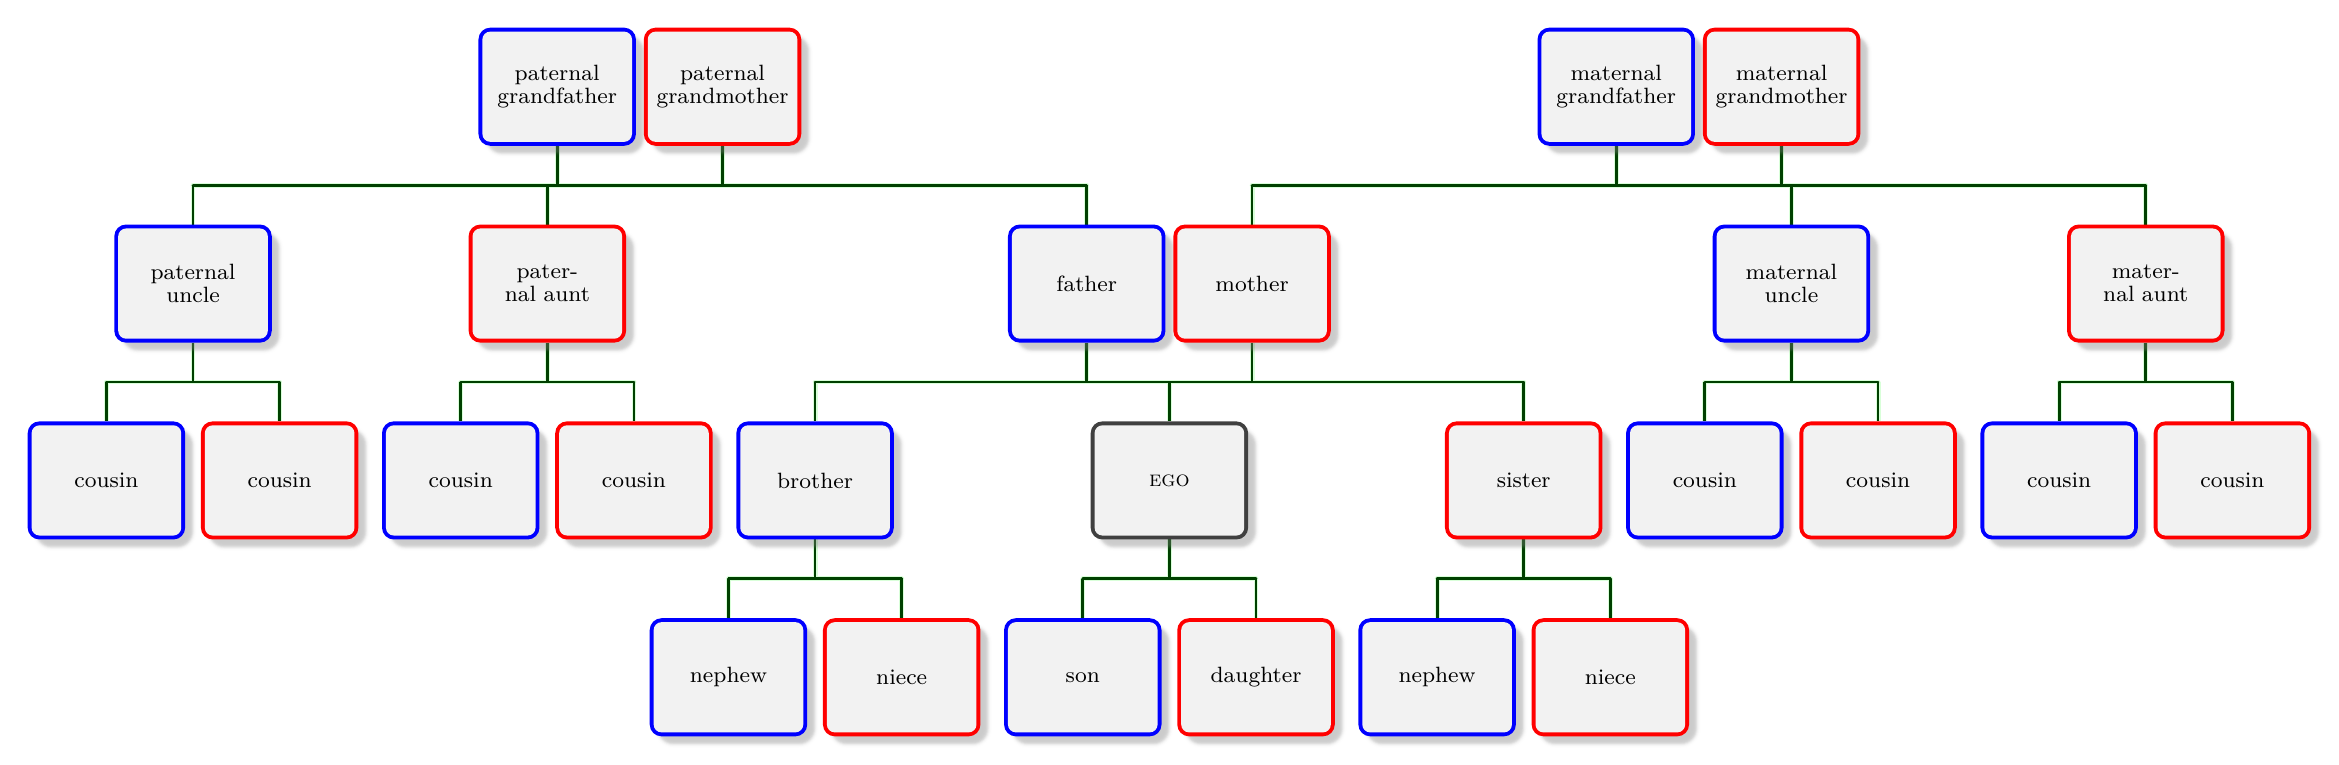
\begin{tikzpicture}
    \genealogytree[template=signpost, id suffix=@p]
    {
      child{
          g[male]{paternal grandfather}
          p[female]{paternal grandmother}
          child{
              g[male]{paternal uncle}
              c[male]{cousin}
              child{
                  g[female]{cousin}
                }
            }
          child{
              g[female]{paternal aunt}
              c[male]{cousin}
              child{
                  g[female]{cousin}
                }
            }
          %OLD WAY
          %child[phantom*]{
          %g[male,id=father]{father}
          %p[female]{mother}
          %c[male]{brother}
          %c{\textsc{ego}}
          %c[female]{sister}
          %}
          %MIRRORED FROM MATERNAL TREE (SEE FIRST IMAGE)
          %child[phantom*]{
          %p[male,id=father]{father}
          %g[female]{mother}
          %child{
          %g[male]{brother}
          %c[male]{nephew}
          %child{
          %g[female]{niece}
          %}
          %}
          %child{
          %g{\textsc{ego}}
          %c[male]{son}
          %child{
          %g[female]{daughter}
          %}
          %}
          %child{
          %g[female]{sister}
          %c[male]{nephew}
          %child{
          %g[female]{niece}
          %}
          %}
          %}
          %}
          %MIRRORED FROM MATERNAL TREE WITH THE TWEAK (SEE SECOND IMAGE)
          child[phantom*]{
              g[male,id=father]{father}
              p[female]{mother}
              child{
                  g[male]{brother}
                  c[male]{nephew}
                  child{
                      g[female]{niece}
                    }
                }
              child{
                  g{\textsc{ego}}
                  c[male]{son}
                  child{
                      g[female]{daughter}
                    }
                }
              child{
                  g[female]{sister}
                  c[male]{nephew}
                  child{
                      g[female]{niece}
                    }
                }
            }
        }
    }
    \genealogytree[template=signpost, id suffix=@m, set position=father@m at father@p]
    {
      child{
          g[male]{maternal grandfather}
          p[female]{maternal grandmother}
          child{
              p[male,id=father]{father}
              g[female]{mother}
              child{
                  g[male]{brother}
                  c[male]{nephew}
                  child{
                      g[female]{niece}
                    }
                }
              child{
                  g{\textsc{ego}}
                  c[male]{son}
                  child{
                      g[female]{daughter}
                    }
                }
              child{
                  g[female]{sister}
                  c[male]{nephew}
                  child{
                      g[female]{niece}
                    }
                }
            }
          child{
              g[male]{maternal uncle}
              c[male]{cousin}
              c[female]{cousin}
            }
          child{
              g[female]{maternal aunt}
              c[male]{cousin}
              c[female]{cousin}
            }
        }
    }

  \end{tikzpicture}
} % end of the resize box


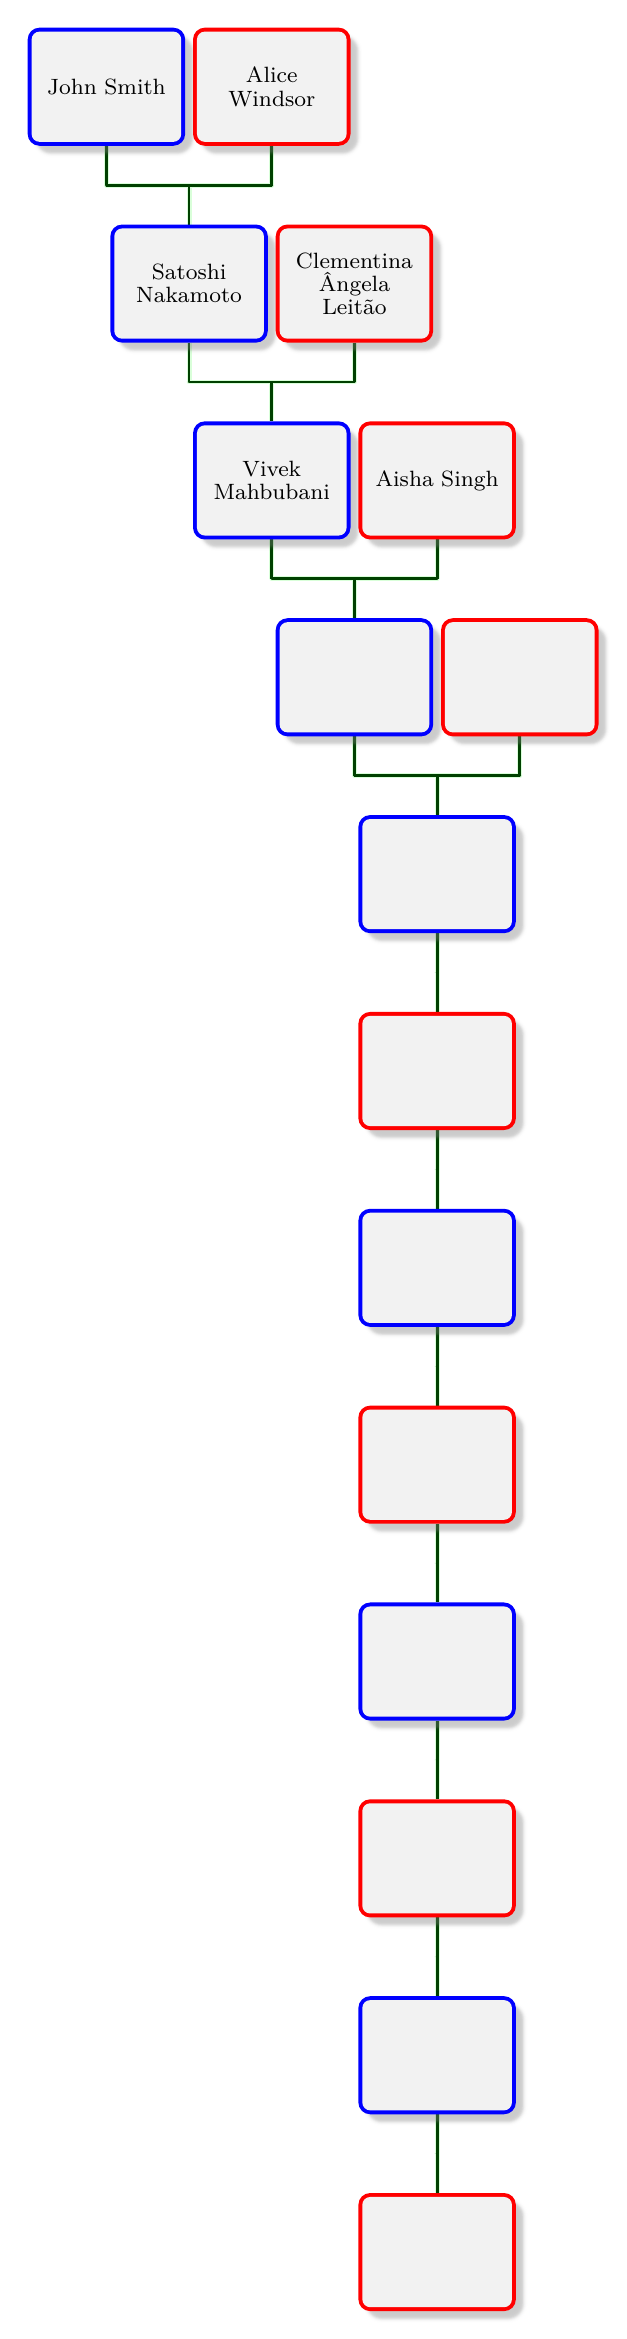
\begin{tikzpicture}
  % Start with the top of the family tree
  \genealogytree[template=signpost, id suffix=@1]
  {
    child{
        g[male]{John Smith} % First generation
        p[female]{Alice Windsor}
        child{
            g[male]{Satoshi Nakamoto} % Second generation
            p[female]{Clementina Ângela Leitão}
            child{
                g[male]{Vivek Mahbubani} % Third generation
                p[female]{Aisha Singh}
                child{
                    g[male]{何鴻燊} % Fourth generation
                    p[female]{陳一美}
                    child{
                        g[male]{李二} % Fifth generation
                        child{
                            g[female]{董英美}
                            child{
                                g[male]{張三} % Sixth generation
                                child{
                                    g[female]{鄧漣洳}
                                    child{
                                        g[male]{彭國} % Seventh generation
                                        child{
                                            g[female]{文家寶}
                                            child{
                                                g[male]{侯泰公} % Eighth generation
                                                child{
                                                    g[female]{廖鹿}
                                                  }
                                              }
                                          }
                                      }
                                  }
                              }
                          }
                      }
                  }
              }
          }
      }
  }
\end{tikzpicture}







% | John Smith |  |  |  |  |
% | --- | --- | --- | --- | --- |
% | Alice Windsor | Smith |  |  |  |
% | Satoshi Nakamoto |  | Smith |  |  |
% | Clementina Ângela Leitão | Nakamoto |  |  |  |
% | Vivek Mahbubani |  |  | Smith 何 |  |
% | Aisha Singh | Mahbubani |  |  |  |
% | 何鴻燊 |  | Mahbubani 何 |  |  |
% | 陳一美 | 何 |  |  | Smith 李 |
% | 李二 |  |  |  |  |
% | 董英美 | 李 |  |  |  |
% | 張三 |  | 李 |  |  |
% | 鄧漣洳 | 張 |  |  |  |
% | 彭國 |  |  | 李 |  |
% | 文家寶 | 彭 |  |  |  |
% | 侯泰公 |  | 彭 |  |  |
% | 廖鹿 | 侯 |  |  |  |

% For this order:

% 1. **John Smith** - `hon`: None, `joeng`: Smith (), M
% 2. **廖鹿** - `hon`: 廖, `joeng`: None, F
% 3. **侯泰公** - `hon`: 侯, `joeng`: None, M
% 4. **Alice Windsor** - `hon`: None, `joeng`: Windsor (), F
% 5. **Satoshi Nakamoto** - `hon`: None, `joeng`: Nakamoto (), M
% 6. **文家寶** - `hon`: 文, `joeng`: None, F
% 7. **彭國** - `hon`: 彭, `joeng`: None, M
% 8. **Clementina Ângela Leitão** - `hon`: None, `joeng`: Leitão (), F
% 9. **Vivek Mahbubani** - `hon`: None, `joeng`: Mahbubani (), M
% 10. **鄧漣洳** - `hon`: 鄧, `joeng`: None, F
% 11. **何鴻燊** - `hon`: 何, `joeng`: None, M
% 12. **Aisha Singh** - `hon`: None, `joeng`: Singh (), F
% 13. **李二** - `hon`: 李, `joeng`: None, M
% 14. **陳一美** - `hon`: 陳, `joeng`: None, F
% 15. **張三** - `hon`: 張, `joeng`: None, M
% 16. **董英美** - `hon`: 董, `joeng`: None, F

% | John Smith |  |  |  |  |
% | --- | --- | --- | --- | --- |
% | 廖鹿 | Smith 廖 |  |  |  |
% | 侯泰公 |  | Smith 廖 |  |  |
% | Alice Windsor | Windsor 侯 |  |  |  |
% | Satoshi Nakamoto |  |  | Smith 廖 |  |
% | 文家寶 | Nakamoto 文 |  |  |  |
% | 彭國 |  | Nakamoto 文 |  |  |
% | Clementina Ângela Leitão | Leitão 彭 |  |  |  |
% | Vivek Mahbubani |  |  |  | Smith 廖 |
% | 鄧漣洳 | Mahbubani 鄧 |  |  |  |
% | 何鴻燊 |  | Mahbubani 鄧 |  |  |
% | Aisha Singh | Singh 何 |  |  |  |
% | 李二 |  |  | Mahbubani 鄧 |  |
% | 陳一美 | 李 |  |  |  |
% | 張三 |  | 李 |  |  |
% | 董英美 | 張 |  |  |  |

% In jyutcitzi this would look like

% | John Smith  |  |  |  |  |
% | --- | --- | --- | --- | --- |
% | 廖鹿 | 廖 |  |  |  |
% | 侯泰公 |  | 廖 |  |  |
% | Alice Windsor 愛麗絲 | 侯 |  |  |  |
% | Satoshi Nakamoto   |  |  | 廖 |  |
% | 文家寶 | 文 |  |  |  |
% | 彭國 |  | 文 |  |  |
% | Clementina Ângela Leitão | 彭 |  |  |  |
% | Vivek Mahbubani |  |  |  | 廖 |
% | 鄧漣洳 | 鄧 |  |  |  |
% | 何鴻燊 |  | 鄧 |  |  |
% | Aisha Singh | 何 |  |  |  |
% | 李二 |  |  | 鄧 |  |
% | 陳一美 | 李 |  |  |  |
% | 張三 |  | 李 |  |  |
% | 董英美 | 張 |  |  |  |

% But suppose the surname Nakamoto 中本, given it can be written as Chinese characters, is taken to be a hon surname, then:

% | John Smith |  |  |  |  |
% | --- | --- | --- | --- | --- |
% | 廖鹿 | 廖 |  |  |  |
% | 侯泰公 |  | 廖 |  |  |
% | Alice Windsor | 侯 |  |  |  |
% | Satoshi Nakamoto 中本 |  |  | 廖 |  |
% | 文家寶 | 中本 |  |  |  |
% | 彭國 |  | 中本 |  |  |
% | Clementina Ângela Leitão | 彭 |  |  |  |
% | Vivek Mahbubani |  |  |  | 廖 |
% | 鄧漣洳 | 鄧 |  |  |  |
% | 何鴻燊 |  | 鄧 |  |  |
% | Aisha Singh | 何 |  |  |  |
% | 李二 |  |  | 鄧 |  |
% | 陳一美 | 李 |  |  |  |
% | 張三 |  | 李 |  |  |
% | 董英美 | 張 |  |  |  |



\section{我哋全部要晒}
我哋唔好再諗「啦咋」嘅「正字」係啲乜嘢。我哋唔好再詏到底係「嗱喳」󱔖、「拿渣」󱔖、「揦苴」󱔖、「揦鮓」󱔖、「藞䕢」󱔖、「\lr{巾}{賴}\lr{巾}{殺}」󱔖、定係「藞苴」。我哋唔好再討論呢啲嘥時間嘅問題。之所以咁麻煩,搞咁耐,同咁難形成共識,個根本問題就係喺個方法嗰度。討論得呢個問題,其實就係問緊「正字」,係字本位主義,係字大晒義忱。被踢出門嘅,唔俾侵埋一齊玩嘅,係詞本位主義,係時文本位義忱。姐係話,問得呢個問題,就係仲係囿於一個「一粒字一粒字」嘅諗法,而唔係「一舊詞一舊詞」、「一舊時文一舊時文」嘅諗法度。

我哋應該脫離「一個時文,一個唐字寫法」嘅教條。「一個時文,一個唐字寫法」本身就係「字本位」思維,跟得多就會字大晒,口講嘅詞彙變成書面上啲字嘅組合。思維嘅會畀字坐咗,而唔係語素。
% 正正就係因為攞字嚟做出發點,所以先至會係「」


我冇興趣同佢哋班哎吔士大夫詏餐懵。佢哋鍾意文人,我哋就\tone{由}{´}得佢哋佢哋思哲\tone{癮}{´},\tone{由}{´}得佢哋爽佢哋嗰鋪易服癖。因為我哋志在嘅,係廣東話榮登世界思哲舞台嘅一日。我哋要嘅,話大事揸𢝵嘅權揸晒喺我哋手,佢哋由´得佢哋󱐂班八婆嘈到天黑啦。

我󱝚目標係愛促進一個發展粵語󱝚新正字法,又同時間保持󱅽同現有粵語文字󱝚尊重連續性。 為󱃡󱜩,我會採用粵切字同粵拼。 點用同幾時用󱝚普遍原則󰳞,就係實詞繼續𢬿漢字黎寫,而虛詞就儘可能用粵切字黎寫。 冇漢字共識󱝚實詞󰳞(名詞、動詞、形容詞、副詞)都會攞粵切字黎寫。 我諗法係,解決󱟡一詞多異寫󱝚單詞󱝚最好符𢝵,𠄡係𢬿過字典󱝚權威或者用本字考黎一錘定音標準化,而係通過類似日文熟字訓所帶黎度󱝚開放胸襟黎畀佢全部同時存在。 就好似「ほととぎす」󱪙日文󰧵可以根據文本的上下文同語域按照作者需要寫做「子規」、「不如帰」、「杜鵑」、「蜀魂」、「郭公」咁,我諗,應該畀作者󱪙「閉翳」共「贔屭」之間去揀,又或者󱪙「揦鮓」、「嗱喳」、「藞䕢」共「\lr{巾}{賴}\lr{巾}{殺}」之間任君選擇。


如果唐字嘅優勢,係在於佢可以捨表聲嚟取表義,咁點解一個時文唔可以有幾隻唔同嘅唐字寫法?點樣寫,就取決於個寫野嘅人佢篇文章啊,佢自己想表達啲乜嘢啊,佢啲naam n
% 用得漢字,就當然有「正字」嘅概念,呢個嘅概念唔係應


\section{蒙古人點做,我哋要比佢哋做得更狠}
你唔好同我講話咩「其實,普通話、廣東話,兩者都識晒,冇咩壞姐」。你噏得出呢句,你唔係腦殘就係奸細。淨係識普通話,就已經經係對我哋廣東話人係危險。一個識聽普通話嘅靚仔,就係一個可以接收到普通話思維同宣傳嘅接毒體;一個識講普通話嘅人,就係一個會講普通話,喺要喺方便同


蒙古人點做,我哋要比佢哋做得更狠。
為抵抗漢人的殖民同化,蒙古人都做出過哪些努力?67年前的南蒙古人提出了以下對策:
一挖:當代蒙古語中不常用的詞彙,優先從古典老蒙文書籍中挖掘
二創:對於實在挖掘不到的新事物,用本民族的語言思維創造新詞
三借:當前兩者都不盡如人意時,直接借用英語或俄語單詞(以英語為主)

廣東話亦當如此
所以我地其實獵巫得係完全唔夠,所有害怕獵漢詞巫嘅都係冇膽匪類同petty叛語者。我地廣東話必須比蒙古語同韓語做得更狠。



\section{消滅詞彙,你擔當得起?}
反對用「智械」
明明已有「人工智能」可以用

長遠應該完全開放新詞發明

個問題係,係咪咩詞彙都可以做新名詞呢?字面意思都未能理解,新明詞≠難理解⋯⋯ 有邊個會去製造一啲難以理解嘅詞彙做新名詞?時代進步幾時都係新+貼地⋯

除此之外,我認為好需要參考使用率,譬如定一個使用下限,當某一個詞輸入達到某個數量,先納入新詞條考慮


係。難理解係非常個人問題,而且好大程度上係領域同個人教育背景嘅問題所致。喺宏觀嘅提高整體語言表達能力嘅目的黎講視野根本不值得理會。你係一個數學家,你發明嘅詞彙文科人睇唔明,so what?又譬如你係一個詩人,發明咗「仙氣」「榮光」「Eyeball」等詞,普通人睇唔明,so what? 況且,根本就冇所謂「睇唔明」嘅現象,亦無可能出現。如果一個詞彙,係有所指嘅,係有實用規則嘅,係可同其他詞彙配搭嘅,咁用用下就會有一定數量嘅人識用,唔識用嘅人都可以學得識。任何話「已經有同義詞」然後話應該對發明新詞採取保守態度嘅人,基本上都係冇參透過喺語言嘅尖端度建模嘅掙扎。只有完全開放詞彙發明嘅語言,先至可以得天下。任何因為文字基建或者語言群守舊嘅語言,都必定滅亡。

你呢段話係完全將我表達嘅嘢,解讀成長你想要嘅意思。其實我個point好簡單:喺add新詞彙嘅時候嚴謹啲去考慮係咪有呢個必要性,定抑或已有其他嘅詞彙或者有更好嘅詞彙替代⋯⋯

而你係解讀成咗似乎我係完全反對開放詞彙㗎喎⋯⋯真係完整咁樣詮釋左為反駁而反駁😅


我冇解讀錯。你係話要考慮有冇必要性。我就係話任何考慮所謂必要性嘅提倡都實際係篩選,姐係反對納某啲詞入紀錄。你自己唔清楚自己想要嘅有啲咩意味姐。

「必要性」根本就係個人情緒選擇。只有全知者先至可能知道喺漫長同浩瀚嘅語言時空裡面一樣野係咪「必要」。人根本就做唔到呢樣嘢。

又好嚴格按照「必要」嘅定義黎討論,如果有一個詞係不必要嘅,佢根本就唔可能出現。佢之所以出現,係因為佢嗰時嗰刻嘅語言時空構成佢出現嘅必要。話其之冇必要,係嚴重缺乏想像力同對語言神力敬畏嘅人先至會講嘅嘢。你話佢冇必要,目的就係要剔除佢—係消滅嘅詞彙啊大佬。消滅詞彙,你擔當得起?

\section{香港人必須放棄漢形名}
香港人必須放棄漢形名,要有自己獨特容易辨認嘅名。

最簡單嘅方法就係 漢字寫English first name + 漢姓 + 漢名

漢姓可以再參考日本喺台灣同韓國做過嘅皇民改名易姓手段,達至去漢化嘅效果。

再顛啲,我哋可以加個「源自地方」好似 “von Hayek”, “van der waal”, “d’anethan”。

介詞可以係英源,用粵切字寫,如「from (夫今)九龍」「of (个夫)蘇豪」

William Chan of Wong Tai Sin Tai Man
威廉陳个夫黃大仙大文
禾子力子央今陳个夫黃大仙大文

\section{嗰啲自然演化出粵切字嘅平行宇宙}
嗰啲自然演化出粵切字嘅平行宇宙,同我地嘅世界其實唔係距離好遠。

粵切字坐正咗,大量好難寫嘅擬聲詞就會即刻雨後春筍咁·氵比么·出黎,之後發展多一輪,就會好似日文裡面嘅擬聲詞,變成為上至首相下至地痞僂儸嘅語言裏面不可或缺嘅詞彙


\section{堅定流?}
我地係特意唔用「流」而用「留」,取音避義。
點解「力久·料」嘅「力久」係「流」?冇任何字典叫我地咁樣寫,但係自自然然我地會咁樣寫。可能係因為我地心裏嘅漢字兆物觀話「力久,同「流」嘅嗰種「不定」係同一個本質,被個水字旁所表達,用「流」就特別符合同有詩意」。但係咁樣其實可以話係污染同干擾,令我地本來要語義分析嘅「力久」多左一層本來唔關事嘅意思要兼顧。

\section{廣東話再上唔到車}
人類嘅科技火車越開越快。廣東話再上唔到車,就會永遠消失。我地其實只需要一本宏大作品,就可以流傳萬世。耶穌講 Aramaic, Aramaic 就得以存活。我地廣東話,有啲咩人講過?有啲咩人係可以二千年之後都有人記得?



\section{我地必須虛心懺悔反省}
我地必須虛心懺悔反省,點解講粵語嘅人,咁多都係思哲不全,言無黹語不法,氣如蠻夷,思緒污穢。

\section{「粵語入文」係一個極度自我鄙視嘅思維模式}
其實,「粵語入文」係一個極度自我鄙視嘅思維模式。佢其實就係文字「官話作主粵作客」秩序嘅呈現,亦係白言文對廣東話嘅根本性歧視同排斥嘅運作機理。
《迴響》裏面有人講過,有「粵語入文」,咁係咪都有「普通話入文」同「英文入文」?
我哋要嘅,唔係咩粵語入文。我哋要嘅,唔係做二房。我哋要嘅粵文,係粵語白話文運動,係文化獨立,係世宗路線。呢個,就係我哋嘅願景,亦係我哋嘅責任。

乜你忍受到「啲」呢個喺廣東話裏面有舉足輕重語法地位嘅詞以普通話嘅「的」加個口字旁嘅方式存在落去咩?乜你忍受到廣東話嘅書面語視覺上呈現住「我哋係普通話嘅變體」係信息咩?乜你忍受到漢字對廣東話喺書面上宣判為方言嘅呢種對待咩?粵語配有自己嘅文字,因為粵語係隻有尊嚴嘅語言。




\section{當一個人同你講「你寫返好啲中文先啦」}

當一個人同你講「你寫返好啲中文先啦」,佢所意味嘅係佢想思哲上殲滅你,但係佢冇料,所以要用埋晒啲󰲎󱂧$_{\text{grammar nazi}}$式嘅旁門左道黎擾敵。此外,佢仲可以藉此打下飛機,覺得自己好勁好好野。「正音」啊「寫錯字」啊「用錯成語」甚至「哦你寫殘體字」(「我話俾老師聽」)都係同樣嘅行為。

可知道,如果你喺英文講同樣嘅野,你係等同犯晒󰠲󰎖$_{\text{faux pas}}$。一個二個會\scalebox{0.5}[1.0]{目}\scalebox{0.5}[1.0]{},因為你好似喺飯檯度瀨屎咁。捉人字蝨係冇󱐡󱝚行為,係對自己身分有自信嘅人絕對唔會做嘅野。

我地嘅語言要昇華,我地就必須杜絕呢種嘅自瀆言辭行為,將呢種嘅污染放逐,令呢種嘅行為變成為言辭上嘅不可以。專注力轉移至語法、詞彙嘅精準、言辭嘅內容複雜性。


如果我哋成功咗,我哋當然可以肯定,我哋而家99\%嘅砌好粵切字喺一千年後全部都會被淘汰,除咗啲考古學家同文學教授識之外普羅大眾冇人識睇—就好似先秦嘅諸夏方塊字,日本平安時代嘅遣遺假名同變態假名,成宗時代嘅古諺文...未來嘅人睇我哋而家嘅粵切字就會好似我哋去睇隸定出黎嘅六國文字—似懂非懂,似曾相識,有一種口噏噏唔出嘅陌生親切感。




\section{論重符「々」}
粵字改革其中一個提議,就係每當用字重複時,唔好咁戇居真係兩隻寫晒佢。我哋可以將後面嘅一隻字用重符「々」代替。呢個用法非常古老,可以追索至春秋戰國啲竹簡。當時通常用「二」,所以亦有人話「仁」字其實係「人人」(以「人」的方式對待「人」)嘅重符縮寫:人人$\rightarrow$人二$\rightarrow$仁。而「々」呢個重符嘅寫法,大興於唐宋。之後畀日本借咗之後就係日本落地生根,變成咗佢地語文嘅一部分。





\section{粵語動漫}
我哋香港,係絕對可以同經濟同文化上需要,將粵語動漫變成為一樣野。我哋必須要通過動漫,將我哋嘅語言唔單止散播同宣揚去呢個地球嘅每一個角落,仲要將粵語殖民到每一個可能宇宙度,等我哋萬世不滅。


\section{粵語動漫}
點解Netflix嘅《末世列車》要有呢一段嘅廣東話呢?原因同點解啲美國大牌子𦧲飯應話BLM一樣:錢。香港人有錢,有國際地位。我哋喺世界萬國秩序度已經有身分。之所以點解模式列車上面有香港人,係因為佢地已經認為香港人,已經係 the 1\%,所以先有錢上到模式列車。

但係只不過咁,香港人呢個嘅身份嘅存在,係危危乎嘅,無時無刻都承受住四方八面嘅威脅。中國想消滅我哋不在話下,其實西方就好似呢個女車長咁,笑騎騎同你講廣東話,但係其實佢維持嘅秩序就係一個你冇得唔用英文應佢嘅秩序。喺佢哋嘅世界秩序,英文先至係王道,粵語嘅地位只不過係畀你地班香港人可以講嗰句「你啲廣東話好咗好多喎—唔駛急慢慢學」畀你自韰一下咁大把。

我哋粵語一定要走日本路線同法文路線—我哋唔需要建立一個類似英語帝國嘅世界流通人口,我哋反而應該將粵語標榜成為高尚嘅象徵,貴族嘅語言,優雅同質素嘅標誌,使人將粵語就聯想起氣派、原則、精闢嘅精神同意象。英文,個個都識,故此係臭西。日文、法文,要擺錢投資先至識,係上流社會嘅標誌。粵語,必須咁樣走。

\section{不切實際論、冇可能架喇論 全部 其實 都係 求其反對論}
「不切實際」
「冇可能架喇」
「香港係華夏正統」
「唐詩點算」
「廣東話好好地用漢字有咩問題」


以粵切字改革粵文,脫離漢字文字政權,奔向諸夏,畀香港獨立





1. 講啲特別哽耳嘅說話,另佢哋太難受,另佢地講「唔講廣東話」同埋「講普通話」同「唔係香港人」概念上掛鉤。要另佢哋喺香港感覺「異化」,被排擠,不受歡迎。譬如:
- 「你邊度人黎架?講普通話。」
- 「香港人唔講普通話㗎咯~」
- 「唔講廣東話邊忽係香港人?」
- 「香港唔歡迎普通話」
1. 有權用嘅就要特別對待用普通話嘅人,刁難佢地,服務差啲。濫權都要。譬如:
-
1. 見到有人喺公眾場合講普通話,要另佢哋唔舒服,可以:
- 鬧佢、
- 騷擾佢
- 錄影佢
- 直言用「支那」、「殖民者」、「蝗蟲」開口鬧
- 肢體驚嚇佢:如果佢食緊M記,上前推冧晒佢啲嘢。





新造字

風申/丰申 phone
甲申app
扁糸 print
卜手 book
昷定 run
勞申 load
黎忄like
吞辵 ten3 (本字理應為「退」)
Link 寧手/寧糸
Prefer
Preference

Form
highTo 舀
The 羍
In 兗
So 蘇
That 躂
With 业乎
Of 咢、咢乎
for 沎
From 虖壬/冘
En- 恩-
-ment 璺/忞/門/亹/悶 (加於動詞後,將其動詞名詞化虛化,以表達高一層的概念):
-tion 純 (使用於部分並列結構的動詞,以及後,表示虛化以表達高一層的概念): representation 代表純
-ary/-ery
-ness 弥斯 瀰
-Chy 亓
-er 儿、儞
-ly
-y 漪
-ium 烎
-al 奡
-ality 奡之忑 (唔要)
-ity 茌,之茌
-ence 艮,艮斯
-ism 依忱,之忱,忱。依意. 意忱
義忱、意忱  (理論、論述)
依忱  (主張)
現忱  (現象)
-ist 依忱者,士,依忱士。依意者,
-ive 枼
-able
-ize 厓斯、淣斯 施、斯、貰
En- 摁
-able 也圃
-tic 忒 克
Sub-
-pseudo
-faux
-quasi
-dom 丼
-hood 乎特
Under 奀打
In
On
At
Or
And
Anti-
Un-
In-
Non-
Meta-
Under-
-fy
-ing 營








\section{英文可以做得我哋嘅,廣東話就係。}






\section{convinced}
I was beginning to be convinced but now I am utterly convinced. That Cantonese must have spaces, like Korean. The calligraphic issue must give way. For the space itself is a grammatical marker that marks the beginning and the end of a word. This tool of demarcation will allow poet and playwright to invent new words by putting words together within the confinements delineated by the spaces between words. Written Cantonese needs all the tools imaginable for it to revitalise and resurrect its lost vocabulary. A Hebrew -esque recycling off ancient words for purposes anew is the way to go. But we can’t do that if we can’t tell if this is a new word because we can’t tell if these  characters familiar so and so sequenced are merely a fanciful poetic playful arrangement or other mark of the invention of a new word, where a familiar noun is turned into a verb or verb is turned into an adjective or an adjective is now henceforth interpreted as a noun in this particular context.

我啱啱開始被說服,但而家完全信服。粵語書寫必須要有空格,正如韓文咁。書法嘅問題必須讓步,因為空格本身就係一個語法標記,標示一個詞語嘅開始同結尾。呢個劃分嘅工具可以畀詩人同劇作家透過將詞語拼埋一齊,喺詞語之間嘅空格劃定嘅界線內,去發明新詞。書面粵語需要所有可以想像嘅工具,去振興同復活失落嘅詞彙。好似希伯來文咁,將古詞回收再利用,用於全新嘅目的。但如果我哋唔能夠知道呢啲字係咪新詞,我哋無法分辨呢啲熟悉嘅字符排列係純粹玩味嘅詩意遊戲,定係創造新詞嘅標記,喺呢個特定嘅語境入面,名詞變成動詞,或者動詞變成形容詞,又或者形容詞從此變成名詞。






粵文要有空格


% \chapter{其他腍審野}


\section{吳語小字對簡體字嘅立場}
如果你去睇下啲用吳語小字去構建吳語書面語嘅文嘅話,會見到佢哋基本上係一律否定同排斥中共簡體字嘅。但係,佢哋會喺某啲位選擇使用異體字,譬如用「躰」唔用「體」咁。呢個選擇好明顯係完全唔係因為字義原因,而係因為美感原因。佢哋想喺呢度郁.大必.々.嗰度郁.大必·々,以達到一種同漢字官白文有難以言喻嘅距離—操作同效果就好似日文中嘅漢字咁。我哋好大機會都要做啲類似嘅野。



\section{女書嘅故仔}
呢個故仔我自己第一次睇到嗰陣真係喊出黎。話說喺1982年武漢大學嘅一位宮哲兵博士生喺湖南一個叫永江嘅小鎮度發現到呢隻文字,仲發覺成個鎮只有女人識呢隻字,故此叫佢做「女書」。點解淨係得女人識呢?因為男尊女卑,女人冇得讀書,只可以靠撞靠估偷偷摸摸攞男人用嘅漢字,以其漢字讀音書寫自己嘅野,通常攞黎寫日記、繡喺扇同手巾仔上,記載嘅通常都係佢哋盲婚啞嫁、老公打老婆、姊妹情嘅哀詩。有人認為,女書可能有至少150年歷史,因為有啲天平天國嘅錢幣上有女書。而喺文革嗰陣,大量大量數之不盡有女書嘅用品全部畀人破四舊燒晒。

女書嘅自然傳人,即係細細個就寫女書大,有自然女書觸覺嘅人,喺2009年辭世。女書,已經冇自然傳人。


東亞有好多嘅文字演變都係咁,男人用漢字,新嘅、地位低下嘅、低劣嘅新文字,就由女人發明、使用、傳承。日本嘅假名,係好大程度上由啲貴族冇得參政嘅女室,為咗證明自己都可以搭嗲講到文學而自己演變出黎;韓國嘅諺文喺成宗發明咗之後冇幾耐就被一眾儒士所拋棄咒罵,但因為已經流落咗民間,女性就攞佢黎用,咁就傳承咗600年—而諺文正式上台,係要等到20世紀日本帝國將韓國嘅王帝同儒家全部殺晒,先至開始抬頭。

我成日都話,我地,係喺呢個漫長嘅六百年旅程嘅開端。係,係六百年。係好長,好痛苦。但係,係會成功嘅。係一定會成功。我地,就係喺呢個漫長嘅六百年旅程嘅開端。



\section{「方言」呢個狗牌}
當我地叫一樣我地認之為存在嘅「事物」為乜乜,賦予佢名稱時,我地從中係會奠定咗我哋對佢嘅認知,並確立咗我哋對佢存在嘅信念。而好多時候,呢個名字同佢係社會嘅用法,會衍生會維持某種政治或權利架構。呢個名字亦可能未必能夠「真實」「確切」反映到被描述物嘅現實特點。簡單啲黎講,就係我地叫某樣東西為X,我地就不由自主地認定咗X嘅存在,以及其存在模式。

咁講咁多同「方言」一詞有咩關係?如上所述,我地稱得一啲嘢為「方言」(同一啲嘢為「非方言」嘅物體),我地已經認定咗「方言」嘅存在,並且喺潛意識上奠定咗「方言」同「非方言」嘅標準。但係到底「方言」同「非方言」嘅界定線係啲乜嘢?係咪肆意無由(arbitrary)?而且就算呢個分類係人為嘅,係構建出黎嘅,佢有冇用?好唔好用?係可以擴大人類嘅知識,定係其實會導致人類概念模糊?用呢個詞黎剖釋世界,有冇咩政治同權力組態嘅衍生副作用?

先(試)處理一下「方言」呢個概念。我喺呢度我唔再以問題引渡,直接慳啲時間講小弟點睇算。

首先要講嘅「方言」一詞,無論喺大眾嘅觀點之中,抑或喺大中華學術界中,呢個詞語所表達嘅概念都同「dialect」有啲出入。雖然中西學術交流已經使到兩者逐漸趨同,但從其者在學術中所產生的蛛絲馬跡,我們仍然可以見到兩者有異。

「方言」同dialect嘅共通點就係佢地都係描述緊某種同「語言」相對嘅語碼(code)現象。呢個係釐定「方言」同「語言」嘅出發點,亦係普羅大眾對呢兩個詞嘅普通理解。

但係好明顯呢個理解係冇辦法自立,根本就自相矛盾,而且只要一直堅持「方言」同「語言」係相斥嘅關係,就必定無辦法成為一個內部邏輯通順嘅語言詮釋範式(interpretative paradigm). 原因好簡單,因為「語言」language 一詞,普遍概念上包括咗「方言」dialect嘅概念。你可以諗諗,方言如果唔係語言嘅一種存在形式,咁佢係啲乜野?如果「語言」嘅定義係「一個以人類口頭發聲按著某種邏輯規律以傳達信息資訊嘅系統」,咁「方言」又豈能不是一種語言嘅一種存在形式?

之所以會出現以上嘅類悖論情況,係因為我地冇釐清呢個同「方言」相對嘅「語言」嘅概念係啲乜東東。事實上,茲「語言」不同彼「語言」。

「方言」始終喺我哋日常嘅理解當中係相對於「語言」。我地好多時候講X係「語言」而唔係「方言」,言下之意可能係指X按某種標準而言比較「正式」;反之,當我地話X係「方言」而唔係「語言」,言下之意就係X「(唔夠)正式」。

用以上對「語言」同「方言」嘅理解,如果講得抽象同哲學一啲,就係當咗「語言」同「方言」係「一位謂詞」(1 place predicate).

有時候我地又會以以下嘅方式去演繹。我地可能會話X係Y嘅方言,而喺呢種講法係Y係「語言」,X係「方言」,而「語言—方言」係一種階級關係,Y(語言)支配住X (方言)。例子包括今日講到滿城風雨嘅教育局偉論:「粵語係漢語方言」。政治上冇咁具爭議嘅例子就可能有:African American English 係英文嘅方言/ Canadian French 係法文方言 / 北京話係官話方言 / 四邑話係粵語嘅方言 / Bavarian 係德語嘅方言。

但仲未完。有時候我地又會以以下嘅方式去演繹。我地可能會話X係C嘅方言,而Y係C嘅語言。例子:Spanish 係西班牙語言而 Catalan 係西班牙方言 / 普通話係中國語言而粵語係中國方言。

以上兩者都係將「方言」當為係「兩位謂詞」(2 place predicate):前者係「語言—方言」嘅兩位謂詞 Rxy where x 係方言 y 係語言;後者係「語言/方言—地方」嘅兩位謂詞 Rxc where x 係某種語碼,c係地方,而x係方言定係語言就視乎x係乜同c係乜。

到呢度「方言」呢個概念有咩問題應該已經可以略見端倪。好明顯,以上三個對「方言」嘅詮釋,係冇可能同時並立嘅。(呵呵我相信用以上嘅定義可以用數學證明出黎,但而家就唔搞呢範野啦)。

第二個問題就係以上三個嘅詮釋,都係只可以釐清「語言」同「方言」嘅關係,但係冇畀任何指示我地去決定咩時候咩係語言咩係方言同咩係咩嘅方言。簡單而言就係我地仲係冇釐定語言同方言嘅實質標準。

姑勿論以上三個詮釋明顯會要求有三個不同嘅標準呢個問題,就算我地暫且只專注求祈一個,我地都會發覺,個標準好難定。點解?因為有好多例外,同好難得到「普遍性」同「泛可用性」。呢個問題其實唔係好複雜嘅姐,但係要講就真係好煩水蛇春咁長,一句既之曰其理則為「語言只不過係有軍隊嘅方言咁解」。而正因茲原因,語言學家普遍都唔會嚴格定義「方言」係啲乜東東,只會當「方言」一詞為rule of thumb 速語,唔會胡亂定性乜乜語言為「方言」或「語言」 。

好啦,到戲玉啦。到底點解「方言」一詞有問題?

請循其本—我地開頭就講咗,我地社會用語中嘅詞彙同用法,係可以塑造我地對現實嘅理解。標籤某一種語碼為「方言」,係可以(亦幾乎必定會)產生龐大嘅政治作用,而呢個作用往往係具壓迫性,打壓性,同賤貶性。使用「方言」一詞黎稱呼同標籤某種語碼,就係會使被標籤者馬上蒙受語言權威同威望(prestige)嘅損失,而往往他者嘅損失,就係某者嘅(政治、經濟、文化)得益。例子實在太多,中國內對粵、吳、客、閩諸華語、法國對 Occitan, basque, 西班牙對 Catalan, 等等。

以上嘅原因適用於dialect同埋「方言」,但「方言」一詞就更加有問題。「方言」一詞除了包括晒dialect嘅絕大部分潛意思之外,佢係仲額外承載住濃郁但難以言喻嘅大中華思想同中華中心主義。呢個好複雜,難以詳述,但小弟盡下力。第一,「方言」一詞歷史上係相對於「雅言」,而雅言就係天朝上國嘅語言(口語)。所以按呢個邏輯,家下天朝上國嘅雅言係普通話,所以粵語、吳語、客家語等等就通通都係「方言」。呢個邏輯體系以前仲比較強,而家就已經弱,但係始終係普羅華人大眾中仍然有無色無聲嘅影響。要知道,喺清末民初搞翻譯書院嗰陣,藏語、蒙古語、粵語、甚至英語、法語、日語,都列為「方言」。梁啟超當初讀西方邏輯嗰陣,唔知係乜,都挾硬將「邏輯」一學列為「方言」。

二、西方嘅dialect同(standard) language嘅普羅釐定界線,唔係「相互可通性」mutual intelligibility, 就係國界。中國嘅「方言」除了一向兩者,仲包括文字。如果個語言用得漢字,就係「方言」。所以按呢個邏輯,即使北京人去上海去香港去潮州去台南聽唔明上海話廣東話潮州話閩南話,佢地都係會話佢哋冚把爛係方言。在極端啲嘅連日文,甚至歷史上用過漢字嘅韓語同越南語都唔放過話係方言。

以上兩點加埋「方言」一詞所可以帶來嘅政治作用,應該足夠說明點解「方言」茲詞理應慎用。




\section{囻之語音}

\ruby{囻}{󱼒}之語音
今日,十月九號,係諺文日。

諺文日,又稱之爲「韓字日」({\koreanfont 한글날}),係南韓爲咗記念喺1446年,世宗大王公佈《訓民正音》({\koreanfont 훈먼정음})而定嘅國定假期。

北韓都有自己對應假期,定喺一月十五號。

之所以要咁大陣象舉國慶祝,係因為「諺文」嘅發明,解決咗朝鮮呢個國家嘅文字問題,事關喺諺文之前,韓國係冇自己嘅文字。諺文嘅發明,唔單止為韓語嘅「有音無字」「言文分離」提供咗解決方案,奠立咗「韓文」嘅基礎,仲為韓國奠基咗佢哋自己嘅獨立文化嘅基礎。如果倉頡係華夏文明嘅開端,話諺文係朝鮮文明嘅開端都唔係冇得拗。

\subsection*{諺文嘅發明背景}

「諺」嘅原意係「俗語」,顧名思義「諺文」一詞就係「表記俗語(朝鮮語)之文字」嘅意思。呢度其實都已經見到諺文嘅發明開端。

嗰陣時,韓語只不過係平民百姓嘅口語,貴族同士大夫雖然口講韓語,但係寫嘅就係漢字。想寫野,就必須用漢字。用漢字,你可以寫文言文。如果想將篇文言文用韓語讀返出黎,就要用一啲非常複雜、無咩系統嘅規矩,去將文言文句子轉化成為符合韓語語法嘅句子,先至得。如果你想寫韓語,姐係想「我手寫我口」,你淨係有漢字可以用。你就只可以用漢字,攞住漢字嘅音去寫韓語,亦即係通篇用「假借」嘅手法去寫,好聽你就係《萬葉集》,難聽啲你真係同「港女文」冇乜分別。而呢啲嘅查實係見招拆招嘅書寫手法,就衍生咗所謂嘅「鄉札」、「口訣」、「吏讀」。漢字本身要學就已經成本高,噉樣嘅文字秩序就令韓文嘅讀寫變得更加係難上加難。

朝鮮國嘅第四代國王世宗大王,好想喺佢嘅國家推行儒家禮教,但係佢寫用黎教育大眾嘅書,淨係可以用漢字,庶民根本睇唔明。佢嘅臣民,有野想講,都冇辦法喺書面上同佢表達。為咗解決呢個極度嚴重嘅「言文分離」問題,佢就下令要發明一隻新文字。喺《世宗原詔》度,佢話(原文係漢文):
\begin{quotation}
  國之語音,異乎中國,與文字不相流通,故愚民有所欲言,而終不得伸其情者多矣。予爲此憫然,新制二十八字,欲使人人易習便於日用耳。

\end{quotation}
用粵語白話文講嘅話就係:

\begin{quotation}
  我哋國家嘅語音,同中國嘅唔同,所以同中國嘅文字唔啱牙。正因為係咁,愚民(唔識字嘅平民)就算有野想講(有冤情),最終好多都冇辦法同國家申訴。我為呢個問題深感悲哀,對佢哋面對嘅情況深感憐憫。所以,我而家就整咗二十八個新字出黎,希望人人都可以好容易學識,畀喺佢哋日常生活度攞黎用。
\end{quotation}

世宗大王發明嘅諺文,都真係相當之驚為天人。呢隻文字,表音奇準,使用規則奇簡,字符同字符之間喺字形設計上有耐人尋味嘅隱性邏輯,仲將中國「天地人」同陰陽學說暗合咗入去,仲借鑒咗漢字嘅六書原則並加以闡發托展——基本上前無古人,後無來者。同樣係漢字衍生出黎姊妹書寫系統,比如西夏文、女真文、喃字、方塊壯字、日本假名等等,都冇諺文咁科學——諺文稱之為東亞文字最為犀利者實在當之無愧。

呢隻文字,真係「智者不終朝而會,愚者可夾旬而學」。意思姐係「聰明人唔使一個朝頭早就可以學識,就算係白癡都可以十日內搞掂」。

\subsection*{反對諺文同戀慕中華嘅士大夫}
世宗嘅諺文推出咗冇幾耐,就有人出黎大大聲聲反對。最有代表性嘅,就係一個叫崔萬理嘅儒家士大夫。佢寫咗一篇題為《反對創建韓文》(又名《上疏反對世宗推行諺文》)畀世宗睇嘅上疏。裏面開宗明義就話:
\begin{quotation}
  我朝自祖宗以來,至誠事大,一遵華制,今當同文同軌之時,創作諺文,有駭觀聽。儻曰諺文皆本古字,非新字也,則字形雖倣古之篆文,用音合字,盡反於古,實無所據。若流中國,或有非議之者,豈不有愧於事大慕華?
\end{quotation}

我哋唔使翻譯晒出來都睇到佢嘅反對重點,就係「採用諺文,就係脫離中國,咁樣係違反『一遵華制』、『至誠事大』、『事大慕華』嘅國策。」乜嘢係「事大」呢?「事大」,姐係「事大主義」。「事大」一詞來源於《孟子》嘅「以小事大」。。「事大」裏面嘅「事」,可以理解為「服侍」。「事大」就係「為大行事」或者「服侍個『大』嘅野」。咁乜野(或者邊個)係「大」呢?就係中華,亦姐係中原皇朝,亦姐係中國。而「事大主義」注意,就係外交政策上視中原皇朝為中華(故此為「大」),以自己為「小」,而呢個外交政策上嘅體現,其中一部分就係文化上靠攏中國,將自己變成為「小中華」。崔萬理嘅意思就係,如果推諺文,就係違反朝鮮作為小中華嘅身分——言下之意就係,做得中華,就一定要用漢字。

佢之後又話:

\begin{quotation}
  自古九州之內,風土雖異,未有因方言而別爲文字者,唯蒙古、西夏、女眞、日本、西蕃之類,各有其字,是皆夷狄事耳,無足道者。《傳》曰:「用夏變夷,未聞變於夷者也。」歷代中國皆以我國有箕子遺風,文物禮樂,比擬中華。今別作諺文,捨中國而自同於夷狄,是所謂棄蘇合之香,而取螗螂之丸也,豈非文明之大累哉?
\end{quotation}

簡單黎講,就係話自古以來,就算方言唔同,都唔會改用其他文字(換句話就係佢認定韓語只不過係方言)——而唔用漢字嘅,就係自作夷狄。由華夏文明去開發夷狄,令佢哋變成為中華,就係古而有之嘅大道理姐;調返轉頭本來已經喺華夏文明裏面,跳返出黎做野蠻人,邊有咁嘅道理架?之後佢又話朝鮮好耐之前(春秋戰國時期)就已經有中原嘅「箕子」蒞臨,朝鮮仲繼承咗佢所帶黎華夏文化添
——我哋嘅文化,根本就可以同中華有得揮。家下你另起爐灶發明諺文,係放棄中國而將自己化為冇文化嘅野蠻人,係放棄蘇合呢種香草嘅香,而換黎曱甴卵嘅行為,噉樣仲唔係文明大倒退?

\subsection*{諺文之後嘅發展}

崔萬理$_{\text{fi li fe le}}$$_{\text{bi li baa laa}}$嘅理性批鬥,都唔係好阻止到世宗大王推行諺文。諺文好快就喺民間度流出去散播。但係唔係個個都接受同肯採用。開初大部分嘅名門望族同士大夫多對諺文嗤之以鼻,繼續用佢哋嘅漢字,要到二十世紀上流社會先至出現啲毫無系統嘅漢諺混寫。諺文就反而喺低下階層,尤其是係女人同奴婢之間度廣泛採用。唔少本來唔識字,亦唔會有機會識字同寫野嘅人,就攞住諺文黎寫日記。
但冇幾耐,諺文就畀人$_{\text{ban}}$咗。

朝鮮國嘅第十任國王燕山君,係一個大暴君,專搞埋晒啲寸斬、炮烙、拆胸、碎骨飄風等等嘅酷刑。而且佢又淫蕩非常,後宮膨脹,又時不時將啲佛寺改建成為妓院。百姓民怨沸騰,淨係得把口就用諺文寫野侮辱同詛咒佢。燕山君就下令取締諺文。而自此之後,諺文都主要淨係喺婦女同僧侶之間流傳使用,故諺文亦稱為「女書」或者「僧字」。

呢個情形一直到十九世紀末、二十世紀初朝鮮半島民族意識強烈提升先致開始有改變。大韓帝國高宗國王喺1894年至1896年間推動甲午改革,其中一部分頒布命令規定「法律條文與公文基本上應採用諺文;但全漢字或漢字與諺文混用的版本於必要時可以增加」。之後冇幾耐日本帝國夾硬吞併韓國嗰陣,日本人頒發咗《朝鮮教育令,規定埋一個星期中韓語同諺文嘅教育時數》(但韓語同諺文係冇官方地位),亦編製咗「詞根用漢字,虛詞用諺文」嘅韓文教科書。但係到第二次世界大戰開戰,諺文就被視為係朝鮮國族主義嘅象徵,又事被禁止使用。

諺文嘅下一個歷程碑,係1948年政府提出嘅《諺文專用法》。自此,韓漢混寫就真係抬頭。到咗六七十年代,極力主張使用諺文嘅總統朴正熙,喺1970年發表漢字廢止宣言,小學冚把爛廢除漢字教育。到咗1980年代中期,韓國嘅報紙、雜誌等,開始逐漸降低漢字使用頻率。噉係因為幾乎冇接受漢字教育嘅世代(諺文世代)開始佔多數,搞到漢字嘅出版物賣唔出——漢字續漸安樂死。

與此同時,北韓做咗自己嘅諺文拼寫改革,亦一刀切完全廢除晒所有漢字;中國改用簡體字,二簡字唔成功要打倒褪;星加坡曾經試過自己簡化漢字,但用用下就直接採用中國嘅簡體字方案快靚正;台灣、香港、澳門就繼續用繁體字;越南完全廢除漢字,採用以法文為參考基礎嘅拉丁拼音文字發明咗「𡨸國語」(chữ
Quốc ngữ);而日本就繼續漢字假名混用。

而到咗近年,漢字教育喺南韓仍然係教育政策嘅一大爭議。有人認為廢除漢字造成嚴重文化斷裂,搞到韓國人連《世宗原詔》同自己嘅憲法都睇唔明。廢除漢字亦導致韓語無法攞自己嘅漢語詞根發展新詞彙,社會同經濟發展所需要嘅新詞彙只可以全部透過音譯英文呢種嘅烏呢媽叉手段黎解決。唔識漢字,亦令韓國同中國、日本、台灣等地文化交流上出現隔膜,甚至因為同音字問題而搞出「賤出名將事件」。但亦有人認為,漢字「三多五難」,而且而家諺文已經完全成熟,學漢字根本就多餘同嘥時間。況且,諺文咁鬼犀利,咁鬼精準,點解要學人地國家(中國)嘅野?最大力反對漢字教育嘅「韓字學會」甚至話「韓字係可以喺全世界面炫耀嘅科學文字」、「漢字係特權階層嘅反民主文字」、「根本就冇南韓國民認為韓字專用唔方便」。呢種嘅心態同朝鮮民族主義結合,都滋生咗唔少語出驚人嘅說話,譬如咩「韓國之所以可以科技發展一飛沖天係因為諺文奠定咗韓國嘅數學同邏輯基礎」。到咗而家,漢字復用喺南韓仲係處於一個唔嗲唔吊嘅狀態。

\subsection*{諺文畀粵語嘅啟示}

我哋而家嘅粵語,仍然處於一個未能夠全面「我手寫我口」嘅落後境況。「本字考」仍然係處理粵語「有音冇字」嘅主流方案,以拉丁字母為基礎文字嘅粵拼亦有其推廣——但呢啲嘅手法其實都係自己嘅問題同盲點。「本字考」嘅基礎理論同方法論其實非常可疑,生產解決方案龜速,而且毫無系統,民眾參與唔到。而且本子考完全係事後解決主義,係社會度有咁上下數量嘅人用一個詞,我哋先至會搵個本字出黎,故此追唔上民間粵語嘅高速發展,甚至係排斥自然發展。其實呢度已經見到本字考嘅方法論謬誤——如果個詞係新嘅,《康熙字典》裏面又點會有本字呢?咁樣唔係刻舟求劍係乜野?所以話呢,本字考其實係延續住粵語言文分離嘅劣況,雖然有陣時佢哋都生產到啲雅味不俗嘅方案,譬如「齮齕」(gee
gut)、「䒐䒏」(忟憎),同「𪘲牙聳䚗」(依牙鬆鋼)噉,都咪話唔話有聯綿詞嘅feel。


至於拉丁拼音方案,字型美感上同漢字相斥,即使全民識用,都冇人會當作為正式文字。除非我哋用極其粗暴極權嘅手段全面廢除漢字,將漢文粵語完全消滅打殘,將粵文構建成果推倒重來,喺呢個一片荒蕪嘅曠野度畀粵語全面採用粵拼,否則粵拼就只會係類似普通話拼音嘅輔佐子系統。外國人或者香港嘅少數族裔學咗粵拼,其實都會依舊係文盲,因為根本冇野係用粵拼寫。

韓國廢除咗漢字,其實可以話係個陰差陽錯嘅偶然,而唔係佢演化嘅必然結果。漢字好似已經喺韓國徹底死亡,但其實不然,佢仍然有復活嘅機會——只要政治環境風向改變,基本上係必定會復活,因為好似崔萬理嘅士大夫喺韓國依然存在。漢韓混用,反而先至係最自然同效益最大化嘅方案。所以,我哋應該從諺文歷史度專注嘅,唔係漢字嘅死亡,而係諺文點樣完成咗「韓語有韓文」個工程。更重要嘅,廢除漢字然後諺文專用所損失嘅,係比唔上唔用諺文夾硬用漢字寫韓文嘅荒謬。

「{\koreanfont \ruby{감사합니다}{󱢮󱍖󱪪󰻦󰣖}}」當然唔夠「感謝{\koreanfont 합니다}」咁多資訊啦;「{\koreanfont 안녕하세요}」(「安寧{\koreanfont  하세요}」)、「{\koreanfont  죄송합니다}」(「罪悚{\koreanfont 합니다}」)、「{\koreanfont 미안합니다}」(「未安{\koreanfont 합니다}」)、「{\koreanfont  실례합니다}」(「失禮{\koreanfont 합니다}」)等等嘅例子都睇到漢字嘅表意同跨語言溝通功效啦。但係我哋要對比嘅唔係「諺文專用」同「漢諺混用」,而係「諺文專用」同「漢字專用」。如果呢乍野全部用漢字寫,噉啲「habnida」點算呢?用「合尼大」假借黎寫?如果用漢字假借黎寫韓文會覺得係篤眼篤鼻嘅,噉點解「多謝曬」裏面嘅「曬」我哋又唔覺得係問題?呢個「曬」,無論你係用「曬」又好,「晒」又好,個詞都係同個漢字冇意思。你用漢字,反而係隱藏同模糊咗粵語嘅語法部件。同樣道理,「做咗」「做緊」「做埋」「做過」「做住」「做親」「做做下」嘅「咗、緊、埋、過、住、親、下」其實全部都係攞咗漢字黎做啲漢字唔應該做嘅野。

更重要嘅係,我哋香港人因為我哋嘅政治成見同我哋引以為傲嘅文化背景,好容易無視咗漢字教育,真係需要巨大成本。要民眾學漢字,你係要投入大量資源同事件架。雖然我哋會覺得喺依家呢個世代,呢啲錢同事件根本唔係啲乜野。但係諺文發明咗之後幾百年黎都冇政府支撐,都可以喺低下階層繼續傳承發展,反而漢字就無法擴張佢自己嘅領域,就已經暗示住邊一個嘅成本效益比較好。我哋因為愛戀漢字,所以抗拒所有漢字以外可能可以解決到我哋語言寫唔出嘅方案。某程度上,我哋係寧願保住漢字,粵語唔可以原汁原味我手寫我口都冇所謂。再簡單啲黎講,我哋個個都係崔萬理。

廣東話,配有自己嘅文字。粵語,配有自己嘅文字。我哋,配有自己嘅文字。
所以,要粵字改革。

央乙·止子·丩丐·丩百·亾乇·禾会·
亾丐·夫丂·〡〧〩·乃千·〡〇·央乙·〩·央乜·



% \chapter{語言同思維}

\section{粵語係一個冇哲學嘅語言,甚至乎係一個不善於畀人用黎討論高階思哲內容嘅語言。}
粵語係一個冇哲學嘅語言,甚至乎係一個不善於畀人用黎討論高階思哲內容嘅語言。


香港人亦有一套用廣東話音系同語音直覺去同化同粵化英文詞語嘅潛系統,用之於英文名之上就會出現港式英文名。



我肯定他朝有日粵人一定會有人說:「我們自古以來就是天朝最忠誠地添煩添亂的蠻夷,陳炯名是我們偉大的民族英雄,其身承蒙自趙佗和冼夫人那抗命不屈、誓要獨立的大粵國靈,本來勢必建國,完成大粵人民二千年來的刺秦偉業。
% 


\chapter{Epigrams}
The state language is the language of politics and government. The national language is the language of lovemaking.


I often think English monolingual speakers know nothing of the joy of speaking one’s language, because they’ve never known any other language, and they do not know the full range of capabilities and incapabilities of the English language. They therefore use words most uncarefully. They speak but do not say things. Not because



A paradigm is a comprehensive interpretation system of facts.

An ideology is a paradigm coupled with commandments.




Why the Cantonese, with her cuisine so alike with the Japanese in talent and delight, fail to match them in worldly sophistication in the eyes of the peoples of the world?








We the Cantonese connect with each other by speaking extraordinarily loud, angrily, red facedly, and aggressively, over the dinner table filled to the brim with food


\section{我哋嘅子彈}
每隻講出口嘅廣東話時文,都係一粒解放香港嘅子彈。
% \chapter{美感}

\section{美感絕對不是主觀的}

美感絕對不是主觀的,這是極度懶惰的相對主義。美觀是有邏輯的,否則不可能出現漢字圈一致認為殘體字醜死的現象。

你說推廣粵切字比推廣英語難。這是false的,嚴重直線邏輯,也完全機理錯誤。你根本完全沒有讀清楚我寫的東西。懂不懂英語根本不關事,問題在於拉丁字母的語文構建是逆民意和逆漢字語文美感的。粵切字反而是順民意和順漢字語文美感的,或至少沒有拉丁字母這麼嚴重。

你第三點也是完全不關事。他們傾慕英國文化,不意味一個漢字和拉丁字母混合的文章會雞犬升天,更不意味一個全拉丁字母的粵文會被他們學習。反而,用拉丁字母的粵文,所享受的尊重會更加低。是四不像。

粵切字設計上已經完成,短期上不會再改,因為暫時沒有任何的空間或需要改動。群眾開始使用後,理則出現新發展空間,就反而可以再調整。但重新設計是不會出現的。

所以呢,正字派係完全且永遠解決唔到文言分離,粵語語文構建不全,我手寫唔到我口嘅問題。po1根本就係「棵」嘅白讀音。但係呢度就有人唔小心得意得濟,「搵」(發明)咗個本字出黎。
本字考係非常好玩,發明過程令人陶醉—問題唔係在於發明,而係個發明過程不成系統,內無理則。文法仿效語法,故此語法必須係建基於有理則嘅文字上,繼而理則地呈現出黎,文法先至會相繼承語法,變得有理則。而當文法有理則,語文先可以有邏輯。


% \chapter{普通話}

\section{講普通話係殖民嘅行為}
講普通話係殖民嘅行為。大義凜然仲要大條道理叫囂畀人歧視根本就係腦入水。唔係冇事就手足有事就蝗蟲,係發現原來我地信錯人,根本就唔係真係同我地企喺同一陣線,亦唔係真係同我地同心同德。佢只不過係透過香港黎凸顯自己係超級中國人。佢覺得有權喺香港講普通話,冇可能唔知個殖民性。姐係話,佢根本就只不過係兜個圈但之後都係殖民咁解。

唔好講到佢好hurt. 佢畀人窒唔畀講普通話,香港人日日如是,呢樹要同你講英文嗰樹同人講普通話,一黎個自價不菲嘅中國人就要即刻遷就轉台香港人都未嗲,邊度輪到佢嘈?仲有,死咁多人,佢呢啲雞毛蒜皮嘅野搞到滿城風雨,佢仲好意思?

我自己係非常非常想世界各地嘅人同我地行埋一齊,但係咪覺得你同我地行埋就好巴閉好大支野要乜都包容。粵語係香港嘅語言,而且應該係至尊語言。你入黎香港人無任歡迎,但唔好妹仔大過主人婆客家當地主。好煩。好討厭。


我地必須日本化,做到日本已經成功做咗嘅之餘,我地仲要超越佢哋。我地要成功將我地嘅文化發展到班鬼佬同大陸人仆崩鼻過黎崇拜我地同加入我地,要佢哋為自己可以講到粵語而自豪,要令佢哋自願同興高采烈咁摒棄自己嘅語言,就好似班入日嘅Gaijin淨係講日文咁。我地仲要令到佢哋自己嘅圈子都內部講粵語,就好似好多honkies abc 同喺英國讀書得耐嘅香港人自己圍位都會講英文。



因為絕對冇好處。唔玩呢個遊戲,只會俾人覺得你冇了,你廢,你玩唔掂先至喺度發爛渣。輸者無抗議之直。呢個現象一直都冇徹底打破: 抨擊姨得最犀利嘅,不外乎胡適嘅「八不主義」、 五四嘅新文化同新文學運動嗰陣嘅文風新倡議,同埋毛澤東主張嘅「大眾文學」。雖然股民同文言已經係所有一個需要用語文推進發展嘅範疇中被白話文所取代,但係呢種嘅引經義忱沒而不歿,陰魂不散,揮之不去,仲係死纏爛打。之所以係咁,有所以由官話演化出嚟嘅「白話文」再次有文言分離嘅跡象,漸漸演變成為「白言文」。

引經義忱最揦脷之處,就係佢驅使同鼓勵,趨逳啲引經言忱越嚟越難名,越嚟越難拆,唔搞到你𢱑晒頭都唔放棄,引嘅經典越刁鑽就越顯得你學識淵博,用嘅詞越難讀越睇唔明月冇辦法望文生義就越顯得你思考深邃。引經言忱,咁樣催生左一種秘語言忱:引經義忱秘語義忱。

秘語義忱天下就係一個用舊語主宰今事嘅義忱。喺呢個義忱之下人會變得思哲上不誠實,唔老實,爽韰為上,真想義理遺下。人只求得到嗰一下嘅韰,同埋自己身邊群組嘅認同:到底有冇道理,有冇玄理,有冇義理,話叉知佢。而正正因為咁樣,冇晒動力去以個人,獨立,新穎,批判性嘅視覺去剖析事情。冇新嘅言忱,冇新嘅意忱,冇——嘅義忱,一切都係舊酒新樽。賦予墨水靈魂嘅唔係真、實、啱、確,嘅玄理同玄義,而係死念。墨水都變得污穢。

懶醒,懶而不醒,就係一個清醒同誠實有勇氣凝視真理嘅人睇嗰個上海妹妹引用《鄭公克段於鄢》個鋪嘅唯一結論。


我地講粵語嘅,離不開漢字、漢系語、同漢經典嘅魔咒。其中一個一直抑壓住我地思維嘅最可惡魔咒,就係「反問」。

我地成日用反問,因為我地嘅語言驅使我地去用反問。我地幾乎語言上冇法不用反問黎釐清或說明我地嘅觀點或道理,因為(1)我地嘅詞彙缺乏抽象理想概念嘅詞,或者嗰啲詞口噏出黎硬係有啲古怪,好似個語言唔畀我哋講嗰啲關乎玄義價值嘅野—講野取易不取難,所以個個就口噏噏都係用反問你帶出自己嘅觀點同道理;(2)我地嘅語言習慣(陋習)已經形成咗,冇特別嘅意識去作出改變;(3)所謂嘅經典同先賢都用反問,一直缺乏理則嘅運用,具體嘅邏輯,截卒嘅論證,我哋想拾人牙慧都冇,而且如果我地嘗試直接論證,某程度上就會係違反已經成立咗同根深蒂固已成嘅論證文化,係唔埋堆嘅表現。

我地一定要有意識地抗衡呢種嘅語言陋習。我地唔好再反問,要直接說明。

反問嘅運作原理,就係要從問題引申出一個情感或理則演繹,而呢個情感或理則演繹最後會衍生出一個邏輯結論,而呢個邏輯結論係要係自悖,或不符一般普遍不予質疑嘅理念,繼而逼使思題者接受嗰個自悖嘅邏輯嘅否定。

由此可見,反問係一個非常之迂迴嘅論證方式。但係佢唔單只係迂迴其實佢亦都好低效率,成功率亦都唔係非常之差同低保證,論證質素亦非常之唔得掂。

首先,反問係一個問題, 人面對問題第一個嘅反應唔係去進行嗰個理則演繹,而係直接答咗個問題佢,咁我哋想要嗰個效果就冇咗啦。第二,你要得到嗰個自悖嘅邏輯,係要通過一段嘅邏輯演繹,但係可能人哋自己本身有其他嘅先設命題,而呢啲命題會影響理則演算嘅吞吐品,導致佢得唔出你想要嘅邏輯自悖結論。

說服力方面,反問作為修辭嘅小手法,其實冇乜野,但係問題就係在於反問(至少喺漢系語言裏面)有一種自韰嘅效果,容易導致一用反問就一發不可收拾。試問如果你喺度聽一個人演講,佢一輪嘴咁不停咁同你提出問題,仲邊有時間消化同進行以上嘅理則演繹?所以反問嘅重複使用,甚至濫用,係會導致說明嘅道理越來越膚淺、越黎越忽視細節:因為只有咁樣嘅命題或道理先至可以被反問所拉倒出黎畀人睇,深入啲高深啲嘅論證就係咁先。而正正因為咁,所以最後尾都係有理說不清,稍微唔思哲上完全死蛇爛鱔嘅人就會唔擺呢個邏輯,不歡而散。

我地要直接說出真理,唔好兜圈,唔好反問,要直接洗對家腦,否定同排斥反問主義,養成好嘅語言習慣。

% \chapter{英文}

\section{英文呢種語言}
英文呢種語言真係有一種容許其實根本乜嘢都唔識思想紊亂概念混淆嘅廢柴顯得自己好似好有料事事看得通透嘅神奇力量。
\chapter{Wiki 唐字討論整理}

\section{命名問題 (2007年)}
最新留言:3 年前
31則留言
5個人參與討論
漢字呢個名係日本呢啲地方叫,表示係外來字。響中國地方,叫字就夠囉。中華民國就叫國字,香港就叫佢中文字。好似係近年先至流行叫漢字。HenryLi 2007年3月5日 (一) 12:25 (UTC)

改中文字都好呀。--WikiCantona 2007年3月5日 (一) 14:51 (UTC)
反對改。中國內地本身就係叫漢字。中國大陸、韓國、日本都叫漢字。「字」同「漢字」唔同,字嘅範圍大啲。而「中文」係一個模糊唔科學嘅世俗叫法,好似「廣東話」「中國話」呢啲叫法噉。--我哋越人 2007年3月8日 (四) 08:09 (UTC)


% \section{對2007年命名討論嘅討論}
% 根據Special:diff/657162,本身呢篇文喺2012年5月18號之前係叫「漢字」嘅,係喺2012年5月19號先畀人搬版搬咗去「唐字」,所以上面講嘅「唔好改」係保留「漢字」唔改。同後來嘅討論唔同,𠝹番開先。
% 仲有,明明2012年之前嘅討論得咁少,當中根本就冇討論出搬去「唐字」嘅共識,無啦啦就搬咗版。咁嘅操作真係……Well,苦笑。--Cangjie6 (傾偈) 2021年8月22號 (日) 16:52 (UTC)
% @Cangjie6、H78c67c、Z423x5c6、Detective Akai、SC96、Deryck Chan、Pokman817:你地睇返上面嗰次討論,2012年搬文嗰次討論有3個人參與,有1個人係明顯反對(User:我哋越人),有2個係支持(Henry、WikiCantona)。再睇返近日嘅Talk:黑膠唱碟#原創研究成分,有1個人——User:Kowlooner係明顯反對,有2個人係明顯支持(特克斯特、Akai)。喺參與討論人數嘅情況根本同嗰次(2007年嗰次)一模一樣,呢2次(黑膠唱片+2007年漢字討論)嘅討論大家都係畀咗理由 而唔係盲目投票玩票數,再加埋User:WikiCantona喺呢到講嘅:Special:diff/1671405(唔係大多數支持就ok),已經充分證明嗮2012年嗰次搬文夠係未符合「大多數」情況,同Talk:黑膠唱碟嘅根本一模一樣(都係2對1嘅情況)。2個人支持用「唐字」就可以搬文(1人反對),2個人支持用「黑膠唱片」就唔可以搬文(1人反對)??
% 如果W君視咁多粵維常客嘅討論同揀用字嘅理由方面係操控票數、投票認為「漢字」係更好選擇就係同化同破壞粵維嘅行為(即係User:Cangjie6話嘅「污名化」大家粵維常客),咁我呢到都可以當你喺黑膠唱碟文章自把自為、濫用權力,喺唐字文章唔跟返討論意見堅持搬文係雙重標準。
% 喺下面章節嘅討論,大家都睇到W君喺被主流意見反對下講咗粵維一直唔用「投票」嚟決定,但係呢次參與基數唔係4、5個人同非活躍用戶咁簡單,再加埋「Special:diff/1671405(唔係大多數支持就ok)」,佢個句「大多數」呢三隻字嘅意思又一次自打嘴巴(自己言下之意都證明咗大家去決定用邊隻字係冇問題,唔使畫公仔畫出腸 寫明一定唔可以用「投票形式」 但係最尾討論結果其實係基於「大多數用戶意見同留言」去決定,咁樣佢只係喺到偷換概念),有導向(符合WP:NOT#DEMOCRACY嘅原則)、有理由、唔係盲目投支持同反對,呢啲意見理應聆聽,去睇下下面討論「大多數」用戶覺得邊隻字用字更準。
% 憑乜嘢Henry搬返返去?Henry都有責任出嚟解釋,一係WikiCanona喺黑膠唱碟亂嚟(包括禁止非管理員搬文又係,吳君如音樂作品畀人搬咗2次 次數同黑膠唱碟一模一樣,又係有人反對,又唔見你鎖文?又喺到玩雙重標準?自把自為,唔怪得喺Wikipedia:城市論壇_(政策)#個別案例嘅處理問題一路遊花園 講埋啲偏離話題嘅嘢 User:Cangjie6有興趣去食花生都可以望下)。
% 我就建議User:Cangjie6喺粵維活躍少少,唔係長遠落去會趕走嗮啲人,對呢到發展唔好,亦都學Akai喺Talk:拉爾夫史坦曼呢到咁講:你好意思同我講「羅馬都唔係一日起好」(嗰到佢哋2個討論緊點解粵維開張15年呢到都係咁少人肯入嚟寫文,User:Cangjie6都知道點解呢到一直都咁少人肯入嚟啦)。特克斯特 (傾偈) 2021年8月23號 (一) 16:12 (UTC)
% @特克斯特、Cangjie6:有理由懷疑WikiCantona同Longway22係以為自己係呢到嘅地頭蛇,加上十幾年嚟從未有人質疑過佢地既做法、或者做埋啲同佢地背道而馳嘅野,令到佢地自把自為,隨隨便便就打擊異見者。另外,最先話要投票既人係Dr.Greywolf(「我不嬲都嗌開「漢字」。投票囉。Dr. Greywolf (傾偈) 2021年8月21號 (六) 14:58 (UTC)」),唔係我,Dr.Greywolf絕對有責任出嚟講返野,但佢居然叫人地唔好再ping佢,明顯係怕事同埋唔負責任。Akai 博士 (傾偈) 2021年8月24號 (二) 03:50 (UTC)
% 關鍵在於中段時最後akai閣下嘅(總結提出voting表決壓制討論)做法、即正式總結將成個未有確切成投票採樣案嘅議程,包裝成一個投票案甚至係一個絕對壓制少數意見嘅決議案,先至係最為打壓少數異見嘅做法,請幾位認真考慮幾位依家嘅做法係咪繼續製造不公同其他問題,唔好兜著人多勢眾系度模糊幾位經已明顯違反一般討論同辯論嘅群狼做法 Longway22 (傾偈) 2021年8月24號 (二) 04:02 (UTC)
% @Longway22:由2007年嘈到依家,嘈左接近十幾年,十幾年都未有結果,你係咪要諗下呢個問題呢?跟據Wikipedia:請求移動響英維嘅解釋,有一種情況係唔畀搬文(「A title may be disputed, and discussion may be necessary to reach consensus」),明顯呢篇文響2012年同埋2021年嘅討論已經唔適用呢個條例,單係Henry響2012年嘅搬文已經係唔啱。Akai 博士 (傾偈) 2021年8月24號 (二) 04:40 (UTC)
% @Longway22:其實我最初唔係好想搞投票,只不過見有絕大部份既維基友都支持用漢字,但反對既目前只有幾個,而呢篇文已經由2007年爭議到依家,不如直接投票嚟個一刀兩斷。我好希望可以停止一個長達十幾年嘅爭議。Akai 博士 (傾偈) 2021年8月24號 (二) 04:46 (UTC)
% 呢點並冇改變閣下經已造成嘅後果,即使閣下提出表面合理嘅理解,同時亦係未有解決當下爭議同擴大咗程序問題等衍生風險,請閣下一併考慮埋同適時中止風險嘅繼續 Longway22 (傾偈) 2021年8月24號 (二) 05:18 (UTC)
% 如果要唔好擴大程序問題等衍生風險,噉係咪應該首先改正番錯誤嘅程序先講得通?即係將2012年呢一次錯誤嘅搬版更正番,還原番去「漢字」先。-Cangjie6 (傾偈) 2021年8月24號 (二) 06:53 (UTC)
% @Longway22、Cangjie6:我發現Longway22淨係識得針住我既意見,但未有反思自己亂咁指控人嘅錯誤,又唔去諗下點解咁多人支持用漢字而唔係唐字;當Cangjie6、特克斯特提出要搬文,Longway22亦未有回應兩位嘅意見,反而一直玩針對、恃住自己係少數人就要求大部份人聽佢既意見,以為自己受到不公平既侍遇,但事實係Longway22一直堅持己見、未有企響其他人嘅角度去諗;粵維非常多文章內容都好少,但我見到Longway22成日都響同人嘈,好少見佢有認真寫文,如果佢將同人嘈嘅精力放響寫文到,相信可以對粵維貢獻更多;而我認為我既做法即使唔係響維基常用,亦唔覺得會引起好似Longway22所講嘅咁大風險,投票就算唔啱響討論入面用,但面對一篇嘈左接近十幾年都未完既文,可以睇到討論已經解決唔到問題,因此響呢個時候,投票係唯一選擇。Akai 博士 (傾偈) 2021年8月24號 (二) 07:26 (UTC)
% 所以本案經已係嚴重違反多個經已提出嘅問題同規程、但係以上由akai帶起嘅幾位根本唔當一回事,十分遺憾,本編保留依家由於akai帶起大陣仗嘅相對少數異見位置。唔再重複。 Longway22 (傾偈) 2021年8月24號 (二) 08:25 (UTC)
% 我唔覺得會引起大陣仗;另外,如果跟規程,咁呢篇文章響2012年嘅搬文咪一樣唔符合規程。好心Longway22嘈少啲野,執多啲文啦。Akai 博士 (傾偈) 2021年8月24號 (二) 08:46 (UTC)
% 呢輪興用「屈」。User:特克斯特閣下,唔係話!我2007年明明話用「中文字」,嘩,你都幾叻個喎,覺得我能夠預知未來,2007年根本都冇人提過「唐字」。咁又入我數啊,仲有,2007年 User:我哋越人係反對「字」或「中文字」。五年之後(2012年)先有人搬去「唐字」(可能係第三個出路),當時冇有人反對?再過三年後,2015年又有人提再搬,討論直到而家。就算你講黑膠碟嘅點人數情況係正確(又只係講咗啲唔講啲 - 不盡不實,麻煩你收返無理指控),根本完全就係兩回事。User:特克斯特閣下對之前嘅事仲係耿耿於懷,咁麻煩你返去處理緊嘅地方,繼續講你嘅觀點啦。--WikiCantona (傾偈) 2021年8月24號 (二) 11:11 (UTC)
% @WikiCantona:哈佬你終於又響度出現啦;咁你認為2012年,搬去「唐字」是否符合規程?發表你既高見Akai 博士 (傾偈) 2021年8月24號 (二) 12:18 (UTC)
% @Detective Akai: 喂,哈佬,你都好忙下,又寫嘢,有傾過唔停。冇法啦,又有人「捩橫折曲」,唔出嚟唔得。我呢啲地頭蟲,高見就唔敢啦,不過,「符合規程」你可唔可以澄清下先?2012年嘅英文規程?2012嘅呢道嘅慣常做法?因為近年嘅做法?--WikiCantona (傾偈) 2021年8月24號 (二) 12:30 (UTC)
% 跟據Wikipedia:請求移動響英維嘅解釋,有一種情況係唔畀搬文(句子「A title may be disputed, and discussion may be necessary to reach consensus」),即係如果篇文(響搬文前)係對命名有爭議嘅話,咁就要加{{Move}}或者經討論後先至搬文,明顯2012年嘅搬文係未得到反對者嘅同意,即係響冇共識既情況下搬文。唔知WikiCantona、Cangjie6、特克斯特同唔同意Akai 博士 (傾偈) 2021年8月27號 (五) 08:55 (UTC)
% 首先要多謝 User:Detective Akai 閣下,「同意」同「唔反對」唔係一樣。「共識」係咪要得到每一個人嘅「同意」?定係每一個人都「唔反對」、「唔出聲」就得呢?可以深入討論,不過,不過操作上,「唔反對」會啱呢度些少。吓吓要啲討論人,返去表態「同意」,唔係人人有興趣/想噉做,共識就好難。例如「黑膠碟」嘅討論,閣下你唔出聲,User:特克斯特閣下都覺得有大致嘅共識。2012年嘅情況,要 2007年 User:我哋越人反對搬版,你知啦呢度啲用家神龍見首不見尾,流動人口多,要搵返佢問佢同意,可能有啲難度。直接搬咗先,睇吓有冇人反對,都唔係一個唔可行嘅做法。最重要嘅係,2012年搬版呢味嘢,真係各有各做,其實到而家都係(好少少)。所以你有興趣賞面都去 Wikipedia:城市論壇_(政策)#搬版,改名嘅本地框架再商議傾下。--WikiCantona (傾偈) 2021年8月27號 (五) 09:50 (UTC)
% What,之前WikiCantona唔係一直話要有共識既咩。Akai 博士 (傾偈) 2021年8月27號 (五) 09:54 (UTC)
% 係,冇錯。近年我眞係覺得共識緊要。現實係 2012 年嘅嘅情況唔同,我就係嗰陣時嘅情況作出一啲評論?!--WikiCantona (傾偈) 2021年8月27號 (五) 10:38 (UTC)
% 唔明WikiCantona講呢個說話既理由,冇記錯我多次見到WikiCantona響討論頁提出要搵共識。Akai 博士 (傾偈) 2021年8月27號 (五) 11:47 (UTC)
% @Detective Akai:閣下,當有兩個有你冇我嘅意見時,而兩方都企得好硬,(除非一方讓),共識嘅形成係冇可能。所以好多時會退而求其次,喺兩個冇辦法妥協嘅方案之間,搵第三條出路,第三個選擇。黑膠碟嘅討論就係呢個情況,黑膠碟係黑膠唱片同黑膠唱碟嘅第三選擇。當然我哋可以要求每一個有份討論嘅人都要「同意」呢個選擇,實際上係幾難。不過,只要討論嘅人唔再提出反對(唔出聲),會 easy 啲。咁大致可以睇成有共識。希望噉解釋,可以清楚少少。2012年「唐字」嘅搬版,亦用咗呢個唔出聲就即係唔反對嘅原則。因為噉,2012年 User:HenryLi 閣下搬版之後冇人反對。所以喺呢個細維基嘅運作,水靜河飛嘅時候,都唔係一個唔實際嘅做法。 --WikiCantona (傾偈) 2021年8月27號 (五) 12:07 (UTC)
% @Detective Akai:Akai醒少少先啦,喺黑膠唱碟嗰陣都係同一個月份內討論,同2012年User:Henry Li喺冇人留意嘅情況下搬文類比唔到(User:Cangjie6都認為要返返去初版;W君喺呢到自己都識得講)(2012年「唔出聲就即係唔反對」亦都係唔係你喺呢到回應大家搬文冇問題原因、打圓場嘅講法,要留意依家所有規則之類全部係佢自己up 龍門任佢搬)。回歸呢轉討論,仲有兩方都堅持,咁就要睇下多數參與討論者意見係用邊個,其他2位嘅,頂多符合User:SC96講嘅「各自表述」(Special:diff/996178),PQ77wd當年搬文手法同佢哋2個今次嘅手法一模一樣。特克斯特 (傾偈) 2021年8月27號 (五) 19:17 (UTC)
% @Detective Akai: 哈哈,「Henry Li喺冇人留意嘅情況下搬文」,嘩,特記(親切啲唔再稱呼做閣下),好嘢,你係全世界啲人心裏面啲蟲?定係 super AI?又知道2012-2015年之間冇人留意到?2015年有講嘢啦,三年之後。「打圓場嘅講法」,都眞係希望化解矛盾。話啲 rules 由我噏出嚟?噉 Akai 閣下睇吓我講得有冇道理啦?最後,特記有講User:PQ77wd當年搬文,我都想知多啲,不如去Wikipedia:城市論壇_(政策)#搬版,改名嘅本地框架再商議講下(唔知鍾意搵嘢嚟拗嘅特記一定唔會去?)--WikiCantona (傾偈) 2021年8月27號 (五) 22:45 (UTC)
% @Detective Akai、Z423x5c6、Cangjie6:同上情況,又係佢唔認數就齋講「呢輪興用「屈」」。至於,「咁麻煩你返去處理緊嘅地方,繼續講你嘅觀點啦」,喺黑膠唱碟呢篇文已經明顯有咗共識係用「黑膠唱片/黑膠碟」呢兩個寫法,點都唔會係「黑膠唱碟」,係閣下仲喺道扮揾唔到共識唔去搬返去「黑膠唱片/黑膠碟」,我唔似閣下喺「Talk:唐字」咁樣「繼續講你嘅觀點啦」,咁樣同死撐唔尊重共識冇分別。至於Akai講嘅「地頭蟲」我會返Wikipedia:申請做管理員/Z423x5c6嗰度講。特克斯特 (傾偈) 2021年8月25號 (三) 22:28 (UTC)
% 有冇係我新嘅資料 update 呢?亦都講咗,揀一個題目名,有多個因素要考慮。如果將共識純粹睇成多數 vs 少數,閣下根本就冇興趣傾,唔想搵妥協嘅方案,「死撐」呢啲字對個討論冇乜幫助啵。--WikiCantona (傾偈) 2021年8月27號 (五) 09:53 (UTC)
% 「「死撐」呢啲字對個討論冇乜幫助啵」,因為要學User:Z423x5c6咁講,話要做有意思嘅討論,你先前攞嗰啲資料已經畀佢全部反駁嗮,亦未符合User:Cangjie6嘅意見(睇清楚佢提倡嘅嘢先好繼續拎資料出嚟)。唔話「死撐」,你會繼續喺度留言對住空氣講野,自己以為自己仲係同Z423x5c6等用戶有效回應個問題同參考資料,咁先最冇幫助(人哋明明嘅意見都係用「漢字」說服唔到其他人用「唐字」)。仲有如果共識唔包「多數 vs 少數」(喺充分討論下 唔係齋投票 呢次凝聚共識當然唔係齋投票了事),如果繼續唔認數,呢啲亦都係直接違反共識嘅明顯證據,亦都未讀透Wikipedia:共識。特克斯特 (傾偈) 2021年8月27號 (五) 19:17 (UTC)
% 今次我已經盡量避開無謂拗撬。哈,你都唔係第一次,你講嘢聽落有汶有路,最叻就係講啲唔講啲 - 不盡不實 - 避重就輕。對住你真係唔知好嬲定好笑。我話共識唔係純粹睇多數對少數,你就話「如果共識唔包「多數 vs 少數」」,真係豎手指公,啲邏輯都冇。「喺充分討論下」家下未有,「唔話「死撐」,你會繼續喺度留言對住空氣講野」,嘩,好嘢,原來有人唔回應我嘅觀點,又係我錯!喺 WP共識「編者都應該作出善意努力」,我就做緊啦,幾鐘頭之前先至 upload 咗張相,討論「漢字」嘅可能性,我會繼續提出,有如果真係有誠意嘅話,去傾吓。--WikiCantona (傾偈) 2021年8月27號 (五) 22:45 (UTC)
% @特克斯特:嘩,我瞓個覺姐,討論已經多左咁多...,我想講,WikiCantona並未提供一個合理解釋畀我。如果跟足維基規舉做野,共識係好重要,元維基都係咁講。另外,「唔出聲就即係唔反對」,佢冇出聲你點知佢唔反對(笑)?Henry響2012年既搬文,明顯係違反左Wikipedia:請求移動,係未有共識,唔應該搬文;我唔理有冇人留意。總之我目前仲見到WikiCantona係未承認多數人支持「漢字」既結果。我想多口問一句:當初Henry響兩人支持、一人反對下都可以搬文,咁點解依家係九人支持、兩人中立、三人反對既情況下,就唔可以搬文呢?Akai 博士 (傾偈) 2021年8月28號 (六) 00:57 (UTC)
% 我都好想知道點解。而且,而家大家發覺當年嘅搬文咁有問題,對比桑切斯(暫名)呢篇文,哪怕呢個名唔符合粵音,但係產生改名爭議後,WikiCantona都搬返去呢個名先,嚟繼續討論。係噉,點解而家呢篇文又唔係用同一種做法,搬番去「漢字」先?-Cangjie6 (傾偈) 2021年9月3號 (五) 11:48 (UTC)
% 要答答 @Cangjie6:先,其他嘅仲寫緊,畀啲時間我。桑切斯係畀 User:Detective Akai 加點同加長個名,我搬返轉頭,拎走個點,令一位 User:特克斯特唔同意,再反轉,我用管理員嘅身份,改返做原名,為嘅係唔好有編輯戰,轉頭討論,唔關「符合粵音」嘅事。之後,為咗大家舒服啲,亦交畀其他管理員搞。呢篇嘅情況,原則係「討論開始咗就唔好搬版」,英文維基百科嘅規矩,近期喺 Talk:墨索里尼度,因為我以用街坊用家嘅身份,玩佢搬兩次我搬兩次,後來 User:Detective Akai 閣下話,論開始咗就唔應該搬版,講得有道理,聽佢話,我自己搬返去 Detective Akai 閣下搬完之後,有人提出反對,嘅名「貝尼托·墨索里尼」。同呢度比較相似。
% User:Detective Akai 閣下講:「當初Henry響兩人支持、一人反對下都可以搬文」,User:Detective Akai 閣下可能係嚟自未來世界(笑),所謂嘅「支持」係 2017,2015年。2012年 HenryLi 搬版,你最多話當時冇人反對,唔通 HenryLi 有時光機,知道後來會有人「支持」佢?!嚴格咁講, 佢當時冇人支持,亦冇人反對。2007年嗰「一人」係反對搬去「字」同「中文字」,唔通佢預知未來 ,知五年後會搬去唐字,「反對」定未來。所以你句說話超乎事實,結論亦唔合理。
% 所以,希望搵到個雙方面都可以接受嘅辦法,先郁都未遲。--WikiCantona (傾偈) 2021年9月4號 (六) 04:10 (UTC)
% @WikiCantona:2007年既討論明顯係未有共識;Henry亦響搬文個陣冇提出任何理據。依家大多數人都係支持用「漢字」,好似係得以WikiCantona為首既人唔肯承認,響度死賴。Akai 博士 (傾偈) 2021年9月4號 (六) 10:22 (UTC)
% 咁根本就係雙重標準——有啲文即使未有定名共識,但係發現搬版違規,就首先搬番去舊名(哪怕舊名有問題)先繼續討論。而,而家呢篇,就聲稱要「搵到個雙方面都可以接受嘅辦法,先郁都未遲」。噉樣雙重標準法,叫人點接受?點服人?
% 所謂「雙方面」,就只不過係閣下憑偏見一直極力要用假古董,而好多人認同要用「漢字」呢個共識係好明顯嘅。係咪只要唔啱閣下心水,閣下就有權用「玩規程」而夾硬黎講,最終粵維就係聽閣下你支笛?
% 仲有,而家呢篇文係HenryLi喺2012年違反規則擅自搬版嘅,而HenryLi違反規則搬版唔係第一次。睇到島嘅編輯歷史,喺2016年,佢又係冇討論結果就擅自搬去洲,畀殘陽孤俠鬧佢:「身為管理員更加唔應該知法犯法未經討論就改名。」然後到咗2018年,HenryLi無啦啦又再擅自搬版,而殘陽孤俠再還原、再鬧佢:「請唔好再用一百幾十年前嘅標準來規範宜家嘅文章。」點解島呢篇文畀HenryLi違規破壞後,可以噉樣即刻還原番,但係漢字唔只唔還原,仲要有明顯共識都仲繼續唐字落去?而家粵維係咪興玩雙重標準?-Cangjie6 (傾偈) 2021年9月4號 (六) 04:21 (UTC)
% 命名問題 (2012年畀人搬咗去「唐字」之後)
% 最新留言:3 年前
% 16則留言
% 5個人參與討論
% 我呢個土生土長嘅香港人,聽過「中文字」,聽過「漢字」,就係冇聽過「唐字」。我唔認為粵文維基百科應該故意標奇立異,違反大眾嘅約定俗成叫法。無論改做「中文字」定「漢字」,我都贊成,就係反對叫「唐字」。Cangjie6 (傾偈) 2019年10月12號 (六) 21:34 (UTC)

% 反對改。最新論述可以睇下底。——Longway22 (傾偈) 2019年10月13號 (日) 03:48 (UTC)
% 反對改,睇下底嘅參攷。--WikiCantona (傾偈) 2021年8月21號 (六) 06:46 (UTC)
% 反對反對改,見下低。--Cangjie6 (傾偈) 2021年8月21號 (六) 14:18 (UTC)
% 反對。依家廣東話用字,甚至文法、字音,都一直畀強勢語言蠶食緊。戰後大批外省人走難到香港,佢哋已經以民國教育嗰套,代替咗原來廣東人用字。學校都日漸畀依啲人所控制,無聽過有乜咁出奇。學校迫人用「書面語」。無學校教育,而大家從來唔睇唔學廣東話嘅文學遺產,又點會知?以前教書嘅人叫做「先生」,後尾嗰啲國語為中心嘅,逐漸改晒「老師」。咁樣,細路長到大人,可以一世都未聽「先生」咁叫法。長此下去,無「糖水」、只有「甜湯」。無「生菓」,只有「水果」。無「片」睇,只有「視頻」。只「吃」無「食」,只「喝」無「飲」。廣東話用字並無靠山,若果只係自己閱歷淺未聽過,從來唔回顧傳統,廣東話真係危危乎。只要清洗落去,廣東話用字,只係國語、普通話翻版,頂多「的」改為「嘅」,「是」改為「係」,咁依度開來又有乜意思?依度開來就承傳廣東話文化用意,而唔只翻版國語、普通話。HenryLi (傾偈) 2021年8月23號 (一) 01:27 (UTC)
% 反對樓上嘅反對。但凡活生生嘅語言,一定會keep住有變化,只有已經死咗、放入博物館嘅語言(例如哥德語)先至會唔變,一隻唔變嘅語言絕對唔係咩好事。唔係凡變化都關畀人控制乜乜乜、蠶食乜乜乜嘅事。如果明明係喺自然語境度,大家都冇人講嗰個詞語,甚至摷歴史文獻文本,都淨係得幾多僻例,完全冇普及、廣泛過嘅痕跡,噉根本就係本身成個語言群體度大家都唔用,夾硬將個大家都唔用嘅叫法定做標準,噉根本唔係「傳統」,而係「製造假傳統」,違反嗰隻語言本身嘅面貌。面對語言呢,水清無魚,水濁亦無魚,講出某個叫法有問題,唔等於可以上綱上線推到極端,話邊個邊個日常叫法又會消失,喺自然語境叫「生果」、「糖水」、「食」、「飲」等等周街都係,同周街都冇人叫「唐字」呢個case完全唔同,唔可以打橫嚟強行類比。有時唔同叫法,亦都唔一定係非黑即白的排斥狀態,例如平時我哋叫「食嘢」、「飲嘢」、「飲飲食食」,但係都會講「吃喝玩樂」,唔可以夾硬改成「食飲玩樂」。如實咁尊重自然語境,用番「吃喝玩樂」,係尊重現實,絕對唔係咩「翻版國語、普通話」,麻煩樓上唔好咁樣離地老屈。但係而家「葡萄糖」改做「提子糖」,「漢字」改做「唐字」,偏偏就係呢種情況。「承傳廣東話文化」,都要承傳堅嘅嘢,而唔係自己老作啲假標本假古董迫人跟,「承傳」埋啲離地離到上太空嘅假嘢——例如偽正字,例如標奇立異嘅叫法。最後,廣東話用字絕非無靠山,事實上粵語粵文嘅歷史文獻文本,已經多過好多漢語語言,問題只係大家客觀噉面對佢哋吖?定係用已經先入為主嘅態度,先有結論而後砌推論,唔顧客觀吖?-Cangjie6 (傾偈) 2021年8月23號 (一) 09:52 (UTC)
% 粵語經歷咁多年嘅洗禮,依家嘅粵語早就同上古時代唔一樣;粵語好多發音,其實都已經變左。相信例如英文、國語都會變。時代變,人會變,粵語都會變。Akai 博士 (傾偈) 2021年8月24號 (二) 04:03 (UTC)
% 呢個討論已經完咗,處理結果:離題。請唔好對呢個歸檔做任何改動。
% 篇文寫到好似文言咁款
% 最新留言:12 年前
% 2則留言
% 2個人參與討論
% 如題 --Victor-boy (傾偈) 2012年10月16號 (二) 15:27 (UTC)

% 邊度似?不過廣東話本來就近文言。HenryLi (傾偈) 2012年10月17號 (三) 00:34 (UTC)
% 命名問題:「漢字」/「中文字」/「唐字」
% 最新留言:3 年前
% 9則留言
% 7個人參與討論
% 「唐字」呢個名,我幾乎從未聽過,身邊都唔多聽見。與其叫呢個文章做「唐字」,不如改返去叫「漢字」算罷,咁樣起碼更多人用更多人明。仲有,「唐字」呢個叫法,其實唔係幾咁符合維基百科嘅命名規則,少用嘅名最好都係避免用。而「漢字」呢個名,就喺兩岸三峽、日韓、甚至海外都流行通行,適宜採之。--N6EpBa7Q (傾偈) 2015年1月15號 (四) 23:46 (UTC)

% 贊成移動,Unicode都係叫「漢字」(Unihan)。UU (傾偈) 2017年11月7號 (二) 13:25 (UTC)
% 反對搬,你可以話廣東話嘅字係中文字,之前亦反對過。所以唔改好過。--WikiCantona (傾偈) 2017年11月7號 (二) 22:15 (UTC)
% 就系咯 点解个个都叫汉字 呢度创造一个咁古怪嘅名?我同意“汉字”。--⼥⼉ (傾偈) 2019年10月13號 (日) 00:00 (UTC)

% 反對搬,粵維嘅命名,需要合乎返粵語本身嘅表述傳統,仲有更多考慮返對歷史文化嘅充分傳承同保育,呢啲係粵維度比較可以做到嘅。——Longway22 (傾偈) 2019年10月13號 (日) 03:44 (UTC)
% 反對反對搬。我想問,所謂「粵語本身嘅表述傳統」係咪就係作個周圍都冇人咁叫嘅罕見偏僻名,違反日常粵語嘅約定俗成?由出世到大我都講粵語,唔係上粵維都唔會發現有「唐字」呢個叫法;我父母都講粵語,我祖輩都講粵語,佢哋都話冇人講「唐字」,仲質疑係咪少數華僑叫噉嗌定係新造出嚟(質疑原因係有少數華僑會講「唐話」呢個詞語,不過「唐字」就從來冇聽過,只係同「唐話」構詞格式類似)。粵維嘅命名,應該要符合粵語嘅約定俗成,唔係自己作啲偏僻罕用怪名。而且粵語本身嘅約定俗成先至係真正嘅粵語本身嘅表述傳統。(仲有,明明係同一個討論,唔好特登拆件,營造出處處係你執尾刀扮結論嘅假象,唔該。)Cangjie6 (傾偈) 2019年10月13號 (日) 11:24 (UTC)
% 睇返咗記錄,傑作係另位,宜家搬返個話題到最初位置先。仲有補充返,「漢」實唔係粵語嘅習慣傳統。仲有係希望朋友講清楚想搬去邊個,唔好一大段駁咗又畀唔到有紋路嘅道理,粵維嘅朋友好難喺度繼續好好探討。——Longway22 (傾偈) 2019年10月13號 (日) 15:08 (UTC)
% 無論搬去「漢字」定係「中文字」都贊成,起碼現實入面有人噉講,而「唐字」就聽都未聽過。Cangjie6 (傾偈) 2019年10月21號 (一) 18:11 (UTC)
% 「中文字」?138.229.19.202(討論) 2021年9月28號 (二) 20:25 (UTC)
% 2021年重開集中討論
% 最新留言:3 年前
% 136則留言
% 14個人參與討論
% 外部來源
% 再返對,寫返啲參攷,費事拗:唐字,唐字,龍行天下☞粤港澳海内外捍衛粤語大聯盟,唐話,我有翻譯過唐字,唐字之下,你唔通係寫唐字啞。,English Made Easy 《唐字調音英語》1905...--WikiCantona (傾偈) 2021年8月21號 (六) 06:15 (UTC)

% 本人支持用「漢字」,「唐字」真係比較罕用;退一步可以用「唐話字」Akai 博士 (傾偈) 2021年8月21號 (六) 13:18 (UTC)
% 話唐字幾好嘅,叫唐話字係咪有啲畫蛇添足咗:P Longway22 (傾偈) 2021年8月21號 (六) 13:25 (UTC)
% @Deryck Chan、Z423x5c6、SC96:呢個同User:Cangjie6一樣意見,揀寫法都係揀「漢字」(雖然會畀人話同中維撞咗)。用User:Detective Akai意見嘅「唐話字」,我諗佢呢個諗法係基於避免同中維一樣,而跟返呢到用「唐」開頭嘅寫法,雖然寫法又啲怪。
% 講起參考資料,夠有好多資料用緊「漢字」:1 2 3 4,不過學User:Cangjie6話齋呢點粵維有人一直以嚟做到走火入魔係冇錯,應該用返日常粵語嘅約定俗成,即係建議嘅「漢字」。特克斯特 (傾偈) 2021年8月21號 (六) 13:54 (UTC)
% 咦。全部參考都係「國文」嘅,閣下係可能忘記咗呢度粵文維基百科。--WikiCantona (傾偈) 2021年8月21號 (六) 14:57 (UTC)
% 粵維有規定參考完全禁止書面語咩?特克斯特 (傾偈) 2021年8月21號 (六) 15:09 (UTC)
% 當然唔係啦,只係有粵文嘅參攷應該睇下。--WikiCantona (傾偈) 2021年8月21號 (六) 15:11 (UTC)
% 語言係變化嘅,而且語言係約定俗成嘅,而家喺各個粵語重點地區,都好肯定用「漢字」或者「中文字」多個「唐字」同「唐話字」多多聲。可唔可以尊重下事實?強行為咗唔同而唔同,標奇立異,只會嚇走人,令人覺得粵維古靈精怪咋。Cangjie6 (傾偈) 2021年8月21號 (六) 14:18 (UTC)
% 唔同意係「標奇立異」,只係尊重傳統。咁閣下可能想改氼水做潛水、黃䘆做蚯蚓... --WikiCantona (傾偈) 2021年8月21號 (六) 14:43 (UTC)
% 講真我真係喺呢到先第一次見到「唐字」呢個詞--Z423x5c6 (傾偈) 2021年8月21號 (六) 14:55 (UTC)
% 我不嬲都嗌開「漢字」。投票囉。Dr. Greywolf (傾偈) 2021年8月21號 (六) 14:58 (UTC)
% 我投「漢字」。Dr. Greywolf (傾偈) 2021年8月21號 (六) 14:59 (UTC)
% 我都投「漢字」。特克斯特 (傾偈) 2021年8月21號 (六) 15:09 (UTC)
% 「漢字」+1。Z423x5c6 (傾偈) 2021年8月21號 (六) 15:31 (UTC)
% 我都投「漢字」+1。仲有,標唔標奇立異,唔係幾個偏執狂嗌覺得唔覺得就可以作準,唔信嘅咪做吓隨機街坊、抽樣訪問或者廣泛問卷囉。Cangjie6 (傾偈) 2021年8月21號 (六) 16:11 (UTC)
% 我投「漢字」,我都未聽過「唐字」,以前1993年至2006年香港中學會考中文科都有一課書叫做《漢字的結構》。Pokman817 (傾偈) 2021年8月21號 (六) 16:17 (UTC)
% 我支持用「漢字」Akai 博士 (傾偈) 2021年8月22號 (日) 03:47 (UTC)
% 唔明白,點解係「偏執狂嗌」?理性咁樣搵咗咁多參考資料,偏偏冇人理。唔明白。--WikiCantona (傾偈) 2021年8月21號 (六) 16:22 (UTC)
% 你啲所謂「理性咁樣搵咗咁多」嘅資料,有幾普及?花1年又10個月先摷到「咁多」(8項)偏門資料,仲要撻落嚟咁嘅語氣(你嗰句「費事拗」),偏偏特登無視約定俗成、日常講嘢。堅離地離到上太空。噉都仲明白點解係「偏執狂」?-Cangjie6 (傾偈) 2021年8月21號 (六) 16:30 (UTC)
% 仲有,「有資料」唔等於大晒。譬如某個字點讀,要認眞面對眞相而唔係求其嘅話,韻書、字典都有大把資料啦,但冇可能排斥田野調查,而且田野調査嘅重要性高過唔少資料。如果淨係靠幾本韻書反切就唔理調查結果,人哋調查出嗰個結果,你就𢲡住本韻書話個結果一定係錯嘅話,好多人都會批評係偏執狂啦。同樣道理,噉仲唔明?Cangjie6 (傾偈) 2021年8月21號 (六) 16:37 (UTC)
% 如果閣下覺得我語氣有問題,道個歉先,「費事拗」改「我都唔想再拗落去」。偏門資料,唔係喎,有喺學術文章出現㗎;「靠幾本韻書反切」有唔係喎,上面都冇韻書,睇嚟閣下根本就冇睇過啲資料,點解咁快全盤否定?約定俗成真係睇幾時,抽樣訪問眞係睇問邊啲人。--WikiCantona (傾偈) 2021年8月21號 (六) 16:41 (UTC)
% 其實呢個題目都丟埋一邊幾年啦,真係冇乜興趣講落去。希望搵啲資料(其實用咗15分鐘左右),唔係你話乜我話乜,咁唧。其實我亦都冇批評你本人,只係想對事,不過睇嚟理性討論嘅空間就唔係好存在。--WikiCantona (傾偈) 2021年8月21號 (六) 16:47 (UTC)
% 「咦。全部參考都係「國文」嘅,閣下係可能忘記咗呢度粵文維基百科。--WikiCantona (傾偈) 2021年8月21號 (六) 14:57 (UTC)」就睇下你15分鐘搵咗啲咩參考資料返嚟:
% 唐字:國文嚟,用你嘅標準應該唔算係參考資料。
% 唐字:例句入面無「唐字」,得「漢字」,不過佢句英文係指日文嗰啲漢字。
% 龍行天下☞粤港澳海内外捍衛粤語大聯盟:hashtag有用「唐字」,不過內文全部都係用「漢字」。
% 唐話:呢條link好似直程連中文字都無隻。
% 我有翻譯過唐字:本書係…1874年出版嘅?
% 唐字之下:1922年出版,國文。
% 你唔通係寫唐字啞。:1922年。
% English Made Easy 《唐字調音英語》1905:1905年。
% 唔好意思,真係唔係好睇到你啲參考資料點樣去支持你嘅論點。理性討論,對事不對人,希望我噉樣講唔好令你覺得我針對你。--Z423x5c6 (傾偈) 2021年8月21號 (六) 17:25 (UTC)
% 又一次多謝你,太感動啦,最少肯睇睇。其實我同大家幾似,未睇到呢篇野嘅時候,唐話、唐人街,唐山大兄就,乜嘢「唐字」呀!?不過check 過吓,有好似有啵。我之前嘅觀點係用「中文字」比「漢字」好。因為呢排 User:Cangjie6 成日畀人提起,又心血來潮,search 下啦,先發現,有唔少嘢,只係用咗 15 minutes。--WikiCantona (傾偈) 2021年8月21號 (六) 19:07 (UTC)
% 呢啲書(1905,1922,1874年)就表明咗,呢個字唔係死字,呢兩本Cantonese Conversation--grammar, 第 2 篇 1967;First Year Cantonese, 第 2 卷 1966新少少。有用家嘅個觀點係「傳統」,喺英文書記錄粵語,正正反映呢個用詞係粵語之中用嘅。唔好唔記得係我哋寫維基百科之前,有冇人眞正用過地道廣府話去寫作品,亦可能因為咁,有傳統字嘅時候,即是家陣唔係再咁普及,都應該用。再駁多你少少,唔係針對你。用國文/文言文寫嘅,亦可以作為參考,參考價值係至少呢個字唔係生安白做出嚟(最低門檻)。亦即係,揀「傳統」同埋「之後外來辭」嘅分別,諗到嘅例子係手提電話同手機,手提電話係 cellular phone 出現時已經有㗎,「手機」就遲啲引入,依家叫做手機嘅多好多。P.S. 多謝指出有一兩個 Source 唔合格。--WikiCantona (傾偈) 2021年8月21號 (六) 19:40 (UTC)
% 討論唔應該由單一情緒化傾向嘅投票取代。WikiCantona閣下係搵返到史料係支持咗呢個命名,認為同時係再次反映到呢個命名會係同粵圍/唐人有深刻嘅聯繫,引用返收錄指引嘅密切粵文明啲條款絕對應該保留依家嘅空間名。 Longway22 (傾偈) 2021年8月22號 (日) 00:11 (UTC)
% 唔同意話個投票係「單一情緒化傾向」。搵到個淨係喺幾本咁多年前歲月文獻度先有嘅叫法,唔代表呢個叫法一直有傳承落嚟,上面亦有好多唔同論者都講咗係喺呢度先第一次聽到「唐字」呢個嗌法。就算呢個叫法真係喺某個歷史時空出現過,但根本唔普及,亦晨早斷咗纜,又何來有「聯繫」仲要話係「深刻」呢?成個條目、成個討論,畀人睇到嘅就只係有好少數偏執狂用盡一切理由或藉口,將佢哋嘅超堅離地主張無限放大,為咗佢哋先入為主嘅主張架空現實。Cangjie6 (傾偈) 2021年8月22號 (日) 09:03 (UTC)
% @WikiCantona:唔好意思,唔係一兩個唔合格。:-) Z423x5c6 (傾偈) 2021年8月22號 (日) 18:04 (UTC)
% @Cangjie6、H78c67c、Z423x5c6、Detective Akai、Pokman817、Deryck Chan、SC96:如果要講參考資料,都係有唔少當下嘅粵語圈用緊「漢字」:
% 1(呢個係粵語網站嚟,左邊欄已經有「漢字部首索引」「漢字筆畫索引」;左上角都係有「輸入漢字」)、
% 2(香港大學網站,第二段已經用緊「快速學漢字」,再加埋個段都不斷用「漢字」可以去睇行文)、
% 3(香港教育大學語言學校材料網站,喺第一個小標題已經用緊「漢字」佢入面啲內容:「可查考漢字古今義」都係用漢字)、
% 4(同資料1一樣又係粵語拼音嘅網站嚟,標題「漢字→廣東話/粵語拼音轉換工具」用緊漢字、入面嘅「漢字輸入欄位」到網站下面嘅「顯示漢字「廣東話」變更的示例」等等 都係用緊漢字)、
% 5(文匯報網站,但係文章標題同內容一睇已經係主打粵語化嘅介紹 Longway22唔好乘機話文匯報係撐共而盲反話大一統 亂攻擊人;文章標題「【粵語講呢啲】日本漢字:発、売、駅、沢、丼」係用漢字 唔係唐字)、
% 6(呢個到《粵典》創辦人嘅文章,去到文章中斷有個小標題「漢字以外嘅方案」都係用漢字,個段文章嘅「「用漢字寫粵語」呢個前設」佢嘅話亦都證明我地依家的確係用緊漢字嚟寫粵維,而唔係特登走去話自己用唐字寫粵維,再下面嘅小標題「漢羅並用」配合個段文章亦都係指「漢字」而唔係特登去叫「唐字」,再到文章後半段中間有個標題「【漢字可取,盡用漢字,如無漢字,考慮英數】」亦都係咁樣寫法)。
% 以上係粵語粵文網站同粵文圈媒體資料,再加埋User:Cangjie6提倡嘅用字唔好生僻 要貼近現實嘅用字,都證明嗮「漢字」係一個更好嘅選擇,而唔係「唐字」。雖然有人會繼續死撐唔理主流意見。特克斯特 (傾偈) 2021年8月22號 (日) 19:53 (UTC)
% @Cangjie6、Detective Akai、Z423x5c6:笑,我頭先先發現我喺上面畀嘅資料6原來係粵典創辦人阿擇 (Chaaak)寫嘅,佢原來入過粵維寫嘢(戶口:User:Chaaak),佢仲同過User:Detective Akai傾計添。特克斯特 (傾偈) 2021年9月13號 (一) 12:47 (UTC)
% @Chaaak:邀請擇前輩入嚟講兩句XD——Z423x5c6 (傾偈) 2021年9月13號 (一) 13:06 (UTC)
% 我都想睇下User:Chaaak前輩既意見Akai 博士 (傾偈) 2021年9月14號 (二) 11:28 (UTC)
% 補充少少:

% 睇返本人搵到嘅參考材料,其中有幾本係用嚟教人(番鬼佬)講廣東話,除非覺得本書作者係老作嘅啫,呢部份資料記低喺廣東人口中,教育未普及之前,「唐字」一辭極之有可能嘅用法;
% 《唐字調音英語》莫文暢 in 1905(呢篇嘢有《唐字調音英語》嘅內頁); 本書嘅內容同「睇通勝學英文」好似。「唐字」係呢個環境可以定義成「廣東話發音嘅字」。
% 《唐字音英語和二十世紀初香港粤方言的語音》 / 黄耀堃, 丁國偉著,香港 : 香港中文大學中國文化研究所呉多泰中國語文研究中心, 2009.10 ISBN:9789627330202 。
% 呢篇嘢有三張圖,三本書嘅封面,都有用上「唐字」。
% --WikiCantona (傾偈) 2021年8月25號 (三) 12:16 (UTC)
% 唐字音學英文書

% 請問WikiCantona你自曝其短夠未?你嘅所謂搜證,正正反映晒你啲論證有幾離譜牽強死撐。黄、丁二人篇論文,係直接硏究莫文暢《唐字音英語》呢本書,理所當然直接引用莫書嘅書名,無論中間斷咗幾多纜都一定會直接引個書名唔會改。噉唔代表黃、丁兩位教授佢哋認同「唐字」係個common term,唔代表佢哋認爲應該用「唐字」取代「漢字」!你bold起個2009年10月,想呃邊個傻仔食豆腐,誤導佢以爲喺2009年大家係普遍用緊「唐字」而唔係「漢字」,誤導佢以為由1905年到2009前大家普遍都係噉樣叫「唐字」仲一路傳承落去?你啲手段唔好再卑鄙無恥啲?!你搵嚟搵去都係啲孤例、個別單丁例子,始終無論咩時代,地球上都有咁多人,只要個數據庫夠大,就算未係好齊,你要搵出某啲特定嘅二字相連組合,都總會搵到。而家一路講緊嘅問題係,大家基本上都唔咁叫吖嘛,任何你所講嘅年代,喺同一時間,用「漢字」的文獻都多多聲,「漢字vs唐字」的比例係無限趨近 100:0 吖嘛!面對現實,唔好再夾硬屈啲假古董出嚟迫人跟得唔得?!
% 唔好要我動眞火。繼續喺我面前擺明車馬噉造假,我唯有判定你係造假慣犯,以後講乜都唔可信。我先小人後君子,而家有言在先,最後一次警告你唔好再造假。-Cangjie6 (傾偈) 2021年8月28號 (六) 15:28 (UTC)


% @Cangjie6:最驚你唔出聲,睇晒你啲偏見。都就你每一點講下。
% 「擺明車馬噉造假」,「假古董」,張圖我整張圖出嚟?假圖?如果閣下面對同你主觀世界唔同嘅現實時,唔好老屈我!
% 「黄、丁二人篇論文,係直接硏究莫文暢《唐字音英語》呢本書」講得冇錯,一直想知佢哋書裏頭,論文點睇「唐字」。最慘就係香港公共圖書館冇。你有冇睇過本書呀?有就 share 下。
% 「噉唔代表...認同「唐字」係個common term」你有冇睇過本書呀?你嘅講法合情,不過,你有冇睇過本書呀?
% 呃傻仔食豆腐(taam 鬼食豆腐),唐字(冇咗呢頁!之前 User:Z423x5c6 睇過)呢個大陸啲 AI,防火牆眞係噉犀利。佢都有用唐字,不過唔能夠唔承認,呢個站係唯一個有接受唐字呢個講法。
% 你講來講去就係話,唔知由幾時開始「漢字」成為最普及、常見嘅用法。
% 「你所講嘅年代,喺同一時間,用「漢字」的文獻都多多聲」,好呀,證據?!搵本 1874年出版嘅「漢字」表示 Chinese 嘅書嚟睇呀?笨。
% 自己唔做功課,意見主導就以為天下無敵,你估你真係大學教授,國學大師咩?就算係,都要拎證據。
% 你警告乜嘢?!話你知,自由百科全書,唔係噏得就噏,誣蔑指控!唔發火當我病貓。--WikiCantona (傾偈) 2021年8月28號 (六) 22:34 (UTC)
% @WikiCantona:《唐字調音英語》,有掀過下睇過內容就知點解我哋話佢舊到唔可以用嚟支持「唐字」。隨手掀下啦,就睇「時令門」。
% (凡有圈聲字音要大聲讀,如頭字讀偷,走字讀周,仍字讀英,之類是也)
% 前兩日.Two day ago.(圈)吐爹時亞高。睇得出當時粵音「吐」係讀tu
% 十二月.December.地三罷。「地」讀di6。
% 用一本咁舊嘅粵語書去支持你用「唐字」嘅講法真係無乜說服力,麻煩自己睇一睇本書,做好功課先,唔好見到個書名有「唐字」兩個字就扯哂旗噉掉上嚟,唔該。——Z423x5c6 (傾偈) 2021年8月31號 (二) 02:55 (UTC)
% 補充返,啱啱先見到原來呢個語言現象喺粵維係有文嘅,叫元音裂化(仲上過DYK添!)——Z423x5c6 (傾偈) 2021年8月31號 (二) 03:07 (UTC)
% 今日食飽飯散步去圖書館,睇咗《唐字音英語和二十世紀初香港粤方言的語音》嘅序同第一章,似乎除咗引用標題《唐字調音英語》、《唐字音英語》之外無用過「唐字」呢個詞。——Z423x5c6 (傾偈) 2021年8月31號 (二) 11:39 (UTC)
% 唔該晒Z423x5c6幫手查證,更加證明咗WikiCantona造假。
% 而家講緊嘅,係要喺粵維度用「唐字」而唔用「漢字」,聲稱「唐字」係所謂「傳統」嘅粵語習慣用法,而且佢嘅資格大過「漢字」。淨係搵到幅有「唐字」嘅相,而幅相眞嘅,就等於證明咗『「唐字」係「傳統」嘅粵語習慣用法,而且佢嘅資格大過「漢字」』咩?等於唔係造假咩?
% 要證明呢樣嘢,要公平咁搵證據,最最最少都要搵喺某個時空嘅共時比較,搵過嗰個時空嘅語料,有幾多係支持「唐字」,有幾多係支持「漢字」。而家WikiCantona唔只冇搵過,仲要靠惡嚟大人,鬧人『搵本 1874年出版嘅「漢字」表示 Chinese 嘅書嚟睇呀?笨。』,鬧我『自己唔做功課』,眞係荒謬到爆炸。我唔係提出或者支持『「唐字」係「傳統」嘅粵語習慣用法,而且佢嘅資格大過「漢字」』呢個說法嘅人,我嘅論點係「現實成個語言習慣,只要唔係有私心有偏見,大家都睇得一清二楚,冇理由捨近就遠,離地離到上太空,違反語言現實」。係噉,點解要由我嚟『做功課』,而唔係提倡者(即係WikiCantona)自己公平咁做嚟到說服人?
% 而家WikiCantona嘅所謂搵證據,完全係發狂噉摷好大堆好大堆嘢,然後只要一摷到有乜嘢係用咗「唐字」呢兩隻字,唔理個餡點,就即刻攞出嚟曬,講到話「唐字」係資格大過「漢字」嘅。完全冇共時嘅使用對比。完全係「先有咗要導向嘅結論,然後夾硬砌啲『證據』出嚟」嘅反學術手法。呢種僞證手段,已經唔知有「偏見」咁簡單——而佢仲惡人先告狀,調番轉頭屈我有偏見。
% 我警告乜嘢?警告好似WikiCantona噉造假(仲要當自己嘅造假係眞係有證據)法,只會玩殘成個討論兼玩殘粵維。我唔使睇WikiCantona你發唔發火,WikiCantona你自己嘅造假手段,已經show畀人睇你係三腳貓都不如。粵維再畀你控制,離地離出太陽系,就眞係歸西。我都冇咁多時間陪你癲。--Cangjie6 (傾偈) 2021年8月31號 (二) 21:51 (UTC)
% 真係唔該WikiCantona唔好再攞以前個套嚟睇依家D野,唔好咁守舊啦;依家二十一世紀啦仲同你玩「前兩日.Two day ago.(圈)吐爹時亞高 粵音「吐」係讀tu」咩?又係個句,時代變,唔該WikiCantona尊重返呢個時代。我地二十一世紀都終有一日會畀二十二世紀取代,尊重啊。Akai 博士 (傾偈) 2021年9月1號 (三) 06:19 (UTC)
% 同意Akai 博士。事實上,經過學術界嚴謹査證,已確定一、二百年前粵語好流行噉用嘅詞彙同語法有好多。例如嗰時啲人講「食嘵飯」而唔講「食咗飯」,嗰時啲人講「食飯唔曾」而唔講「食咗飯未」,嗰時啲人講「莫個食嘵飯之後咁遲正去尋個個朋友」而唔講「你咪食咗飯之後咁遲至去搵嗰個朋友」。點解呢啲眞正喺當時咁流行、咁普及嘅詞彙同語法,粵維又唔使跟?反而一個冇普及跡象嘅「唐字」,今日粵維就要老吹佢係「傳統」嘅粵語習慣用法,離地離到上太空都要用?點解咁雙重標準?-Cangjie6 (傾偈) 2021年9月3號 (五) 11:39 (UTC)
% 「...粵維又唔使跟?... 今日粵維就要老吹...」User:Cangjie6 閣下俾我覺得,你嘅定位,總係有啲「超然」。努力批評粵維點點,但係又唔係好見你幫手寫下嘢,批評雖然係好事,維基百科係一個開放嘅平台,冇人寫嘢,就會停滯不前。Cangjie6 閣下之前勁批評本字係偽本字,我心諗,佢知咁多,點解佢又唔去寫「本字嘅批評」呢?佢肯寫我第一個就走去睇。佢知識廣博,唔係一味批評,肯貼地咁去寫、改,對粵文維基百科會係一件好事。P.S. 我仲寫緊對佢嘅回應。--WikiCantona (傾偈) 2021年9月4號 (六) 04:12 (UTC)
% 對住一大堆假嘢已經作嘔,仲要想修正時唔畀人修正,焗我同流合污用假嘢,仲鬧我「唔係好見你幫手寫下嘢」?「本字嘅批評」,九座樓主兄有晒硏究,我當時已經貼咗出嚟。「肯貼地咁去寫、改,對粵文維基百科會係一件好事」——我而家咪係貼地噉去改囉!我冇咩熟,係漢字叫做熟少少,首先咪要改番做貼地嘅、現實嘅名先囉!結果一改,就畀WikiCantona閣下你用盡種種卑鄙污糟的手段去唔畀改啊!係你唔畀,然後你詰我唔做嘢?你仲有冇無恥啲?
% P.S.你唔好再夾硬砌所謂「回應」,死都要砌到「要用『唐字』唔用『漢字』」呢個假「結論」得唔得?你接受下現實,唔好再玩死粵維,停止你嘅超離地操控粵維得唔得?-Cangjie6 (傾偈) 2021年9月4號 (六) 04:34 (UTC)
% 唔知好嬲定好笑,你覺得自己有理嘅使乜咁緊張啫,講得多,講得快,唔係代表你啱嘅,畀我講埋先囉,又唔係唔畀你回應。--WikiCantona (傾偈) 2021年9月4號 (六) 11:08 (UTC)
% 講多少少唔多餘嘢,你講晒出嚟?點解唔正正經經,喺「本字」文章之中,將個批評寫返出文裏頭,公諸同好,唔使咁超然喎,唔係畀喺呢度噏有意思得多咩? :-)--WikiCantona (傾偈) 2021年9月4號 (六) 11:52 (UTC)
% 同User:Cangjie6講埋啲打稻草人嘅說話係冇意思,例如「唔知好嬲定好笑,你覺得自己有理嘅使乜咁緊張啫,講得多,講得快,唔係代表你啱嘅,畀我講埋先囉,又唔係唔畀你回應。」、「唔使咁超然喎,唔係畀喺呢度噏有意思得多咩? :-)」。刪走呢啲打稻草人,喺到釣魚式字句,猜測人哋諗緊咩嘅發言,仲要係零根據性嘅嘢,先得個一兩句係真正嘅討論。仲要依家共識未變到返去用「唐字」,共識仲係「漢字」。特克斯特 (傾偈) 2021年9月5號 (日) 04:30 (UTC)
% User:特克斯特閣下,做嘢有步驟。寫完啲參考出嚟,畀人話係【造假】,定義就係:「製造假的來偽裝真的,《教育百科》。」我引外面嘅嘢係「製造出嚟」?圖係 P 出嚟嘅?!好,由得佢講。下面我整理咗搵到嘅資料,我哋意見一向好唔同,不過,你一向對外面嘅資料嘅態度相當認真,唔係盲反,亦請你睇睇,challenge,指出問題。「真正嘅討論」應該基於事實,唔係講得多,講得快,重複又重複嘅意見。--WikiCantona (傾偈) 2021年9月5號 (日) 22:02 (UTC)
% 我上面已經講咗,而家講緊嘅,係要喺粵維度用「唐字」而唔用「漢字」,聲稱「唐字」係所謂「傳統」嘅粵語習慣用法,而且佢嘅資格大過「漢字」。要證明呢樣嘢,要公平咁搵證據,最最最少都要搵喺某個時空嘅共時比較,搵過嗰個時空嘅語料,有幾多係支持「唐字」,有幾多係支持「漢字」。而唔可以發狂噉摷好大堆好大堆嘢,然後只要一摷到有乜嘢係用咗「唐字」呢兩隻字,唔理個餡點,就即刻攞出嚟曬,完全冇共時嘅使用對比。否則就只係「先有咗要導向嘅結論,然後夾硬砌啲『證據』出嚟」嘅反學術手法,係僞證手段,係絕絕對對嘅造假。點解我要重複?係因爲WikiCantona你堅持無視、堅持造假、堅持宣稱自己嘅造假行爲唔係造假!唔係WikiCantona你「堅持」落去,就等於你唔造假。WikiCantona你一日繼續係噉做唔肯改,你一日都係造假!
% 至於其他人身攻擊嘢,多謝特克斯特幫我講咗,我慳番啖口水。-Cangjie6 (傾偈) 2021年9月8號 (三) 07:23 (UTC)
% 外部來源,續
% 將所有我搵到嘅資料,完完整整咁樣整理咗一次,下面每一項,會首先列出書名、出版日期、作者、出版地點 / 機構。然後將「唐字」兩個字出現嘅地方 / 頁數 link 出去或寫低,照原文引,俾大家自己去睇,攷證。

% 幾本 Handbook,Phase book,教學用書
% 第一本,初學階 A HANDBOOK OF THE CANTON VERNACULAR OF CHINESE LANGUAGE,1874年,N.B. Dennys 寫嘅,喺英國倫敦出版。對象係講英文嘅人。
% 其中第 33 頁,兩句:「19 Can you interpret Chinese characters 唐字你會翻譯唔會 20 I have interpreted Chinese characters 我有翻譯過唐字」。
% 第二本,A CHINESE AND ENGLISH PHASE BOOK In the Canton Dialect; or DIALOGUES ON ORDINARY AND FAMILIAR SUBJECTS FOR THE USE OF THE Chinese resident in America, and of Americans desirous of learning Chinese Language; with the Pronunciation of each word indicated in Chinese and Roman Characters.,1888年,T. L. Stedman 同 K. P. Lee 作,喺紐約出版。本書寫畀住喺美國嘅唐人,想學中文/唐文嘅美國人。
% 其中第 39 頁,有句噉寫「十八 你唔通係寫唐字啞。'ni ,t'ung hai' ‘sye .t'ong chi' 'a 十九 唔係我現時寫緊英國字。.... 」。
% 第三本,ENGLISH AND CHINESE LESSONS,Rev Augustus Ward Loomis 作,1922年,AMERICAN TRACT SOCIETY,美國三藩市(舊金山)。目的係畀傳教士同埋教書先生用,教大人講英文同傳道用。
% 喺個「序」有一句:「倘有番人欲學唐語者、宜用筆每唐字之下、加寫音韵...」
% 第四本,《Cantonese Conversation--grammar, 第 2 篇》,1967年,Xiling Huang, University of Hong Kong. Institute of Oriental Studies, Hong Kong. 係作者。Education Dept Government Printer, under the auspices of the Institute of Oriental Studies, Hong Kong University 係出版商。
% 第 142 頁:「B.係,書法即係要將漢字(唐字,中國字)的筆畫,寫得齊齊整整,睇起嚟似個字樣,至算合格。 ... you have to interpret it into Chinese for a Cantonese teacher.」
% 第五本,First Year Cantonese,1966年,Thomas A. O'Melia 作,Catholic Truth Society 出版。
% 第 49 頁寫有:「佢 而家 寫啲係 唐字 Those are Chinese characters he's now writing」


% 「唐字」音外語嘅書
% 第六本,English Made Easy《唐字音英語》,1905年,莫文暢。(註: 呢本喺內容,全部收入 2009 年出嘅《唐字音英語和二十世紀初香港粵方言的語音》 )
% 第七項,係一張圖 ,分別係兩個網站出現:香港人母語學英文,【千金難買少年窮】睇通勝,學英文,類似嘅圖片,可以睇:網上圖片。佢哋係「五、六十年代出版的自學英語工具書」。
% 第八本,《唐字音日語》,1972年,張秀英編著,香港志文出版。(註: 呢本係香港公共圖書館嘅藏書)


% 近期嘅書
% 第九本,《舊時風光──香港往事回味》,2006年,陳雲作,花千樹出版社。
% 第 144 頁,陳雲咁寫: 「哪些是簡體字,有些人仍認為不是唐字。」。
% 第十本,《不可不知的历史常识》,張雪芹作,飛翔時代出版。
% 其中寫:「从此,海外人对中国的一切都以“唐”字加称,如称中国人为“唐人”,称中国的字为“唐字”,称中国为“唐山”」
% 第十一本,《華僑日報》與香港華人社會 (1925-1995),2014年,丁潔作,三聯書店(香港)有限公司。
% 第 34 頁:「如貴客有事要印落此紙內,務宜早一日走字通知未事孖剌,便妥印刷。唐字價錢如左:每次落唐字者,五十個字已【以】下收銀一員【圓】...」。同一段字亦出現喺第 89 頁,香港報業史稿,1841-1911,2005年,陳鳴作,華光報業有限公司出版。
% 第十二本,《唐字音英語和二十世紀初香港粵方言的語音》,2009年,黃耀堃教授,丁國偉博士合著,香港中文大學中國文化研究所吳多泰中國語文研究中心出版。
% 第 24 頁:『所謂「唐字」指漢字,而「唐字音」指「廣東話」,該書凡例稱「所有字音,用正廣東話讀」。』;
% 第 91 頁:『至於「唐字音」和「唐字調音」是指甚麼?「唐字」是指漢字,「唐字音」指的是粵語方言的標準音。』;
% 第 444 頁:「030.08 壹個唐字 One character 溫、詫力唾」;
% 第 528 頁:『5 「song」缺唐字音』;
% 第 564 頁:「2 最前疑脫唐字音」。
% (註: 呢本係香港公共圖書館嘅藏書)
% --WikiCantona (傾偈) 2021年9月5號 (日) 22:56 (UTC)

% 評
% 呢十幾本書/項,唔同年代,有唔同作者,不約而同講出「唐字」就係「Chinese Character」、「中國的字」、「中文字」、「漢字」。 我俾咗呢啲書一啲背景資料,其中俾我哋睇到「唐字」一辭嘅時代脈絡,之後我會再詳細講。至於題目嘅討論,亦會再進一步講。 --WikiCantona (傾偈) 2021年9月5號 (日) 22:56 (UTC) 呢本《唐字音英語和二十世紀初香港粵方言的語音》,主要兩個學者寫作,係用咗 1904 年同埋 1913 年(通行版)《唐字音英語》,裏頭嘅用廣東粵語字音配對英文字音,對「早期粵語色語音特色」嘅研究,從中討論「粵語音調」百年來嘅變化。--WikiCantona (傾偈) 2021年9月5號 (日) 23:03 (UTC)

% 「「唐字」是指漢字」,明白,咁即係用「漢字」先係正統,多謝哂WikiCantona。我想講,之所以會出現「唐字」,係因為廣東話承接了左中古漢語(又叫唐代漢語),加上唐朝國力強盛,令到廣東呢邊啲人響19世紀出到去外國就以「唐人」「唐字」自居,依家都21世紀啦,仲同你玩呢套咩。另外WikiCantona所提供既書籍入面,大部份都係研究以前既廣東話,為求用字準確,理所當然係會用「唐字」(就好似我以前中學本英文書剩用「Mainland China」唔敢膽用「China」 目的都係為求用字準確 同埋驚畀人話搞港獨)。Akai 博士 (傾偈) 2021年9月7號 (二) 11:15 (UTC)
% 我上面已經講得清清楚楚。而家講緊嘅,係要喺粵維度用「唐字」而唔用「漢字」,聲稱「唐字」係所謂「傳統」嘅粵語習慣用法,而且佢嘅資格大過「漢字」。要證明呢樣嘢,要公平咁搵證據,最最最少都要搵喺某個時空嘅共時比較,搵過嗰個時空嘅語料,有幾多係支持「唐字」,有幾多係支持「漢字」。而唔可以發狂噉摷好大堆好大堆嘢,然後只要一摷到有乜嘢係用咗「唐字」呢兩隻字,唔理個餡點,就即刻攞出嚟曬,完全冇共時嘅使用對比。否則就只係「先有咗要導向嘅結論,然後夾硬砌啲『證據』出嚟」嘅反學術手法,係僞證手段,係絕絕對對嘅造假。
% 結果,WikiCantona只係將佢嘅造假發大嚟造,造得大型啲,繼續係發狂噉摷好大堆嘢,一摷到有「唐字」呢兩隻字就大曬特曬,繼續完全冇共時嘅使用對比。講明噉樣係造假,佢就繼續發大嚟造,然後死鹹魚拗返生噉夾硬話唔係造假!噉只係反映WikiCantona繼續肆無忌憚噉造假。WikiCantona堅持無視、堅持造假、堅持宣稱自己嘅造假行爲唔係造假,根本只係濫用拖字缺,假扮仲拗緊未討論完之類。根本已經完咗,講落去都嘥氣。成個共識就係普遍認同用「漢字」,只係幾個「歸西派」堅持造假,佢哋將會繼續造假落去,但唔會改變到個共識。完。-Cangjie6 (傾偈) 2021年9月8號 (三) 07:23 (UTC)
% @Detective Akai:閣下講得啱!「漢字」係正統,「唐字」係異端;普通話係正統,廣東話只係方言;「書面語」為正統,「粵語」唔係攞來寫嘅;「我們」係正統,「我哋」就係地方俗語;「中文維基百科」係正統,「粵文維基百科」就係傍枝;.... --WikiCantona (傾偈) 2021年9月24號 (五) 23:40 (UTC)
% {@Cangjie6:講「造假發大嚟造」,「發狂噉」,「肆無忌憚噉造假」,有乜意思呢?我全部嘅 source 都列晒出嚟,click 一 click 就睇到,你睇到係假嘅,指出嚟囉。如果鍾意撩交嗌,好多網上 forum 可以去嘅,good day。--WikiCantona (傾偈) 2021年9月24號 (五) 23:40 (UTC)
% 睇返十九世紀尾嘅「漢字」文獻,有東印度公司出版嘅字典 A Dictionary of the Chinese Language: English and Chinese 作者:Robert Morrison,用嚟比生意人同滿清官員溝通,Ignorance of Chinese 不識漢字。眾所周知,漢字等於 Chinese,呢個用法係出現喺滿清官話之中。1880年喺上海出嘅語言自邇集,用嘅係北方中文拼音。

% 相反睇法,「唐字」嘅用法就正正係外地唐人(賣豬仔過埠嘅廣東人)社群,同香港英治地時代嘅用法。對比起上來,你話邊個傳統啲啦?!「唐字」字嘅用法,係十九世紀末廿世紀初嘅香港,報紙上的確咁用。

% 應該點樣,作為粵文維基百科,有粵語嘅用詞,即使過時,理應使用,喺內文度澄清。再唔係嘅話,可以考慮用「唐字 (漢字)」或「唐字/漢字」,講完。--WikiCantona (傾偈) 2021年9月24號 (五) 12:43 (UTC)

% 本章節異論嘅收窄同對策嘅整理
% 遺憾等待未見提論嘅紛擾可適當再梳理返新舊認知變遷間嘅大概,淨系睇到上邊訴諸人身嘅成份太多,可以續議嘅細節度話,如果做返跨時空論述連英皇道、差館或者其他啲唔受部分歡迎嘅傳統字眼都可以即時overthrow——顯然有啲朋友仲係未曾跳出時空限制嘅誤區,要依賴返維基百科繼續編輯、就必須秉持返一貫吸納百川、兼收並容嘅精神同普羅多元化內龍所真認可嘅共識,與其以新舊一時衝突去左右,倒不如將新舊認知嘅改變歷程提煉寫落文本睿饗粵維同各用家,將參考資料同討論意見一齊整理成適當草稿形成一個唔希望再為激蠻遲滯文案嘅改進。——Longway22 (傾偈) 2021年9月8號 (三) 10:43 (UTC)

% 共識制度?同討論用字方面
% @Longway22、WikiCantona、Cangjie6、特克斯特、Z423x5c6、Dr. Greywolf、Pokman817:各位應該要尊重街坊嘅共識,如果有大部份人都係傾向用選項A,咁就應該要尊重返呢個意見。目前可以見到,一共有十一位用戶參與呢次討論,其中:Cangjie6、特克斯特、Z423x5c6、Dr. Greywolf、Pokman817、UU、⼥⼉、N6EpBa7Q,再加埋本人,支持用「漢字」嘅總共有9人;而Longway22、WikiCantona,係反對用「漢字」,目前只有兩票。跟據國際慣例(議會制),一旦同意票超過三分之二(即百分比六十六又二分之三)嘅門檻,該法案即屬通過;而睇返依家形勢,支持嘅人佔討論總人數嘅十一分之九(即百分比八十一又九分之十一),已經超過三分之二同意票門檻。如果跟住落嚟嘅一個禮拜之內,反對人數係少於五個人嘅話,就應該尊重大部份嘅意見,用「漢字」。Akai 博士 (傾偈) 2021年8月22號 (日) 04:03 (UTC)
% 唔好話我荒謬,就連號稱「最民主嘅國家」美國,佢地參議院嘅通過門檻係超過二分之一,即屬通過;而就算係眾議院,通過門檻係五分之三,目前支持用「漢字」都有十一分之九,都超過五分之三(即60%)。Akai 博士 (傾偈) 2021年8月22號 (日) 04:11 (UTC)
% sor,呢度正正要點名akai同其他幾位朋友係有強行投票取代衡常研判辯論嘅做法,@Dr. Greywolf@Pokman817@WikiCantona@Deryck Chan同時關注有正接受提名嘅候選人Z423x5c6 都有參與呢個所謂投票。如果事態發展唔可以衡常遏制,本編認為係可能有必要發起緊急動議關閉候選案同其他一啲關聯議案,保護有關版面或限制部分編輯嘅權限等等,以阻止本地可能出現嘅集團軍類型事態 Longway22 (傾偈) 2021年8月22號 (日) 04:18 (UTC)
% akai引用嘅唔係正常本地應該遵循嘅做法,反對以上嘅表述同衍生嘅任何強制力——上述表達係有強行以投票取代討論、甚至乎係可能有多數暴力/暴政嘅做法,同時係無視史料同事實嘅情況下、以單一時間點嘅集中谷票搞出所謂嘅共識,唔單止違背咗有關嘅現實記錄同習慣傳統,認為亦係嚴重衝擊咁本地一啲既有嘅基礎同普世少數嘅認可平衡。若果係有繼續強制用點人頭等嘅方法去達成本案嘅單一目的,本編會循例動議討論本地正出現嘅多數暴政等新問題,尋求更多唔同朋友留意返依家嘅部分所謂投票正罔顧粵圍衡常文明邏輯甚至有強化大一統風險嘅問題存在 Longway22 (傾偈) 2021年8月22號 (日) 04:12 (UTC)
% @Longway22:荒謬,呢啲叫多數暴力?Longway22唔係好講求民主嘅咩?大家唔信去睇下好多民主國家,佢地邊一個議會唔係「少數服從多數」?唔該Longway22上網查下民主嘅定義,民主有個花名叫「多數的統治」,原來有人唔知架?梗係有人反對,有人支持,如果兩方爭持不下,唔用返「少數服從多數」,你叫法案點通過?Akai 博士 (傾偈) 2021年8月22號 (日) 04:25 (UTC)
% @Longway22:依家啲人完全將民主個意思偏離。原先民主響希臘文嘅意思係「交畀多數人統治」,呢個正正符合依家嘅情況。請Longway22尊重多數人嘅意見!如果Longway22再唔承認我地九個人嘅意見,咁你係當我地九個人係死架?Akai 博士 (傾偈) 2021年8月22號 (日) 04:29 (UTC)
% @Longway22:少數服從多數的嘅民主制,雖然我地唔可以強迫少數反對者支持多數贊成者嘅意見,但少數反對者要尊重返多數贊成者嘅意見,呢個先係民主!Akai 博士 (傾偈) 2021年8月22號 (日) 04:35 (UTC)
% 我估冇人會聽嘅啦,即管講吓。呢道一直唔搞投票,一句講晒,「有心人」一定贏。「有心人」可以係組職票,「有心人」可以一人多戶。投票成本低,討論成本高。如果開先例,後果可以好嚴重。例如一篇文睇唔順眼,湊夠人就可以點都得。呢個噉細嘅維基,投票一定冇得玩㗎。今次你哋想點就點,我亦唔會再拗。只希望大家睇到,可能會有手尾長。最後就算搬去大家嘅叫法,千祈千祈唔好用「投票通過」做理由。--WikiCantona (傾偈) 2021年8月22號 (日) 05:31 (UTC)
% @WikiCantona:你係咪對政治敏感?呢啲叫「少數服從多數」,乜鬼野「投票通過」?Akai 博士 (傾偈) 2021年8月22號 (日) 05:41 (UTC)
% 「少數服從多數」、「投票通過」、「投票結果」都係一樣手尾長。--WikiCantona (傾偈) 2021年8月22號 (日) 05:49 (UTC)
% @WikiCantona:「少數服從多數」唔係搵共識嘅最好方法之一咩?一係你話畀我知,有邊個方法比「少數服從多數」更加好搵共識啊?Akai 博士 (傾偈) 2021年8月22號 (日) 05:53 (UTC)
% 而且畀人睇到嘅係,有少數偏執狂點都要用自己嘅主張做準,無論有幾多人唔同意,有幾多客觀證據證明佢哋嗰套唔得,幾位偏執狂都會砌出各種藉口,去「污名化」大家、「污名化」啲證據。Cangjie6 (傾偈) 2021年8月22號 (日) 09:03 (UTC)
% 呢幾日大家關注番呢條條目嘅命名,係因爲我有個朋友見到蠶豆症度,有人自己作咗個定摷咗個「提子糖」嘅叫法出嚟,而唔用正常嘅「葡萄糖(/醣)」。於是User:特克斯特喺Talk:蠶豆症度提起,然後User:WikiCantona事隔1年又10個月後忽然回應呢一版,話「費事拗」,要繼續用「唐字」。我知道,有啲朋友可能好堅持要同中維唔同,只要中維用邊種叫法,粵維就死都要盡可能用唔同嘅叫法。我想講,呢種心態係唔健康嘅。粵語嘅普遍叫法同中維用嘅唔同,噉就當然用唔同叫法啦。但係,如果環顧成個粵語社群,普遍叫法真係同中維一樣,噉就冇理由無視語言嘅約定俗成,死都要標奇立異。用「提子糖」取代「葡萄糖」如是,用「唐字」取代「漢字」(或「中文字」)亦如是。堅係同官話白話文唔同嘅地方,就當然要唔同;但堅係一樣嘅地方,就唔應該夾硬要為咗唔同而扭曲語言。我最最最初見到粵維,就係畀各種標奇立異嘅叫法,寫埋晒啲火星文僞正字(甚至當時你唔跟住寫會畀人改),同埋所謂「國維行話」(同粵語組嘅好多位朋友傾閒偈傾開,大家都話連本身呢四個字都勁難明)有殺過冇放過嘅屠刀嚇窒嘅。我到而家都冇放棄(但亦唔算多產)係少數,我有好多friend都係畀呢兩大欄路虎趕走,係直頭覺得呢度黐黐哋線,冇興趣參與嗰隻。再係噉落去,堅持呢啲標奇立異嘅嘢,對粵維眞係有害㗎。-Cangjie6 (傾偈) 2021年8月22號 (日) 09:06 (UTC)
% 請唔好以呢啲毫無邏輯同建樹嘅偽術去討論唐字等粵文傳統習慣,跟著就為大一統話術背書,呢點經已係嚴正表述過一旦實證到本地係唔會容忍嘅、同時呢家係明顯由本案度睇到係正正出現咁——轉移話題唔代表到本案家下強行投票谷數有任何嘅合理度,亦唔係反映到維基機制下嘅共識。 Longway22 (傾偈) 2021年8月22號 (日) 09:33 (UTC)
% @Longway22:講邏輯講建樹?閣下喺呢一個頁面入面除咗對唔同嘅用戶攻擊之外,唯一嘅論點就係「考慮返對歷史文化嘅充分傳承同保育」,我真係唔知閣下嘅建樹喺邊到啦,咁鐘意保育啲舊時嘅講法,隔籬文言文維基歡迎你。唔送,拜拜~--Z423x5c6 (傾偈) 2021年8月22號 (日) 16:13 (UTC)
% 首先,如果真係「粵文傳統習慣」,咁就唔應該只係得零丁證據,而係應該有可見嘅量。而家呈現嘅結果,就證明咗根本唔係傳統習慣,傳統上大家冇習慣咁叫,當然更加冇將呢個「習慣」傳承到今日。套用《三五成群》嘅「神仙B」對白:「乜×嘢傳統呀?冇人識你喎!而家冇人識你呀!人起朵你起朵!傳?邊×度傳呀?睇下!睇下!邊×度傳呀?××××!」根本喺現實上就冇人噉叫。要Longway22專重事實、專實現實,係咪真係咁難?
% 至於老屈我「以呢啲毫無邏輯同建樹嘅偽術」、「為大一統話術背書」,哇哈哈,有啲人就係鍾意老屈當討論。-Cangjie6 (傾偈) 2021年8月22號 (日) 16:29 (UTC)
% @Cangjie6、Deryck Chan:同意,上面參與討論嘅仲要有兩位用戶都係管理員嚟:User:Pokman817、User:Dr. Greywolf 居然都可以直接無視意見(仲被標籤做「有心人」)(上面參與嘅用戶已經係粵文維基嘅常客嚟 唔係中文維基用戶集體過嚟投票畀意見個款)。至於「國維行話」呢樣嘢我初頭一嚟(以外人身份)嚟睇都係唔明,同意用字上有改善嘅空間,叫「北方話」都可以(呢個字應該人人明),呢樣係關乎User:Shinjiman整嗰個過濾器嘅標籤問題(亦都可以叫User:H78c67c幫手睇睇)。我喺Google揾「國維行話」,第一個結果竟然係出咗User:Kowlooner嘅留言:User talk:AngeCI#國維行話,而唔係乜嘢粵典 粵詞網站之類嘅結果。特克斯特 (傾偈) 2021年8月22號 (日) 09:34 (UTC)
% 依家嘅問題並唔係針對所有參與投票人人身,就事務層面係要指定(利益衝突)人身嘅,係提名Z423x5c6做管理員嘅Akai 博士,管理候選人Z423x5c6同有支持票嘅特克斯特,可能有串謀或關聯利益同影響其他人嘅取態,基於User:WikiCantona有同以上一人或多人有利益矛盾,WikiCantona經有獨立表達咗支持Z423x5c6候選,但本案所見認為係未需要考慮呢個因素而係睇到wikicanton可能係面對咗利益衝突方集火圍攻嘅多次做法,利用部分強硬姿態去影響咗涉及wikicanton編輯嘅專案、進一步針對咗本地原有獨立嘅傳統規例基礎,相信係合乎粉紅化集團軍(製造大一統化所謂共識)嘅表現@Dr. Greywolf@Pokman817@Deryck Chan 其他管理同其他未提及嘅編輯人等,個人判斷係基本係未有曾明顯咁長時間同持續不斷咁針對WikiCantona經手專案同編輯做法嘅表現(至少本地層面度)所以唔會考慮係有進一步嘅其他可能——而同時間考慮有關編輯係有多次對本地既有機制、包括粵文基準規例等係採取無視兼當唔存在,加上本案度嘅集火做法經係有極大風險連累本地運作同維持機制陷入癱瘓,必須緊急應對依家嘅情況包括關閉本案同發出適當告誡等 Longway22 (傾偈) 2021年8月22號 (日) 09:50 (UTC)
% @Longway22:身為提名人點解唔支持返自己提名嘅人? 我唔支持佢 都唔會提名佢出嚟啦Akai 博士 (傾偈) 2021年8月22號 (日) 09:55 (UTC)
% 講起利益衝突,點解唔講埋有份投支持票嘅User:Dr. Greywolf都有份支持用「漢字」同支持User:Z423x5c6做管理員?仲要ping埋Greywolf個下話我、Akai、Z君喺兩個討論意見一樣個下先好嘢(即係大家都支持用「漢字」同支持佢做管理員)。係咪要我拆穿你先至等大家知道你依家純粹係因為同你意見唔一樣嘅就盲反?(仲要濫用諸多理由「污名化」參與者,即係User:Cangjie6咁講)。上次喺Talk:吳君如音樂作品已經係咁樣盲目做嘢。User:Dr. Greywolf喺管理員投票同今次「唐字/漢字」寫法問題,同你嘅意見夠係完全相反。特克斯特 (傾偈) 2021年8月22號 (日) 10:00 (UTC)
% 今次我水洗都唔清。「有心人」的確可以用 User:特克斯特 同 User:Cangjie6 兩位嘅演譯嘅(「標籤」「污名化」其他 User)。不過,我從來冇咁諗,算啦,點講都冇用啦。重覆,當用投票開咗先例,粵維呢啲咁嘅細維基,畀人利用投票嚟到控制,易到極。「有心人」就係啲對粵維有心破壞,惡意同化嘅人。
% 其實大家都知啦,共識係傾返嚟,唔係投返嚟。我以為 User:Cangjie6 肯傾。好失望。--WikiCantona (傾偈) 2021年8月22號 (日) 10:01 (UTC)
% @WikiCantona、特克斯特:好啦,粵維開始左投票,證明粵維唔再係以前既小小維基。點解我莫名其妙覺得好感動...Akai 博士 (傾偈) 2021年8月22號 (日) 10:06 (UTC)
% @Detective Akai:我都希望係好事,亦都希望平安無事,唔係咁樂觀,用主觀意願、冇理性討論基礎嘅「投票」呢瓣嘢我會掂囉。Good luck。--WikiCantona (傾偈) 2021年8月22號 (日) 10:20 (UTC)
% 我何來唔肯傾?我只係要求傾嘅過程,必須要尊重事實同現實,噉係要理性去傾嘅基本條件。但係WikiCantona閣下同Longway22呢?只要個事實同你哋先入為主嘅立場唔同,你哋有尊重過咩?都莫講話尊重事實,見到人哋有唔同意見,老屈我「為大一統話術背書」,老屈Akai 博士、Z423x5c6、特克斯特等等有「利益衝突」、「相信係合乎粉紅化集團軍(製造大一統化所謂共識)嘅表現等等,請問係邊個冇得傾?係邊個要打爛仔交?-Cangjie6 (傾偈) 2021年8月22號 (日) 16:39 (UTC)
% User:Cangjie6 閣下如果你就憑三個字「費事坳」,斷定係唔尊重呢個討論,喺本人之前作出過道歉,之後亦繼續攞返出嚟講。首先,閣係對我搵到嘅參攷完全唔理會,之後加以詆毁,而到最近勉強承認「唐字」舊時用過吓,而家已經「斷纜」。以閣下將一部份用家標籤做「為改以改」,「標其立二」,亦唔見有咩幫助。喺「為改而改」到「盲目跟從/反對」兩個極端中間存有好多觀點,本人嘅觀點係,喺合適/合理嘅情況之,粵文維基嘅文章命名,可以唔同;睇本人最近嘅開文: 硬水,岳史迪嘅名都同中維一樣。上次喺維基 logo 嘅討論,同閣下有過一輪討論,雖然我哋意見唔同,覺得閣下亦係一個明辨事理,唔係為反對而反對嘅用家,所以今次嘅表現令我有啲失望。更加可惜嘅係我同你多年前都覺得「中文字」可取,呢個共同位亦都冇埋。只有嘆氣。 :-(--WikiCantona (傾偈) 2021年8月23號 (一) 06:42 (UTC)
% 我而家畀人老屈緊「以呢啲毫無邏輯同建樹嘅偽術」、「為大一統話術背書」,我就真係唔慌唔失望,唔慌唔嘆氣!我指出「標奇立異」(注意:唔係「標其立二」,你做乜將原本啲字改到咁標奇立異?),係因為件事堅係標奇立異,而唔係標籤用家。一個叫法,而家現實度幾乎完全冇人咁講,就算査歷史文本文獻都係得幾個僻例而且睇唔到有普及過、有發展過的痕跡,然後有幾個人就死都話佢先係正,迫其他人一定要跟,噉嘅情況,我話係「標奇立異」,自問已經係有禮貌嘅、婉轉嘅講法喇。喺合適/合理嘅情況,粵維文章名當然可以同中維唔同,但係而家「唐字」正正係個唔合理嘅,違反粵語自然語境嘅離地情況,如果要可惜,我真心覺得粵維畀偏執做法揸旗搞到嚇走人,先係最可惜。--Cangjie6 (傾偈) 2021年8月23號 (一) 10:03 (UTC)
% 投票結果當然都係去展現共識嘅其中一個方法同形式嚟。特克斯特 (傾偈) 2021年8月22號 (日) 10:07 (UTC)
% 咁係咪本地可以喺度投票支持引入國安法咁取代其他維基方法? Longway22 (傾偈) 2021年8月22號 (日) 10:17 (UTC)
% 送俾你㗎:Wikipedia:唔啱維基百科嘅嘢#維基百科唔係民主試驗場--WikiCantona (傾偈) 2021年8月22號 (日) 10:20 (UTC)
% @Cangjie6:「呢幾日大家關注番呢條條目嘅命名」,小小 friendly 提示,呢個維基百科叫「文」或「文章」--WikiCantona (傾偈) 2021年8月22號 (日) 10:25 (UTC)
% 國安法同呢次討論無關。「不過有時亦會通過投票去達成共識,但任何投票或者問卷調查實際上都係有導向性」,3個選擇已經好有導向性,文中冇一刀切禁止用投票形式嚟達成共識。特克斯特 (傾偈) 2021年8月22號 (日) 12:18 (UTC)
% 唉,我有陣時真係覺得你哋好無聊。In sum,我覺得呢篇文描述緊嗰樣事物呢,我腦海入面浮現嘅第一個 term 係「漢字」。「唐字」呢個 term 喺嚟粵維之前我從來都未聽過。如果俾我改名嘅,我會主張嗌呢篇文做「漢字」。係噉啦,我而家將呢一頁由我個監視清單嗰度攞走,費事我係噉勁收 email 話俾我聽呢頁有人改。Dr. Greywolf (傾偈) 2021年8月22號 (日) 12:29 (UTC)
% 理解博士同其他認真做文嘅朋友可能未有涉獵專攻、未必有認真扒返一啲可能少關注嘅資料情況,上邊部分依家嘅個人判斷僅係針對返經開咗名嘅用家依家所見啲表現而定。wikicanton本案度係經已提交咗唔少史料文獻支持返呢個page name,博士同其他有意了解嘅朋友得閒都可以睇返下呢啲參考 Longway22 (傾偈) 2021年8月22號 (日) 12:33 (UTC)
% wikicantona提供嘅參考已經被我駁返哂,最新嗰啲參考資料都係50年前嘅舊嘢。如果未睇上面嘅話可以畀啲時間你睇返,再繼續進行有意思嘅討論,而唔係好似你依家噉周圍lur地。--Z423x5c6 (傾偈) 2021年8月22號 (日) 16:15 (UTC)
% User:Z423x5c6 閣下,我好有禮貌咁樣唔同意你反駁咗。有好幾個層次可以討論下,不過,時機唔啱,等下先。 --WikiCantona (傾偈) 2021年8月23號 (一) 06:47 (UTC)
% @WikiCantona:的確,解決咗啲嚴重啲嘅嘢先。呢啲學術嘢遲啲再斟。--Z423x5c6 (傾偈) 2021年8月23號 (一) 11:59 (UTC)
% For the love of Christ,如果唔係有嘢需要問我,唔該唔好喺度 ping 我。Dr. Greywolf (傾偈) 2021年8月22號 (日) 12:51 (UTC)
% @Detective Akai、特克斯特: 我必須要講,投票當共識呢樣嘢係非常之危險嘅。相關政策無規定共識形式方式,但用投票嚟取代討論唔係可行嘅方法。但亦都希望@Longway22:注意返,唔好亂咁指控人係夾埋集團式攻擊。H78c67c·傾偈 2021年8月22號 (日) 18:39 (UTC)
% 我個人冇話投票一定可取或者一定唔可取,但係唔肯睇現實同埋老屈就一定唔可取。至少上面Longway22犯晒。-Cangjie6 (傾偈) 2021年8月22號 (日) 21:48 (UTC)
% 尊重cangjie閣下喺本案之前嘅參與意見,但希望唔好因為同wikicanton閣下有過諸多唔愉快而就依家加入埋谷票種種,cangjie閣下可以獨立就文本資料提供意見,或論述返點解唔考慮用中文字、就係偏好漢字呢個就依家環境變動下明顯含有大一統意味嘅代詞?本編亦希望閣下如果有意繼續理解唔同知識內容嘅話、可以再獨立參詳返wikicanton閣下提供嘅唔少寶貴資料 Longway22 (傾偈) 2021年8月23號 (一) 00:28 (UTC)
% 請Longway22閣下停止將所有反對wikicantona嘅論點歸因於「同wikicanton閣下有過諸多唔愉快」呢一種稻草人論證。Z423x5c6 (傾偈) 2021年8月23號 (一) 01:24 (UTC)
% 似乎大家都唔支持投票咁我就算數,但Longway22的確係選擇性無視大部份人嘅意見;而我相信Z哥亦唔係啲記仇嘅小人,請Longway22唔好諗多。Akai 博士 (傾偈) 2021年8月23號 (一) 02:01 (UTC)
% 我冇參與任何「谷標種種」,相反,Longway22你憑咩將同你相反嘅聲音老屈做係「谷票」?我亦冇因為「同wikicanton閣下有過諸多唔愉快」而唱反調,一直以嚟,除咗曾經逼迫我要用偽本字兼企圖喺粵維用「原創法蘭西」取代粵拼嘅「殘陽孤俠」,我冇喺粵維上針對過任何一個人,或者因為一個人喺某事上嘅發言就令我討論另一件事時因人廢言。但係叫「漢字」而唔叫「唐字」,係自自然然嘅粵語生境度嘅自然現象,絕對絕對絕對絕對絕對唔係咩「含有大一統意味」,唔該你即刻停止貼呢個嚴重極度失實嘅老屈標籤!而所謂「wikicanton閣下提供嘅唔少寶貴資料」根本只係證明咗就算摷歷史文獻同文本,「唐字」呢個叫法都僅有好少數僻例,毫無普及、流通、傳承等等嘅痕跡。Longway22閣下仲要因為你嘅先入為主立場,去篩選事實、選擇性失明到幾時呢?請問Longway22又知唔知咩係Wikipedia:唔啱維基百科嘅嘢#維基百科唔係用嚟鬥氣,同埋知唔知咩係Wikipedia:假定善意?只要睇法同你唔同,就又老屈又誅人心,點討論?我一路都冇話特別撐你或者唔妥你,但係喺呢度一個討論,你就露晒餡。唔好咁偏執狂,唔好咁陰謀論居心論,放眼睇下現實情況唔好咁離地,好難咩?-Cangjie6 (傾偈) 2021年8月23號 (一) 10:07 (UTC)
% @Cangjie6:本人同意閣下呢句:「我個人冇話投票一定可取或者一定唔可取」;亦要一齊指出,你本人今次有份投票。本人上面講,細維基投票先例一開相當危險,用上「有心人,一定贏曬」做開頭,寫得差,可能令各位誤會而 say sorry 先。提起「善意假設」, 閣係講:「我有好多friend都係畀呢兩大欄路虎趕走」 ,「偏偏特登無視約定俗成... 係『偏執狂』」,維基係自由參與嘅,你啲friend係咪俾人封咗一世?何來 「欄路虎」? 「偏偏特登」? 本人明白閣下以日常用語做根據嘅重要,覺得粵文維基行錯路,谷埋谷埋啲氣(同呢篇冇關嘅本字,粵拼咁),不過咁樣話其他用家,我唔見得有乜嘢好處。最後,都想閣下對「唐字」嘅幾點睇法回應,除非本人突然間畀㗎的士撞死(touch wood),一定會同閣下繼續討論「唐字」/「漢字」呢個題目。當中涉及「漢字」嘅範圍(知道閣下對「統一漢字」(Unihans) 有相當嘅知識),不過家陣睇嚟未係時候(要去處理其他無理指控)。 --WikiCantona (傾偈) 2021年8月24號 (二) 09:41 (UTC)
% @Cangjie6@WikiCantona :搵返華語嘅定義爭議(嗰時主中維),由返好似地方語言嘅少數同大一統嘅多數比較,回顧返我哋粵文同中文文明圈單一嘅用字都所呈現嘅諸多唔同姿態,係唔係可以話求其voting框死一個指向就叫天眼開?本編亦接受依家呢度原本有所表述嘅一啲認為係潮流化下普羅或者有嘅認知偏差,但係咪為咗徹底推翻經已可能唔時髦嘅稱呼或其他嘅存在,係咪真有改善嘅編輯?
% Cangjie6閣下同本編,仲有各位留意過相應議案過程嘅朋友,都清楚就喺中文圈度華語係本身就有多個唔同嘅含義,同時間係唔可以話單獨用少數或多數嘅簡單化方程式去到徹底咁抹殺某啲嘅相對少數——換下超時空嘅立足點去話,亦甚至係可以話當下嘅多數亦未必係可以簡單化將例如作古咗嘅、唔再為當下多數所認知嘅少數徹底咁抹殺:我哋文明到依家發展嘅其中一個共識,相信應該係珍重同重視每一個可能係少數嘅存在,就似粵文圈同粵文咁都係一個相對少數,對於依家嘅主流文明圈(如所謂漢)更加係有著諸多稱之為少數嘅元素,就似有保留啲古文生僻嘅文法,呢啲都係同唐字有一樣嘅背景脈絡嘅。
% 希望各位可以由返呢度再思考返,我哋議案達成嘅目標係咪得一個變天?定係要繼續認知返唔同嘅資訊脈絡?多多思量 Longway22 (傾偈) 2021年8月24號 (二) 10:48 (UTC)
% 「欄路虎」咪就係「欄路虎」,咪就係會欄住人、令人打退堂鼓放棄嘅嘢囉。可以自由參與一樣嘢,唔等於嗰樣嘢冇欄路虎。譬如一撻地方嘅選舉,可以畀選民自由去投票,不過投咗啲議員出嚟之後,有人唔鍾意就會DQ嘅,咁啲選民自然冇乜投票意慾,呢個DQ力量自然就係欄路虎。我明白大家唔係有心做欄路虎,大概係基於乜乜乜信念揀咗咁。不過,呢個基於乜乜乜信念個結果,出到嚟就的的確確係變成欄路虎,大家呢個基於乜乜乜信念嘅選擇,出到嚟就的的確確係變成特登咁揀,噉我唯有照直講。就算你哋唔係立心想噉,但以結果而言,你哋的的確確係偏偏特登搞到粵維充滿欄路虎。如果你覺得唔好聽,我抱歉,不過請睇清楚個事實出到嚟的確係噉。
% 至於「華語」個詞義,係直到今時今日,都有好多人、有唔少社經地位都重要、顯著、有相當嘅社群或族群,都仲用緊佢嘅本義。佢嘅本義,係現在進行式嘅約定俗成義項之一;佢本義嘅使用人數,就算總數上少過用狹化義嘅人,都唔係真係人少(正如用漢語、日語、韓語嘅人少過用英語,但唔可以話用漢語、日語、韓語嘅人數少)。同「唐字」而家根本幾乎冇人會噉叫,摷番歷史都冇流通痕跡完全唔同,「唐字」唔係「少數」、唔係「唔時髦嘅稱呼」,而係「根本就幾乎完全冇人咁叫」。一事還一事,請分清楚。大家應該要擁有分辨唔同事情異同嘅能力。
% 仲有,我冇話過要「徹底咁抹殺」。你喺條目入面,如實噉話有「唐字」呢種叫法出現過、有何證據、流通程度或跡象若何,絕對永遠冇話唔得(但要如實噉講,唔好吹大造假)。而家嘅問題,係你哋堅持要違反事實又力排眾議,攞嚟做名,兼且迫其他維基人接受,大家一係就心灰意冷唔寫粵維(起碼唔寫同漢字有關嘅文),一寫就迫住要用呢啲遠遠過唔到底線嘅叫法。呢啲離地離到上太空嘅標奇立異做法,點會唔係欄路虎?
% 語文嘅保育,係要尊重佢嘅自然發展,而唔係自己造啲假象、假古董出嚟迫其他人認同。你哋攤開你哋嘅「證據」,都搵唔到「唐字」呢種叫法有咩「背景脈絡」喺度,噉唔係咩「保留啲古文生僻嘅文法」,而係保留你哋造出嚟嘅假古董,同嗰啲「偽正字」一樣㗎咋!醒吓啦!停止再製造假古董,唔好再迫人跟住假古董做嘢,好唔好?-Cangjie6 (傾偈) 2021年8月24號 (二) 12:45 (UTC)
% @Cangjie6、Longway22:閣下話本字係假古董,因為搵個「本字」,「本字作者」首先攞啲死字、辟字、冇人用嘅字,再去樔吓啲戲曲、文學、舊書,再去啲古老嘅韻書廣韻、切韻之類去合理化/證明/支持佢自己嘅講法。所以閣下視此為「偽本字」?事關成個做法冇系統、唔科學、太隨意、推理 牽強,所以就 「偽」嘞? 定係閣下認為廣東話根本就有音冇字,所以「本字」都係假。如果閣下係前者,我哋之間都仲有啲偈傾。可能兩者都唔係,或者你可以講嚟聽吓?
% 睇返本人搵到嘅參考材料,其中有幾本係用嚟教人(番鬼佬)講廣東話,除非閣下覺得本書作者係老作嘅啫,呢部份資料記低喺廣東人口中,教育未普及之前,「唐字」一辭極之有可能用法。之後點解斷咗攬?暫時唔作出推測,可能同另一個叫法「字」有關。另一本「English Made Easy 《唐字調音英語》 An English Textbook for Cantonese Written by Mo Wenchang 莫文暢 in 1905」,呢本書喺《唐字音英語和二十世紀初香港粤方言的語音》 / 黄耀堃, 丁國偉著,香港 : 香港中文大學中國文化研究所呉多泰中國語文研究中心, 2009.10,ISBN:9789627330202 提過。「唐字」唔應該係你口中嘅「假古董」。下一個目標係歷史檔案館。你講嘅「假古董出嚟迫其他人認同」亦值得討論(遲啲)。
% 閣下「欄路虎」之說,畀人一個賴地硬嘅感覺,因為某啲人講咗一啲睇法、表達咗啲信念,你啲 friends 就俾佢嚇親,打「退堂鼓放棄」,佢哋眞係唔識得堅持(唔似你噉)。閣下 DQ 嘅例正正確定我嘅講法,DQ 人用程序上嘅權力去阻撓其他人自由參與,如個你啲 friends 從來冇畀人封戶,繼續可以自由參與,只係揀唔玩,何來「欄路虎」之有呢?!似係決定唔玩就求其俾啲理由。P.S. 唔知你啲 friends 係咪一入嚟粵文維基百科就用「的」、「和」、「條目」... 呢啲字呢?如果係嘅話,呢度嘅熟客都唔會好 like 囉。 --WikiCantona (傾偈) 2021年8月25號 (三) 10:56 (UTC)
% 賴地硬嗰個係你啊!你何來只係「講咗一啲睇法、表達咗啲信念」?你係迫人跟,搞到大家一係唔寫粵維,寫就要用離地離到上太空嘅「唐字」,唔用得正常人話嘅「漢字」啊!DQ他人、DQ正常人話嘅,係你啊!我或者我啲朋友一入嚟就寫「的」、「和」、「條目」有咩問題?粵語冇「目的」、「的士」、「和氣」、「打和」、「條目」呢啲講法咩?而家呢度係要寫眞粵文,定係要寫「粵維某老餅®咗嘅粵文」啊?
% 你所謂搵嘅資料,正正證明你根本就係搵假古董,因為你先入為主,先有結論,然後就造假砌證據,根本故意忽視同時期嘅大量另一邊事實。我已經最後警告咗你唔好再造假。
% 我再畫公仔畫埋出腸,你(同Longway22)害死粵維嘅「信念」,就係「盲反中維」——「只要中維係東,粵維就一定要西,無論幾牽強幾離地幾違反事實都要西」。你哋咁玩法,結果咪歸西囉!大佬,粵語堅抽眞係唔同嘅,當然要唔同,唔可以被統一啦。但係粵語堅抽同官話、同通泛書面漢語一樣嘅,你就要尊重語言事實先得𠺝!如果唔係,呢度並唔係寫粵文,而只係寫緊一種參考粵文改造而成嘅人造語文咋!
% 我冇咁多時間再拗,我已經重複又重複緊,要講嘅嘢講晒。你哋都仲係要沉迷「歸西人造語」嘅,夫復何言!-Cangjie6 (傾偈) 2021年8月28號 (六) 15:42 (UTC)
% @Sun8908、Matttest、路克天行者:再睇下您地有咩意見,對於用「漢字」定「唐字」。特克斯特 (傾偈) 2021年8月23號 (一) 16:12 (UTC)
% 冇咩意見,如果要轉成「中文字」就會反對,但係「漢字」同「唐字」之間就冇咩意見,唔覺「唐字」嘅粵語使用差好遠,跟上面嘅討論出嚟應該都算有共識搬去「漢字」。Sun8908(傾偈) 2021年8月23號 (一) 16:35 (UTC)
% User:@Sun8908:閣下,點解「如果要轉成「中文字」就會反對」?可唔可講多啲呢?--WikiCantona (傾偈) 2021年8月24號 (二) 01:22 (UTC)
% 「中文字」算係SoP,比較累贅,但粵文要簡潔,而且喺粵維「中文」都跳轉去「唐文」,冇理由寫成「中文」開頭,係都應該叫「唐文字」或者「唐話字」。Sun8908(傾偈) 2021年8月24號 (二) 05:21 (UTC)
% 論述有合理嘅意見,多謝sun君嘅寶貴意見。不過呢樣命名法,會係同依家可尋獲嘅記錄文獻啲基礎有衝突,亦有(人多勢眾)潮流背景嘅認受度問題,sun君認為呢啲分歧可唔可以緩減返到? Longway22 (傾偈) 2021年8月24號 (二) 05:27 (UTC)
% 我覺得冇咩所謂?路克天行者 (傾偈) 2021年9月2號 (四) 09:30 (UTC)
% @Z423x5c6、SC96、Cangjie6、Detective Akai、Pokman817、H78c67c、Deryck Chan:睇返上面嘅討論,再加埋下面2位用戶嘅死撐,正正符合管理員User:SC96喺Talk:多佛講過嘅:「頂多都只可以話係「各自表述」(Special:diff/996178),一直嘅各自表述再加埋User:Z423x5c6同W君對話,都睇到佢哋2個根本反駁唔到,跟User:Sun8908話齋「跟上面嘅討論出嚟應該都算有共識搬去「漢字」,睇落討論共識都係用「漢字」。特克斯特 (傾偈) 2021年8月25號 (三) 22:28 (UTC)
% User:Z423x5c6提出嘅「反駁」,只要話係啲文獻歷史悠久,同而家嘅用法冇關係。呢點佢只係進一步講咗而家嘅「常用名」係「漢字」(呢樣嘢冇人否認過),亦即係咁多位覺得嘅共識,佢冇解釋到「歷史悠久」嘅文獻,唔可以用嚟支持一個命名,畢竟,一個文章嘅命題,「常用名」唔應該係唯一嘅考慮。「常用名」同「粵語用法」衝撞嘅時候,應該點樣考慮?!呢個問題應該進一步探討。--WikiCantona (傾偈) 2021年8月27號 (五) 10:11 (UTC)
% 呢個唔係「常用名」同「粵語用法」嘅衝撞,係「現時粵語常用用法」同「過時粵語常用用法」嘅衝撞。Z423x5c6 (傾偈) 2021年8月28號 (六) 11:48 (UTC)
% Z423x5c6嘅講法比較正確,「漢字」既係常用名,亦都係正常粵語叫法。不過容許我再修正:呢個唔係「現時粵語常用用法」同「過時粵語常用用法」嘅衝撞,而係「現時同以前嘅粵語常用用法」同「夾硬死摷爛摷屈出嚟嘅假古董」嘅衝撞。-Cangjie6 (傾偈) 2021年8月28號 (六) 15:47 (UTC)
% 插句嘴,我覺得而家叫緊「唐字」,某程度上係同「唐文」篇文嘅命名(中維用名:漢語)有關,寫「唐文」嘅字自然就係「唐字」,正如寫「漢語」嘅字自然就係「漢字」。喺考慮「唐字」係咪改名同點樣改名嘅時候,有需要一併考慮埋「唐文」係咪一樣要改名 —— 如果「唐字」改叫「漢字」,「唐文」可以同步改叫「漢文」(「漢文」呢個稱呼舊時香港都好常用,譬如有唔少「漢文學校」);如果「唐字」改叫「中文字」,「唐文」可以同步改叫「中文」。兩個方案我都覺得合理。相反,如果只係將「唐字」改叫「漢字」,但「唐文」依然叫「唐文」,就會變成『寫「唐文」嘅字係「漢字」』嘅古怪論述。--XRTIER (傾偈) 2021年8月27號 (五) 09:04 (UTC)

% @XRTIER:多謝你嘅睇法,你講出咗「一至性」嘅問題。閣下覺得如果就咁叫「文」同「字」得唔得呢?而呢度眞係未有認眞睇過 ,「中文字」呢個選擇。--WikiCantona (傾偈) 2021年8月27號 (五) 09:59 (UTC)
% 而家成個討論到呢度,好明顯除咗幾位當年有份違規嘅、有份無共識就夾硬改名,然後又玩程序玩規程賴死唔肯改番嘅人,喺冇合理道理、憑住自己偏見,夾硬砌假證據企圖死鹹魚拗番生噉樣話要用「唐字」外,其他好多好多唔好嘅編輯(呢啲編輯本身立場唔見得一樣)都話要用漢字。而且點解用漢字嘅理據,嗰幾位死鹹魚拗番生嘅少數人士一直都反駁唔到。成個討論共識,係持平嘅人都睇到。而家粵維點解唔使跟共識造嘢?係咪因為嗰少數死鹹魚拗番生人士有權,就可以操控粵維?-Cangjie6 (傾偈) 2021年9月4號 (六) 04:34 (UTC)

% 「漢字」範圍
% 漢字嘅範圍,日文維基嘅「漢字」噉講:

% 漢字(かんじ)は、中国古代の黄河文明で発祥した表記文字。四大文明で使用された古代文字のうち、現用される唯一の文字体系[1][2]。また最も文字数が多い文字体系であり、その数は約10万字に上る。古代から周辺諸国家や地域に伝わり漢字文化圏を形成し、言語のみならず文化上に大きな影響を与えた。
% 現代では中国語、日本語、韓国語(朝鮮語)、広西の東興市にいるジン族が使用のベトナム語の記述に使われる。現在、韓国語では殆ど使用されなくなっている。20世紀に入り、漢字文化圏内でも中国語と日本語以外は漢字表記を殆ど廃止したが、なお約15億人が使用し、約50億人が使うラテン文字についで、世界で2番目に使用者数が多い
% 重點係「漢字」唔係純粹只寫中文嘅字,而係發源喺黃河流域,黃河文明所做出嚟嘅字,即現在中文字/唐字嘅基礎,同時亦包埋日文用嘅 Kanji。日文維基百科嘅定義近似 a subset of en:Han unification。所以,我哋應該搞清楚「漢字」係咪只係中文而家用緊嘅繁體、簡體字(同埋粵語字)呢?--WikiCantona (傾偈) 2021年8月27號 (五) 12:40 (UTC)

% @WikiCantona:粵維都開哂「韓文漢字」(Hanji)同「日文漢字」(Kanji)兩版。所以,我認為只係響內文提及就得。Akai 博士 (傾偈) 2021年8月27號 (五) 12:48 (UTC)
% 閣下嘅意思係「漢字」就係中文/粵文而家用緊嘅繁體、簡體字,同埋粵語字?即係話「華文字典」有嘅字? --WikiCantona (傾偈) 2021年8月27號 (五) 12:59 (UTC)
% @WikiCantona:跟返目前漢字響邊啲國家常用;之後再開「歷史」一段提及,就可以。Akai 博士 (傾偈) 2021年8月28號 (六) 01:00 (UTC)
% 都係睇東亞各地對整體東亞文化嘅(詮釋)立足點問題,注意返日本度係會認返有一個「唐音」指向舊中國大陸嘅發音、呢點係現代日文發音系統嘅組成之一。韓文現代化係徹底拋棄咗傳統中文字,同越南文嘅改寫類似,可能都係徹底斷絕同中國大陸文書嘅聯繫、以求唔受現代大一統因素再影響嘅現代做法,所以話可能都可以再考慮返兩地嘅獨立情況去審視本地係咪都可以再獨立判斷返詮釋嘅進路 Longway22 (傾偈) 2021年8月27號 (五) 13:00 (UTC)
% 唔係好明,可唔可以再講多些少呢?--WikiCantona (傾偈) 2021年8月27號 (五) 13:03 (UTC)
% 即係似拉丁文一系咁,到依家雖然常規理解嘅一般西文(歐美語文)都係出自拉丁文,但係咪就話有一統嘅以單一國族所主導著嘅書寫詮釋?部分程度度講漢嘅概念亦唔係固定嘅單一族體,就似係粵文化圈主要嘅成分(基底)並非係單一族群,某部分仲類似返拉丁文背景嘅社群一樣,係有多元化唔同姿態嘅一個群體,「漢」表面依家本地相對大範圍講潛在係會少多元化同包容度嘅進路動力。另外「唐」同「華」某程度就有啲類似,係指代咗中國大陸史上一個包含咗多樣而唔同社群成分嘅時代,好明顯係深刻入咗粵圍人嘅歷史記憶度,係有代表返粵文化圈歷史文明度一個相對多元同包容嘅認知基底,外埠舊粵移民都會係用返「唐山」去到形容自己嘅鄉下,可以話「唐」嘅意義係多過「漢」、同時亦有更多嘅文明基礎獨立支撐,應該盡可能咁等本地同粵圍有多啲空間同機會繼續返呢個獨特嘅脈絡 Longway22 (傾偈) 2021年8月27號 (五) 13:21 (UTC)
% 噉喃字係唔係「漢字」呢?「女真字」呢?「西夏字」呢?「金文」、「鼎文」、「甲骨文」呢?想講嘅係,如果「漢字」只係形容現今成日用嘅中文字,咁點解唔叫佢做中文字或者唐字呢?--WikiCantona (傾偈) 2021年8月27號 (五) 13:07 (UTC)

% 「漢字」外來字
% User:HenryLi 閣下咁樣講,「漢字呢個名係日本呢啲地方叫,表示係外來字... 好似係近年先至流行叫漢字」佢係隨口噏當秘笈,定係合理嘅呢? User:Cangjie6閣下講到辭彙有佢發展嘅歷程,「漢字」喺粵語嘅語景裏頭已經變為一個常用嘅字,「唐字」呢個用法,已經斷咗攬,瓜咗,好應該退位讓賢。有樣嘢叫 Etymology,即係,一個字/詞彙幾時出現,佢嘅發展史,「漢字」呢個叫法,幾時出世呢?反之,我嘅資料已經顯示「唐字」喺一定嘅空間同埋一定時間用過/用緊。當然一方可以完全當我對空氣講嘢,對成個討論一啲都冇幫助,支持用「漢字」嘅街坊朋友,都可以幫幫手。--WikiCantona (傾偈) 2021年8月27號 (五) 23:11 (UTC)

% 註:呢道原先係有其他用家留低段嘢,不過因為唔係正宗粵文兼有唔有禮嘅表述,俾人喺2021年9月8號 (三) 10:53 (UTC)移除咗。閣下對呢個操作若係要提出唔同嘅意見,可以去城市論壇度傾下睇睇係咪值得再睇過。
% 整體異論嘅收窄同編輯進路嘅整理
% 翹仔下邊係由於參與多數嘅壓力有一個「結案」先,之不過就依家顯現出嘅問題講,幾丁人的卻會係無力扶正著。回應返個人同長遠再審視嘅需要,本編係大概留底返呢個谷票夾圍攻異議所呈現出嘅一啲需要再思考嘅位:
% 表面係普通大眾嘅言論認識可徹底否定咗一個事實可查驗證明到嘅事物,係咪就可以徹底抹殺?
% 為咗一時谷大同激化嘅有針對人身同觀點嘅目的(包括上點嘅目的),得到嘅係咪一個可繼續發展嘅「共識」?
% 一致唔認同以後對於上述類似嘅事物、觀點等等,係唔會有共存或共處嘅理解可能,係會同維基百科嘅構築之間存在幾多嘅衝突?
% 呢度係先有上述幾點嘅參照思考,供各位自己整理自己。——Longway22 (傾偈) 2021年9月24號 (五) 13:20 (UTC)

% 收尾
% 翹仔嘅結案辭
% 首先講結論:搬去《漢字》,然後喺內文寫返「漢字」、「唐字」、「中文字」三個用法嘅沿革。

% 多謝大家熱烈討論咁耐。唔少人叫我結案,大家今輪想講嘅嘢而家亦好似講晒喇,噉就結咗佢啦。

% 歸納返呢個討論,大概有兩個重點:

% 「漢字」、「唐字」、「中文字」三個選項當中,最多編者接受到嘅文題係「漢字」。
% 「唐字」喺早期粵洋交往嘅時代多啲人用,但係今時今日嘅粵語粵文社群主要用同中文、日文通用嘅「漢字」。
% 粵語維基百科十幾年前開站嘅時候,粵文學術寫作嘅風氣仲未好盛行。當年嘅粵維亦想喺用詞方面突顯粵文嘅獨特性,所以喺唔少嘅題目道特登揀咗同中文唔同嘅用詞。既然廿一世紀嘅粵文學術書寫未成氣候,噉就睇下十九世紀嘅粵文用詞。但係隨住粵文近年越來越多文字記錄,開始睇到粵文其實通常用通用詞「漢字」,有啲編輯甚至話未聽過「唐字」。

% 粵文維基百科嘅寫作風格一路都喺「編者心中理想嘅粵文規範」(未必反映普及用法)同埋「普羅大眾點寫」(冇規範化,或者根本未有人寫過相關題材)之間拉鋸。呢個係教育潮流尖端一定會遇到嘅現象。今次我哋親身見證粵文用法嘅變化,然後集中討論,相信亦唔會係最後一次。無論你係接受到呢個結果嘅大多數定係唔鍾意呢個結果嘅少數,都多謝你參與,同埋希望大家將呢個討論搵到嘅參考來源寫入文章入面。翹仔 (傾偈) 2021年9月21號 (二) 09:11 (UTC)

% 歧異嘅「共識」
% 呢度暫時係有上述嘅「結案」,經歷咗多番嘅論述同各種旁證、觀點嘅補正,認為依家事實嘅成果就係一個建基喺類似中維部分社群pattern嘅擦邊手法得到嘅結果、長遠講係一個極為有問題嘅階段「共識」形式——緊要點就似WikiCantona閣下提到嘅、「要求用漢字一方,只係講咗一個證據,『現時嘅用法』」,如果就嚴謹嘅編輯思路度話,呢一個谷大聲出嘅「多數表決」亦根本就唔係正路嘅「共識」,不過依家係由呢度活躍嘅社群參與人所「接受」而可以「通過」。由此本編作為少數堅持咗一啲科本化思路同其他唔受呢度活躍參與人所「接受」嘅傳統尺度嘅編輯討論人,稍微再另外歸結咗呢個議案度出嘅「結果」,暫時可以有以下嘅「醜話」,唔針對任何人、但係務必各位繼續有疑問:

% 只要多數出聲嘅人可以堅持否定根據任何歷史上參考資料同來源為基礎嘅論述,就可以無視維基同本地本身一般嘅粵文圈利益考慮、收錄指引同常規編輯查證鏈,可以直接得出任何唔需要嚴謹學識論證甚至係脫離埋傳統常識嘅結論。
% 以群體劃一咁針對某啲編輯或某啲編輯方式嘅可違背禮儀同其他規例嘅言論行為,並唔會係因為喺規例技術同實質可造成對編輯同社群環境嘅負面影響而有任何適當反應,只要得到劃一咁有針對群體自身呢度可以得到嘅利益同影響、就唔需要遵守任何需遵循嘅慣例規約等。
% 本地嘅編輯唔係以建設一個涵蓋唔同知識資訊嘅百科為目標,而係要透過編輯平台達成其他同百科構築目標大唔同嘅目標,例如係做出同普通社交一樣嘅各種結黨行為進而影響百科構築嘅內容方向,或者係利用編輯同活動去干擾或打擊其他特定嘅編輯同內容等等。
% 謹歸結以上,相信係依家可顯現出嘅幾樣「共識」,作為各少數同唔出聲朋友嘅一啲參照。——Longway22 (傾偈) 2021年9月24號 (五) 13:08 (UTC)

% 我睇個討論然後結案嘅時候,重點的確係而家嘅粵語粵文通常用「漢字」。呢個唔只係多數表決咁簡單;特克斯特等等編者有俾唔少例文添。如果全文唔俾提「唐字」呢個詞就話唔理歷史啫,但係呢個唔係我個歸納,我都話不如喺篇文度解釋下「唐字」、「漢字」兩個詞喺粵文度嘅沿革。你都話編輯規範要可以查證,要有規有矩,維基百科慣例就係文章標題要用坊間最常用嘅講法(如果有),而呢個亦係今次定案,「漢字」方面多啲人支持嘅原因之一。 翹仔 (傾偈) 2021年9月24號 (五) 22:32 (UTC)
% 「漢字」的確係現代用法。如果用呢個係唯一嘅標準,其實呢度好多都文都搬得。用粵辭做命名,代表對粵語傳統嘅尊重,同保護。而粵語傳統正消失之中,粵語不斷畀北方中文同化。--WikiCantona (傾偈) 2021年9月24號 (五) 23:13 (UTC)
% 粵維就梗係「用粵辭」。「漢字」都係粵辭。只有喺「就算罕見都好,總之特登揀個同其他漢字文化圈語文唔同嘅詞語」先會俾「唐字」贏。其實廣大粵語語言學界已經笑咗呢種特登為唔同而唔同嘅「粵維式粵文」好耐[1],而「架撐」等等唔係最常用但都普及嘅用詞已經係粵維以外嘅粵文社群接受到嘅極限。驚俾人同化嘅話,唔會在於粵文用多幾個內容語共通詞,反而因為粵維用詞生僻搞到未睇過粵維嘅粵語母語者唔夠膽貢獻粵維,到時就真係拱手相讓喇。 翹仔 (傾偈) 2021年9月29號 (三) 11:47 (UTC)
% User:HenryLi 之前嘅一段嘢,值得一睇:Wikipedia:城市論壇#唐人_vs_華人。 --WikiCantona (傾偈) 2021年9月25號 (六) 01:26 (UTC)
% @WikiCantona:你想開多版叫「唐字」[2]?我自己覺得除咗話「唐字」係「漢字」十八世紀至二十世紀初喺粵地興過嘅叫法之外,冇乜嘢好講... 翹仔 (傾偈) 2021年9月30號 (四) 08:48 (UTC)

% 如果今次呢種情況係發生喺「漢人」、「唐人」(兩個名都係現代用法)嘅話,又有冇解決方案?SC96 (傾偈) 2021年10月9號 (六) 12:38 (UTC)

% 我見響中維,「漢人」「唐人」「華人」係唔同一樣野。粵維都可以考慮下咁樣做,即係將三篇文章拆哂佢。但漢文既情況同漢人既情況係絕對唔可以相提並論。 Akai 博士 (傾偈) 2021年10月9號 (六) 12:48 (UTC)
% 對外連結有變 (2020年3月)
% 最新留言:5 年前
% 1則留言
% 1個人參與討論
% 各位編輯仝人:

% 我啱啱救返唐字上面嘅 1 個對外連結。麻煩檢查下我改嘅嘢。有咩查詢,或者想隻機械人唔理啲外連,或者想隻機械人成版唔好掂,請睇呢版簡明嘅問答頁。我改咗呢啲外連:

% 加咗存檔 https://web.archive.org/web/20150625054518/http://unicode.org/charts/PDF/U20000.pdf 落 http://www.unicode.org/charts/PDF/U20000.pdf
% 如果隻機械人有錯,請睇問答頁嘅指示。

% 唔該晒!—InternetArchiveBot (報告軟件缺陷) 2020年3月10號 (二) 07:45 (UTC)

% 對外連結有變 (2020年3月)
% 最新留言:5 年前
% 1則留言
% 1個人參與討論
% 各位編輯仝人:

% 我啱啱救返唐字上面嘅 1 個對外連結。麻煩檢查下我改嘅嘢。有咩查詢,或者想隻機械人唔理啲外連,或者想隻機械人成版唔好掂,請睇呢版簡明嘅問答頁。我改咗呢啲外連:

% 加咗存檔 https://web.archive.org/web/20150625054518/http://unicode.org/charts/PDF/U20000.pdf 落 http://www.unicode.org/charts/PDF/U20000.pdf
% 如果隻機械人有錯,請睇問答頁嘅指示。

% 唔該晒!—InternetArchiveBot (報告軟件缺陷) 2020年3月28號 (六) 16:31 (UTC)




% \chapter{旺角行}
% 旺角行

% 旺角街巷人來往,指夾香煙孤遊蕩

% 遊蕩花園心等望,友來一刻喜若狂

% 未見三月萬緒谷,此聚別我英倫讀

% 澤少先來黃生遲,寒暄盡省慳冗辭

% 此晚共歡不欲止,始謦已悲離別時

% 本作餞行宴會延,卿我皆知還有事

% 穿耳之約討云云,再不成事恨此生

% 大學五載將終告,傘運至今未曾做

% 霓虹艷麗二極俍[1],旺角逆韓仍時尚

% 港男港女MK味,粵音悠悠香港地

% 潮特兆萬多奇舖,戒環款式任君數

% 問主何價心意亂,此結義深銀包損

% 須臾萬世針一穿,一穿百念友情存

% 彼左我右閃炩炩,再買兩三笑盈盈

% 創興廣場食肆多,捕飛邊爐部隊鍋

% 百層揀盡中日韓,卒選放題節制喪

% 七色魚生大喜屋,蒸揚燒煮滿口福

% 清酒暢飲杯杯乾,精饈維美啖啖肉

% 餞宴盛惠二百七,淢[2]意未耗仍有凸

% 黃生終參我哋倆,無星夜晚多下場

% 共知密地各自往,私聚好處市中藏

% 昔日驕鐵今賤銅,冤魂未雪太子封

% 彌敦大道的士惡,貼錢買難人墮落

% 優步寶馬位來定,把握時間偈謦謦

% 不語並哀時下局,不義蓋天心鬱郁

% 槍林彈雨催淚驚,苦吟救命新屋嶺

% 邪道得勢英雄烈,元朗閩民何時滅

% 犬聲載道人委屈,藍衣亮刀斬見骨

% 每每下手不留情,血碎皮包欲手甩

% 有人不做做曱甴,語出身定決心殺

% 自持凜義瞄頭發,心花怒放手狠辣

% 揮棍韰爽[3]血淋淋,警寇歹作笑淫淫

% 藞苴手段打嚇氹,高叫我名滅聲𢫏[4]

% 男軀壯健可圍毆,女有小穴屌過夠

% 變態天倫齊齊玩,中出輪姦心燦爛

% 魔警發洩狎謔戲,玩完即棄落海死

% 黑衣義士夜不歸,街坊對芒[5]嘆閉翳

% 權不講理政乏義,天直民直胡話兒[6]

% 遂令百年法治體,不求達義求受規

% 中西禮樂俱崩壞,吾民尊嚴唔嬲踩

% 酷楚施盡半屍骸,誰人叫你話不乖?

% 似是而非官話語,未到三句服港豬

% 華帝赤納天下知,榮光歸港待何時

% 義仇義憤心中燒,達義之法唯私了

% 警寇手下無完膚,私了殘疾尚餘辜

% 對此極惡刑孰效,文革批鬥可參考

% 辱盡罪身尚有仁,此時澤少有餘猶

% 我笑彼思或藍色,澤少不忿百辭逆

% 語出方來我驚恐,瘋測祈求永不中

% 聚會卒之黃生來,幽靜擁抱紅酒開

% 喜些酒蓮兼暗梅,相望無懫[7]呼聲悔

% 亮火一擦點百愁,呼出煙雨念浮浮

% 浮浮幽愁語語思,呼呼泣訴不得志

% 黃生本作律士徒,冥中作祟困楚途

% 自家生意半工讀,朝勞晚冊未閒哭

% 身在福中知其福,不敢牢騷怨路曲

% 澤少自細優才生,入讀醫系心漸仁

% 天生帥氣人人道,強顏歡笑匿頹魂

% 憶昔仍享逸樂時,科科皆甲話般易

% 十五初奪紫荊𧘹,為港爭光無辰止

% 牛津面試光輝晉,光輝歲月忽暴殉

% 父去家散母薨逝,與妹相依捱生計

% 學業荒廢情斷繫,欄杆哭笑命無稽

% 蓮梅諸花忘愁借,苦海洋洋萬事亾[8]

% 顧影自憐聲嗟嗟,唯恥有辱更慘者

% 貿辭易念求意達,有否靈犀恐有惑

% 念緒纏纏冗辭長,誰曉冗辭回心響

% 夜色漸薄日繼出,筵席有散天地律

% 最後一煙功效淺,只求相別得拖延

% 晃淚殘顏講再見,封印此時共懷緬

% 鐵鳥載千半港生,粵音英語官話䘲

% 嘻哈閒語一身貴,貴族何曾履義為

% 脊斷哀號不留人,眼盲未聞飛霄雲

% 遠走高飛念重重,倫敦天氣灰濛濛

% 掟磚縱火手欲發,躲內對芒求刺殺

% 心在前線無獻奉,冷氣軍師匿懦容

% 煲底相聚待何日,凱旋歸來道莫窮

% 勸君明哲莫上前,背後發功效倍千

% 對斯雨絲似問道,避世怕死定正見?

% 越想慚漸愧流淚,書此奉微港萬歲

% [1] 俍,leong1,力丈切陰平。「老土」、「過氣」、「缺乏美感」之意,一般用於形容他人衣著打扮,或事物的外表形態及其裝飾等。用例:「佢著衫勁俍囉。」「個新建成嘅市政大樓嘅樣好俍呀。「俍」本義為「善於,擅長」,又解作「行走緩慢」,本音為「loeng4」,除了曾於古書和部分生僻詞中使用之外,基本上非常用漢字。採納「俍」是因為「俍」乃形聲字,且「俍」本用於形容他人衣著,故適合。

% [2] 淢,wek1,解「出去玩」、「出街蒲」之意,特別是指夜晚到煙酒風流之地花天酒地、男歡女愛。Wek1 據筆者理解並無所謂之本字,亦不見任何懷疑乃本字的選擇。愚見以為,可自行賜字。與其花費精力做字,不如死字復活,舊字新用,現取「淢」。「淢」乃死字,本義解作「急流」,粵語本音為 wik6。現正舊字新用且訓讀作罷。那取「淢」有沒有任何的內部邏輯和原因呢?理論上,按照傳統的漢字造字賜字理則,wek1 大概會以形聲字字來解決其有音無字的問題。而按照這套邏輯,不論其聲符是什麼,斷估其邊旁必定為「女」字旁。理論上應選用女字旁,無非是因為傳統漢字理則以女為樂,如「娛」、「耍」等。故此若然要承繼此邏輯,wek1 之字書符號理應像「女或」樣子的東西。我認為此案不可取。其一是因為沒有這個電腦字符,其麻煩不抵其得益。但最重要的是,斯字選延續著一種不要得的辱女思維和物化女性思維。取「淢」,是有見其字的水字旁。粵語人以水為財,斯理則可屢見於其詞彙措辭,茲不贅述。取「淢」,就是要強調和指出,「出去淢」的這個行為,是要花費很多錢(水)的。

% [3] 韰爽,haai1 song2,「韰」「爽」並列詞。「韰」則「high」,取死字「韰」以書之。茲創「韰爽」一詞,目的在於以粵語語素(茲則為英源粵語素)造詞,以鞏固其語素的生命力,防止死亡。

% [4] 𢫏,kam2。解「掩蓋」、「覆蓋」,例詞:「𢫏被」、「𢫏蓋」、「𢫏牌」。例句:「哎呀,個仔竟然怕生保怕到𢫏住塊面喎!」

% [5] 芒,mong1,「monitor」折取之後得「mon」繼而粵化之詞。

% [6] 直,嚴復對「right」的創譯。此創譯的選擇背後包含了非常深思熟慮的考慮,迴避了當今以「權」譯「right」而導致「might(權) is right(權)」的巨大文明性問題。 「天直」為「natural right」,「民直」則為「civil liberty」,「胡話兒」則為雙關語,因為「天直民直」是泰西的概念,也是西方最西方對中國指指點點的胡話兒,在某些人的眼中更是「胡話兒(屁話)」。

% [7] Judge 一詞,取「懫」字。其取字顯然為形聲字,但未嘗未有半絲會意字之意味。可考慮以「懫」來字書化「judge」一詞。「懫」本音 zi3,本義為「偏激、凶狠的怨恨」,又或「 阻止;塞滿。」基本上是死字。現正訓讀為 zat 6。取「懫」,一方面是因為其形聲結構合宜,其二是考慮到某程度上「心質為懫(Judge)」的結構有輕微的會意味道。

% [8] 亾,讀 he 3,去旡切陰去。意思豐富,《粵典》列「亾」有四解:一、敷衍、不認真、交行貨;二、無所事事,漫無目的地打發時間;三、求其、不認真、馬虎、得過且過;四、形容事情缺乏挑戰性,可以輕鬆完成。例句:「佢做野不嬲都係咁亾。」「我而家日日淨係喺屋企亾。」「份報告亾俾佢咪算囉。」「個測驗超亾,冇溫書都實合格。」坊間俗寫有「hea」、「迤」、「迆」等,最為普遍這為「hea」。茲取《學苑》中《提升香港話地位 — — 剝脫既定思想賦予口語詞彙書面寫法》一文之建議,取「亾」為其字。「亾」本為「亡」之異體字,但已乃死字一個。該文建議取「亾」為「hea」之賜字,是因為「亾」像一人躺臥在床上百無聊賴之形。茲實乃「形借」之為。「形借」類似「假借」,都是把已有之字重新註釋,注入新用法的技巧。「假借」借音借形不借義,「形借」則借形不借義,或借或不借音。形借字數量很少,基本上都只存在於網上語言,最為人知的例子莫過於「出獄」意思的「出冊」的「冊」。這裏的「冊」,意思不是「書冊」,而是取「冊」像監獄鐵欄之形,繼而從新註釋「冊」為監獄。斯「冊」借形借音不借義,而我們的「亾」則借形而義音均不借。其他的頗為流行的形借字包括「囧」、「厹」等等。
\printindex % Print the index










\end{document}
